\documentclass[a4paper,11pt,danish,twoside,openany]{look/05gr551c} % Sideopstning (openany starter et nyt kapitel p vilkrlig side)openright aabner paa hoejre side mvh Per


%  Sideopstning inkl.  margin mm. 
\usepackage{anysize}	              % Set margin sizes with simple commands.
\usepackage{geometry}									%LOLOLOLOLLLLL######
\marginsize{4cm}{5cm}{2.9 cm}{2.9 cm}		% Definerer strrelse af marginer
\usepackage{setspace}										% Mulighed for dobbelt linieafstand
\usepackage[makeroom]{cancel}

\usepackage{transparent}

%Akronymliste
\usepackage[intoc]{nomencl}
\renewcommand{\nomname}{Symbol- and Acronym List}

%\makeatletter
%    \def\thenomenclature{%
%      \@ifundefined{chapter}%
%      {
%        \section*{\nomname}
%        \if@intoc\addcontentsline{toc}{section}{\nomname}\fi%
%      }%
%      {
%        \chapter*{\nomname}
%        \if@intoc\addcontentsline{toc}{chapter}{\nomname}\fi%
%      }%
%
%      \nompreamble
%      \list{}{%
%        \labelwidth\nom@tempdim
%        \leftmargin=0pt
%        \itemindent=\dimexpr\itemsep+\labelwidth\relax
%        \itemsep\nomitemsep
%        \let\makelabel\nomlabel}}
%    \makeatother

\makenomenclature
% Kr�ver at man i terminalen skriver:
%
% makeindex filename.nlo  -s nomencl.ist -o filename.nls
%
% for at printnomenclature i Rapport.tex tager input ind p� listen.
% Der oprettes et punkt p� listen et vilk�rligt sted (sammen med 
% forkortelsen er n�vnt f�rste gang) ved at inds�tte f�lgende:
%
% \nomenclature[prefix]{symbol}{description} 
% hvor prefix er optional, symbol er forkortelsen, description er det den st�r for

% This prints the Nomenclature in two columns % % % % % % % % % % % % % % % %
\usepackage{multicol}
\makeatletter
\@ifundefined{chapter}
  {\def\wilh@nomsection{section}}
  {\def\wilh@nomsection{chapter}}  
\def\thenomenclature{%
  \begin{multicols}{2}[%  
    \csname\wilh@nomsection\endcsname*{\nomname}
    \if@intoc\addcontentsline{toc}{\wilh@nomsection}{\nomname}\fi
    \nompreamble]
  \list{}{%
    \labelwidth\nom@tempdim
    \leftmargin\labelwidth
    \advance\leftmargin\labelsep
    \itemsep\nomitemsep
    \let\makelabel\nomlabel}%
}
\def\endthenomenclature{%
  \endlist
  \end{multicols}
  \nompostamble}
\makeatother

% % % % % % % % % % % % % % % % % % % % % % % % % % % % % % % % % % % %

\setlength{\columnsep}{1.8em}	% specifies the margin (space) between columns in the nomenclature
\setlength{\nomitemsep}{0.01cm} % specifies the space between item and explanation in the nomenclature

% Makes it possible to specify unit inside nomenclature environment with nomunit
\newcommand{\nomunit}[1]{%
\renewcommand{\nomentryend}{\hspace*{\fill}#1}}


%Appendixops�tning
\usepackage[toc,page,titletoc]{appendix}
\renewcommand{\appendixname}{Appendix}
\renewcommand{\appendixtocname}{Appendix}
\appendixpageoff
\appendixheaderon
\appendixtocoff
\appendixtitletocon
\appendixtitleon



%  Oversttelse og tegnstning 
\usepackage{t1enc}											% Hjlper med orddeling ved ,  og .
\usepackage[english]{babel} 							% Dansk sprog, bl.a. figure bliver til figur
%\usepackage[latin1]{inputenc}					% Gr det muligt at bruge ,  og  i sine .tex-filer
\usepackage[ansinew]{inputenc}					% Gr det muligt at bruge ,  og  i sine .tex-filer
\usepackage[T1]{fontenc}						% Giver flere mulige karakterer, s� fx � er �n karakter i stedet for to best�ende af o og �
\usepackage{latexsym}										% LaTeX symboler
\usepackage{ragged2e}										% Gr det mulig at venstre-/hjrecentrere blokke
\usepackage{import}					%For at importere svg med latex font
\usepackage{longtable}

%  Figurer og tabeller  floats  
%\usepackage{look/svg}	%makes it possible to define height of pdf_tex files for use in subfigure
\usepackage{graphicx} %til Matlab%
\usepackage{grffile}  %til Matlab%


\usepackage{subfigure}               		% Til at stte flere underfigurer med hver sin caption ind i samme figur.
%\usepackage{subfig}
%\renewcommand{\thesubtable}{\arabic{subtable}}
%\captionsetup[subtable]{labelformat=empty}
\usepackage{sidecap} 										% Caption ved siden af figurer / tabellen.




\usepackage{flafter}										% Srger for at dine floats ikke optrderi texten fr de er sat ind.
\usepackage{tabularx}										% Muliggr at angive bredden af tabellen.
\newcolumntype{L}{>{\raggedright\arraybackslash}X}			% venstrejustering i tabularx (L=X)
\newcolumntype{R}{>{\raggedleft\arraybackslash}X}			% G�r det muligt at h�jrejustere i tabularx
\usepackage{float}											% Forbedrer samspillet mellem defineringer af flydende objekter.
\usepackage{longtable}									% Gr s tabeller lettere kan strkke sig over flere sider

\usepackage{multirow}                   % Tabelfunktion
\usepackage{hhline}                     % Tabelfunktion
\usepackage{multicol}                   % Tabelfunktion
\usepackage{wrapfig}										% Muliggr float med figurer



%  Matematiske formler og maskinkode 
\usepackage{amssymb}										% Giver mulighed for matematiske symboler.
\usepackage[fleqn]{amsmath}
\usepackage{amsmath}										% Matematisk pakke
\usepackage{mathtools}									% Udvidelse af amsmath-pakken.
\allowdisplaybreaks 
%\usepackage{theorem}										% Matematisk pakke - skal udkommenteres for at example-environment (ntheorem) fungerer
\usepackage{listings}										% Linie nummerering af programkode
\usepackage{color}                        % Package til \color-kommandoen

\usepackage{soul}

\newcommand{\pp}{\begin{flalign}}
\newcommand{\kk}{\hspace{0.8cm}}

%\usepackage{xcolor}						% indeholder 68 pr�definerede farver
%\usepackage{listings}                     % Package til kodeeksempler
\def\lstlistingname{Code snip}%        % Definerer hvad der str foran et stykke kodes caption
\lstset{
	basicstyle=\small,                    % Lille skrifttype
	keywordstyle=\color{blue}\bfseries,   % Keywords bl og bold
	commentstyle=\color[RGB]{126,126,126},  % Comments svag sort
	showstringspaces=false,               % Ingen symbol for mellemrum i strings
	numbers=left,                         % Linjenumre til venstre
	numberstyle=\tiny,                    % Sm tal p linjenumre
	numbersep=5pt,                        % ?
	tabsize=4,                            % Indenteringer = 4 spaces
	columns=flexible,                     % Font width = low
	breaklines=true,                      % Deler en for lang linje over to linjer
	frame=leftline,                       % Streg til venstre, der afgrnser kode
	captionpos=b,                         % Caption til kode under kodeeksemplet
	escapeinside={(*@}{@*)}               % Giver mulighed for at lave en (*@\label{label}@*), p en kodelinje,
%										    s man kan referere til linjen
}
\usepackage{setspace}					%Giver adgang til onehalfspacing
\onehalfspacing     					%S der er halvanden linjeafstnad
\usepackage{textcomp}  % g�r det muligt at skrive euro-tegn (?)

\definecolor{matlab-color}{rgb}{0.13333,0.545,0.13333}
\definecolor{matlab-color2}{rgb}{0.627,0.125,0.94}

\lstdefinelanguage{matlab} {              % Definition af Arduino-language
	morekeywords={all, on, quiet, x(n,N), u(p,N),to },
		keywordstyle=\color[RGB]{160,32,240},classoffset=2,
			morekeywords={end, for, if},
		keywordstyle=\color[RGB]{0,0,255},classoffset=3,
%   sensitive=false, morecomment=[l]{\%}, morecomment=[s]{/*}{*/} % Ingen farver p kommentare
	 comment=[l][\color{matlab-color}]{\%},%morecomment=[s]{'}{'} % Ingen farver p kommentare
%	 morecomment=[s][\color{matlab-color2}]{'}{'}
	%	keywordstyle=\color[RGB]{34,139,34},classoffset=3,
}



\lstdefinelanguage{Arduino} {              % Definition af Arduino-language
	morekeywords={pinMode, digitalWrite, begin, analogRead, delay, delayMicroseconds, if, println, print, for, int, float, char, volatile, micros, do, return, analogReference, analogWrite},
		keywordstyle=\color[RGB]{204,102,0},classoffset=2,
	morekeywords={OUTPUT, HIGH, LOW, INPUT, DEFAULT},
		keywordstyle=\color[RGB]{0,102,153},classoffset=1,
	morekeywords={=, \&, <, >, +, -, *, /, ., ||},
		keywordstyle=\color[RGB]{0,0,0},classoffset=0,
	morekeywords={loop, setup, serial, while, void, double, unsigned, long, int, float, uint_8},
		keywordstyle=\color[RGB]{204,102,0},classoffset=0,
	sensitive=false, morecomment=[l]{//}, morecomment=[s]{/*}{*/} % Ingen farver p kommentare
}
\lstdefinelanguage{Assembler} {              % Definition af Assembler-language
basicstyle=\ttfamily\scriptsize,
	morekeywords={DSIN, DSOUT, EQU},
		keywordstyle=\color[RGB]{15,250,15},classoffset=4,
%		
	morekeywords={	ADD, ADDH, B, BC, BCND, BLZ, CALL ,CC , CRLT, RETD, RETE, RET, RETI, ADDCY, AND,CLRC,SETC, CALL, COMP, DINT, EINT, FETCH, IN, JUMP, LOAD, OR, OUT, ENABLE, DISABLE, APAC, SACH, MAC, NOP, RPTZ, LAR, LACL, MAR, RPT, SACL, SPLK, LT, MPY, LTD, LTA, SFL, ABS, SAMM, LAMM, LDP, RL, RR, SACB, SL0, SL1, SLA, SLX, SR0, SR1, SAR, SRA, SRX, STORE, SUB, TEST, XOR, LALK, SUBK, BNZ, PAC },
		keywordstyle=\color[RGB]{20,10,150},classoffset=3,
%		
	morekeywords={XF,EQ	\$00, \$01,\$1, \$02, \$03, \$04, \$05, \$06, \$07, \$08, \$09, \$0A, \$0B, \$0C, \$0D, \$0E, \$0F,
					\$10, \$11, \$12, \$13, \$14, \$15, \$16, \$17, \$18, \$19, \$1A, \$1B, \$1C, \$1D, \$1E, \$1F,
					\$20, \$21, \$22, \$23, \$24, \$25, \$26, \$27, \$28, \$29, \$2A, \$2B, \$2C, \$2D, \$2E, \$2F,
					\$30, \$31, \$32, \$33, \$34, \$35, \$36, \$37, \$38, \$39, \$3A, \$3B, \$3C, \$3D, \$3E, \$3F,
					\$40, \$41, \$42, \$43, \$44, \$45, \$46, \$47, \$48, \$49, \$4A, \$4B, \$4C, \$4D, \$4E, \$4F,
					\$50, \$51, \$52, \$53, \$54, \$55, \$56, \$57, \$58, \$59, \$5A, \$5B, \$5C, \$5D, \$5E, \$5F,
					\$60, \$61, \$62, \$63, \$64, \$65, \$66, \$67, \$68, \$69, \$6A, \$6B, \$6C, \$6D, \$6E, \$6F,
					\$70, \$71, \$72, \$73, \$74, \$75, \$76, \$77, \$78, \$79, \$7A, \$7B, \$7C, \$7D, \$7E, \$7F,
					\$80, \$81, \$82, \$83, \$84, \$85, \$86, \$87, \$88, \$89, \$8A, \$8B, \$8C, \$8D, \$8E, \$8F,
					\$90, \$91, \$92, \$93, \$94, \$95, \$96, \$97, \$98, \$99, \$9A, \$9B, \$9C, \$AD, \$9E, \$9F,
					\$A0, \$A1, \$A2, \$A3, \$A4, \$A5, \$A6, \$A7, \$A8, \$A9, \$AA, \$AB, \$AC, \$BD, \$AE, \$AF,
					\$B0, \$B1, \$B2, \$B3, \$B4, \$B5, \$B6, \$B7, \$B8, \$B9, \$BA, \$BB, \$BC, \$CD, \$BE, \$BF,
					\$C0, \$C1, \$C2, \$C3, \$C4, \$C5, \$C6, \$C7, \$C8, \$C9, \$CA, \$CB, \$CC, \$CD, \$CE, \$CF,
					\$D0, \$D1, \$D2, \$D3, \$D4, \$D5, \$D6, \$D7, \$D8, \$D9, \$DA, \$DB, \$DC, \$DD, \$DE, \$DF,
					\$E0, \$E1, \$E2, \$E3, \$E4, \$E5, \$E6, \$E7, \$E8, \$E9, \$EA, \$EB, \$EC, \$ED, \$EE, \$EF,
					\$F0, \$F1, \$F2, \$F3, \$F4, \$F5, \$F6, \$F7, \$F8, \$F9, \$FA, \$FB, \$FC, \$FD, \$FE, \$FF
					},
		keywordstyle=\color[RGB]{150,120,10},classoffset=2,
%		
	morekeywords={AR0, AR1, AR2, AR3, AR4, AR5, AR6, AR7, DRR, DXR},
		keywordstyle=\color[RGB]{75,0,0},classoffset=1,
%		
	sensitive=false, morecomment=[l]{;} % Ingen farver p kommentare
}
\lstdefinelanguage{VHDL} {              % Definition af VHDL-language
basicstyle=\ttfamily\scriptsize,
	morekeywords={IEEE, STD_LOGIC_1164, NUMERIC_STD, STD_LOGIC_VECTOR, STD_LOGIC, STD_LOGIC_ARITH, STD_LOGIC_UNSIGNED, rising_edge},
		keywordstyle=\color[RGB]{150,0,10},classoffset=4,
%		
	morekeywords={library, use, ALL, entity, is, Port, in, out, downto, end, begin, 
				 architecture, of, signal, map, variable, integer, 
				 process, when, if, elsif, else, others, with, select, then, case, 
				 NOT, AND, OR, XOR },
		keywordstyle=\color[RGB]{0,0,250},classoffset=3,
		%
    morekeywords={0, 1, 45, 152 },
		keywordstyle=\color[RGB]{255,40,0},classoffset=2,
%		
%	morekeywords={	},
%		keywordstyle=\color[RGB]{250,210,0},classoffset=2,
%		
	sensitive=false, morecomment=[l]{--} % Ingen farver p kommentare
}
\lstdefinelanguage{constraint} {              % Definition af .ucf-language
basicstyle=\ttfamily\scriptsize,
	morekeywords={FALSE, TRUE},
		keywordstyle=\color[RGB]{150,0,10},classoffset=4,
%		
	morekeywords={NET, LOC, PERIOD},
		keywordstyle=\color[RGB]{0,0,250},classoffset=3,
%		
%	morekeywords={	},
%		keywordstyle=\color[RGB]{250,210,0},classoffset=2,
%		
	sensitive=false, morecomment=[l]{\#} % Ingen farver p kommentare
}

% Eksempler
\usepackage{framed}%
%%\usepackage{amsmath}
\usepackage[framed,amsmath,thmmarks]{ntheorem}%	% when using thmmarks, amsmath must be an option as well. Otherwise \eqref doesn't work anymore.
\usepackage{aliascnt}%
\usepackage{hyperref}%							% Giver mulighed for at ens referencer bliver til en slags hyperlinks.
\theoremheaderfont{\normalfont\bfseries}% 		% bruger samme font som resten af rapporten, i bold
\theorembodyfont{\normalfont}% 					% bruger samme font som resten af rapporten
\theoremstyle{break}% 							% linieskift efter overskrift
\def\theoremframecommand{{\color{HeaderBlue}\vrule width 10pt \hspace{8pt}}}%
\newtheorem{theorem}{Theorem}%
\newaliascnt{example}{theorem}%
\newshadedtheorem{exa}{Definition}[chapter]%		% navngivning af eksempel
\aliascntresetthe{example}%
\providecommand*{\exaautorefname}{eksempel}%	% G�r det muligt at bruge autoref p� eksempler, og s� er de navngivet Eksempel #.#
\newenvironment{example}[1]{%					% tager �t input i {}-klammer (titel p� eksempel)
	\begin{exa}[#1]%
}{%
	\end{exa}%
}
%\newcommand{\exref}[1]{Eksempel~\ref{#1}}		% definerer hvordan der kan refereres til et eksempel s�ledes at referencen kommer til at hedder "Eksempel #" i stedet for "Titel #", hvor Titel er den titel der er givet eksemplet, angivet i lin 124 (5 linjer f�r denne). inde i environmentet skal \label s�ttes i linjen efter \begin{example}{Titel}, og n�r der skal refereres til eksemplet anvendes \exref{label_p�_eksemplet}


%\usepackage{xfrac}                                         %lort

%  PDF og billede optimering 
\usepackage{pslatex} 								 		% Pnere PDF-filer
\usepackage{pdfpages}	
\pdfoptionpdfminorversion=6		
%\usepackage[pdftex]{graphicx} 					% Pakke til jpeg/png billeder
\usepackage{graphicx}                		% Pnere grafik
\usepackage[dvips]{epsfig}           		% For at inkludere eps billeder


%  Refrenncer, litteraturliste og URL'er 
\usepackage{url}												% Til at stte URL'er op med. Virker sammen med hyperref
\usepackage{fancyref}										% Srger for at referencerne fr de rigtige ord med p vejen.
\usepackage{varioref}										% Includerer sidenummeret i krydsreferancerne. Ikke hvis det er p samme side som referencen.
\usepackage{natbib}				% Gr det muligt at bruge en rkke forskellige citationsmetoder, f.eks. Harvard
\usepackage[draft,footnote,nomargin]{fixme}


%% \Autoref is for the beginning of the sentence
%\let\orgautoref\autoref
%\providecommand{\Autoref}[1]%
%{%
%\def\equationautorefname{Equation}%
%\def\figureautorefname{Figure}%
%\def\subfigureautorefname{Figure}%
%\def\chapterautorefname{chapter}%
%\def\tableautorefname{Table}%
%\def\sectionautorefname{Sect.}%
%%\def\appendixautorefname{Appendix}
%%
%  \def\footnoteautorefname{footnote}%
%  \def\itemautorefname{item}%
%  \def\partautorefname{Part}%
%  \def\subsectionautorefname{subsection}%
%  \def\subsubsectionautorefname{subsubsection}%
%%  \def\paragraphautorefname{paragraph}%
%%  \def\subparagraphautorefname{subparagraph}%
%  \def\FancyVerbLineautorefname{line}%
%%  \def\theoremautorefname{Theorem}%
%  \def\pageautorefname{page}%
%%
%%\def\appendixautorefname{Appendix}
%\orgautoref{#1}%
%}

% \Autoref is for the beginning of the sentence
\let\orgautoref\autoref
\providecommand{\Autoref}[1]%
{%
\def\exaautorefname{Definition}%
\def\equationautorefname{Equation}%
\def\figureautorefname{Figure}%
\def\subfigureautorefname{Figure}%
\def\chapterautorefname{Chapter}%
\def\tableautorefname{Table}%
\def\sectionautorefname{Section}%
\def\appendixautorefname{Appendix}%
%
\def\footnoteautorefname{Foodnote}%
\def\itemautorefname{Item}%
\def\partautorefname{Part}%
\def\subsectionautorefname{Subsection}%
\def\subsubsectionautorefname{Subsection}%
%  \def\paragraphautorefname{paragraph}%
%  \def\subparagraphautorefname{subparagraph}%
\def\FancyVerbLineautorefname{Line}%
%  \def\theoremautorefname{Theorem}%
\def\pageautorefname{Page}%
\def\lstlistingautorefname{Code snip}%
%
%\def\appendixautorefname{Appendix}
\orgautoref{#1}%
}




% \autoref is used inside the sentence to produce Fig., and Eq. for figures, subfigures, and equations
\renewcommand{\autoref}[1]%
{%
\def\equationautorefname{equation}%
\def\figureautorefname{figure}%
\def\subfigureautorefname{figure}%
\def\chapterautorefname{chapter}%
\def\tableautorefname{table}%
\def\sectionautorefname{section}%
\def\appendixautorefname{appendix}%
%
\def\footnoteautorefname{foodnote}%
\def\itemautorefname{item}%
\def\partautorefname{part}%
\def\subsectionautorefname{subsection}%
\def\subsubsectionautorefname{subsection}%
%  \def\paragraphautorefname{paragraph}%
%  \def\subparagraphautorefname{subparagraph}%
\def\FancyVerbLineautorefname{line}%
\def\theoremautorefname{theorem}%
\def\pageautorefname{page}%
\def\lstlistingautorefname{code snip}%
\def\exaautorefname{definition}%
\orgautoref{#1}%
}




%  Andre smarte pakker  
\usepackage{ifthen}											% Tillader brugen af bolske ligniger, if, then osv
\usepackage{soul} 											% Understtter understregning af tekst ved at skrive \ul{tekst}
\hypersetup{pdfborder = 0} 							% Fjerner ramme omkring links i fx indholsfortegnelsen og ved kildehenvisninger
\usepackage{lastpage}									% Til hvis man har brug for det totale antal sider.




\lstset{basicstyle=\scriptsize\sf, tabsize=3, numberstyle=\tiny, stepnumber=1, numbersep=5pt,  language={java}, extendedchars=true} % Fjerner columns=flexible, samt numbers=left 


\addtolength{\topmargin}{-1cm}					% Tilfjer vrdier til de respektive parametre
\addtolength{\textheight}{2cm}					% -
\addtolength{\textwidth}{2.0cm}   			% -
\addtolength{\oddsidemargin}{7mm} 			% -
\addtolength{\marginparwidth}{-1cm} 		% -
\addtolength{\evensidemargin}{-2.3cm} 	% -

\setlength{\parindent}{0mm}          		% Ingen indryk
\setlength{\parskip}{1mm}          			% Afstand mellem afsnit
\linespread{1.1}                     		% Linie afstand
\setcounter{tocdepth}{1} 								% Angiver dybden i indholdsfortegnelse (1 angiver til og med \section).     

% Kapiteludseende. De udkommenterede er andre typer.

%%%%%%%% Overskrift 1 %%%%%%%%%%
%\usepackage{curves}             				% Used by jalchap
%\usepackage{look/jalchap}        				% The chapter heading

%%%%%%%% Overskrift 2 %%%%%%%%%%
%\usepackage{look/lgchappng}

%%%%%%%% Overskrift 3 %%%%%%%%%%
%\usepackage{look/popsmart}

%%%%%%%% Overskrift 4 %%%%%%%%%% 
%(Fjern alle %-tegn -->)

\addtolength{\hoffset}{-1.6cm}
\setlength{\textwidth}{16.0cm}
\setlength{\topmargin}{-0.4in}
\setlength{\topskip}{0.2in}
\setlength{\textheight}{9.4in}
\setlength{\oddsidemargin}{2.00cm}
\setlength{\evensidemargin}{1.00cm}
\makeatletter 
\def\@makechapterhead#1{
   \vspace *{-15mm} % 15                         % afstand fra topmargen til
\hskip -5mm
  \rule[4.8mm]{120mm}{0.3mm}             % verste bjlke
  \hskip 5mm 
  \huge                                   % formattering af "Kapitel"
  {\centering \textbf{\@chapapp{} \thechapter}}
{ 
  \vskip 0 mm                             % afstand mellem topstreg og kaptxt
 \parbox{150mm}{{\bf{\Huge  #1}}}\par     % kaptxt
  \vskip 5mm                             % afstand mellem kaptxt og bundstreg
 \ifnum
  \c@secnumdepth >\m@ne 
  }
  \vskip 0mm    % 0                          % afstand mellem txt og bundbjlke
\hskip -5mm % -5
   \rule[15mm]{17cm}{0.3mm}   % 15,17,0.3            
   \par\nobreak\normalsize
  \fi  
}
%%%% (<-- Hertil)


%%%% Fancy headings & chapters %%%%
\usepackage{fancyhdr}
\pagestyle{fancyplain}
\renewcommand{\footrulewidth}{0.4pt}
\renewcommand{\chaptermark}[1]{\markboth{\thechapter\ #1}{}}
\renewcommand{\sectionmark}[1]{\markright{\thesection\ #1}}
\pagestyle{fancy}
\fancyhead{}                            % Sletter alt nuvrende hoved- og fodkonfiguration
\fancyhead[RO,LE]{\nouppercase \slshape \rightmark}
\fancyfoot[LE,RO]{\thepage}
\fancyfoot[C]{ }
\fancyfoot[RE,LO]{\emph{\leftmark}}
\renewcommand{\headrulewidth}{0.4pt}    % Bredde af hovedets streg
\renewcommand{\footrulewidth}{0.4pt}    % Bredde af fodens streg
% ***** Layout for sider med \chapter eller \thispagestyle m.fl. *****
\fancypagestyle{plain}{
\fancyhf{}                              % Sletter alt nuvrende hoved- og fodkonfiguration
%\fancyfoot[C]{\thepage\\ \tiny{Kompileret \today { }kl. \printtime { }af \input{userfile}}}
\fancyfoot[LE,RO]{\thepage}
\renewcommand{\headrulewidth}{0.0pt}    % Bredde af hovedets streg
\renewcommand{\footrulewidth}{0.0pt}    % Bredde af fodens streg
}
% *****
\newcommand{\celcius}{^{\circ}C}
\newcommand{\bmath}[0]{\begin{eqnarray}}
\newcommand{\emath}[0]{\end{eqnarray}}

\bibpunct[,]{[}{]}{;}{a}{,}{,} % Definerer de 6 parametre ved Harvard henvisning (bl.a. parantestype og seperatortegn)

\bibliographystyle{look/plainnat-custom} 						% Udseende af litteraturlisten

% Settings for bibliography and table of contents
%\bibliographystyle{apalike}
%\bibliographystyle{alpha}
%\setcounter{tocdepth}{1} %Bestemmer antallet af undersektioner der skal med i indholdsfortegnelsen
\renewcommand{\chaptermark}[1]{%
\markboth{\thechapter.\ #1}{}}
\newcommand{\clearemptydoublepage}{\newpage{\pagestyle{empty}\cleardoublepage}}

\parskip        =    1ex
\parindent      =    0em
\baselineskip   =    2ex

%%%%%%% TLLER TIL KRAVSPEK %%%%%%%%%%%%
\newcounter{kravenum}
\makeatletter{
\renewcommand\appendix{
\renewcommand\section{
\newpage\thispagestyle{plain}
\suppressfloats[t]\@afterindentfalse}
\secdef\Appendix\sAppendix}
\setcounter{section}{0}\renewcommand\thesection{Alph{section}}}
\newcommand\Appendix[2][?]{
\refstepcounter{section}
\addcontentsline{toc}{appendix}{\parskip=0ex}
{\protect\numerline{\appendixname~\thesection}#1}
{\raggedleft\large\bfseries \appendixname\
\thesection\par \centering#2\par}
\sectionmark{#1}
\@afterheading
\addvspace{\baselineskip}}
\newcommand\sAppendix[1]{
{\raggedleft\large\bfseries\appendixname\par \centering#1\par}
\@afterheading\addvspace{\baselineskip}}
\makeatother
\newcommand*{\journal}{
        \renewcommand{\thechapter}{\Roman{chapter}}    % Numeriske kapitelindeks
        \renewcommand{\chaptername}{Bilag}             % "Bilag" som kapitelnavn
        \setcounter{chapter}{0}
        \rfoot{\fancyplain{}{\textbf{Group 451}}}
				\cfoot{\fancyplain{}{\textbf{\thepage{}}}}
				\lfoot{\fancyplain{}{\textbf{Computer Engineering, AAU}}}
        }
\usepackage{color}											% Pakke til farvning af tekst med \textcolor{farve}{target}
\usepackage{colortbl}										
\usepackage{caption}										% Tillader brug af figurtekst
%\usepackage{ccaption}									% Kan stte caption under ting der ikke normalt har en caption.
\usepackage[neverdecrease]{paralist}
\usepackage{booktabs}

\captionsetup{													% Figurtekst opstning
font=small,															% Skriftstrrelse
labelfont={bf,it},											% Figurlabel skrives altid med fed og kursiv
margin=20pt,														% Definerer margin
format=hang,														% Figurtekst p flere linier ordnes under hinanden og ikke helt ind under "Figur"
}

\let\olditemize=\itemize								% Fjerner den vertikale afstand mellem punktopstillinger
\def\itemize{
        \olditemize
        \setlength{\itemsep}{-1ex}
        }
\let\oldenumerate=\enumerate						% Fjerner den vertikale afstand mellem listeopstillinger
\def\enumerate{
        \oldenumerate
        \setlength{\itemsep}{-1ex}
        }

\hyphenation{hvis hvor hvad MPa ind-frt fle-re hvor-ved pro-jekt-pe-ri-o-dens In-ge-ni-r}

%Colours for P4
\definecolor{LightSkyBlue}{rgb}{0.529,0.8078,0.980}
\definecolor{LighterSkyBlue}{rgb}{0.678, 0.847,0.961}
\definecolor{LightererSkyBlue}{rgb}{0.957, 1, 1}
\definecolor{HeaderBlue}{rgb}{0.80, 0.87, 1}    % {0.85, 0.925, 1}
\definecolor{textBlue}{rgb}{0.90, 0.94, 1}    % {0.95, 0.98, 1}
\definecolor{white}{rgb}{1, 1, 1}
\definecolor{orange}{rgb}{1,0.4,0}
\definecolor{OliveGreen}{rgb}{0.14,0.6,0.3}
\definecolor{MidnightBlue}{rgb}{0.416,0.3529,0.804}
\definecolor{Chocolate}{rgb}{0.804,0.41176,0.1176}
\definecolor{WildStrawberry}{rgb}{1,0.263,0.643}

%Colours for P5
\definecolor{HeaderGreen}{rgb}{0.796, 0.906, 0.843}	% 203 231 215 %OLD 185 213 167
\definecolor{textGreen}{rgb}{0.922, 0.965, 0.937}	% 235 246 239 %OLD 206 229 185
%\definecolor{textGreenLight}{rgb}{0.925, 0.957, 0.878}    % 236 244 224

\usepackage{enumerate}


\usepackage[
nonumberlist, %do not show page numbers
acronym,      %generate acronym listing   -> Not used in this example (see line with %%% )
%toc,          %show listings as entries in table of contents
section]      %use section level for toc entries
{glossaries}
\newglossary[slg]{symbols}{syi}{syg}{List of Symbols}
\renewcommand*{\glspostdescription}{}
\makeglossaries
\loadglsentries{nomenclature}

\renewcommand{\nompreamble}{
The Symbol- and Acronym List expands first all acronyms used in the report followed by an elaboration of all used symbols. Finally, it features additional remarks for the used nomenclature.
\section*{List of Acronyms}
\vspace{0.1cm}
}

\graphicspath{{figures/}}

\begin{document}
	
\begin{titlepage}


\textsl{\Huge Da Vinci Surgical Robot Automation\\
%\Large - By Utilizing Geothermal Energy for energy efficient purposes} \\ 
\Large To ensure a better world and to acquire welfare for all poor children} 

\vspace{1cm}
%
%\rule{14.5cm}{3mm} \\ \vspace{1.5cm}
%TTTT : ins�t noget her. Billedet rykker ikke l�?ger ened af den grund...
%\vspace{1cm}
%
%\vspace{1.5cm} 
%\textsc{\Large  \\
\begin{figure}[H]\hspace*{-3cm}
	\centering
		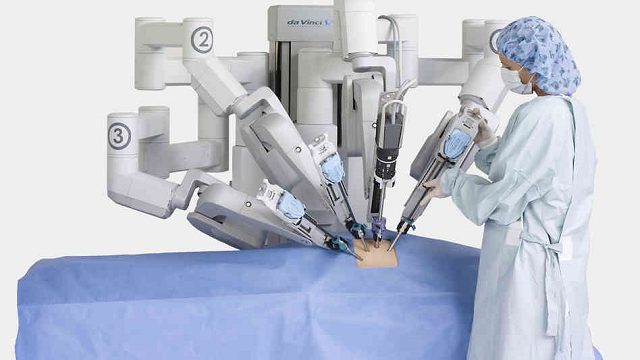
\includegraphics[width=1.1\pdfpagewidth]{da_vincy}%
%	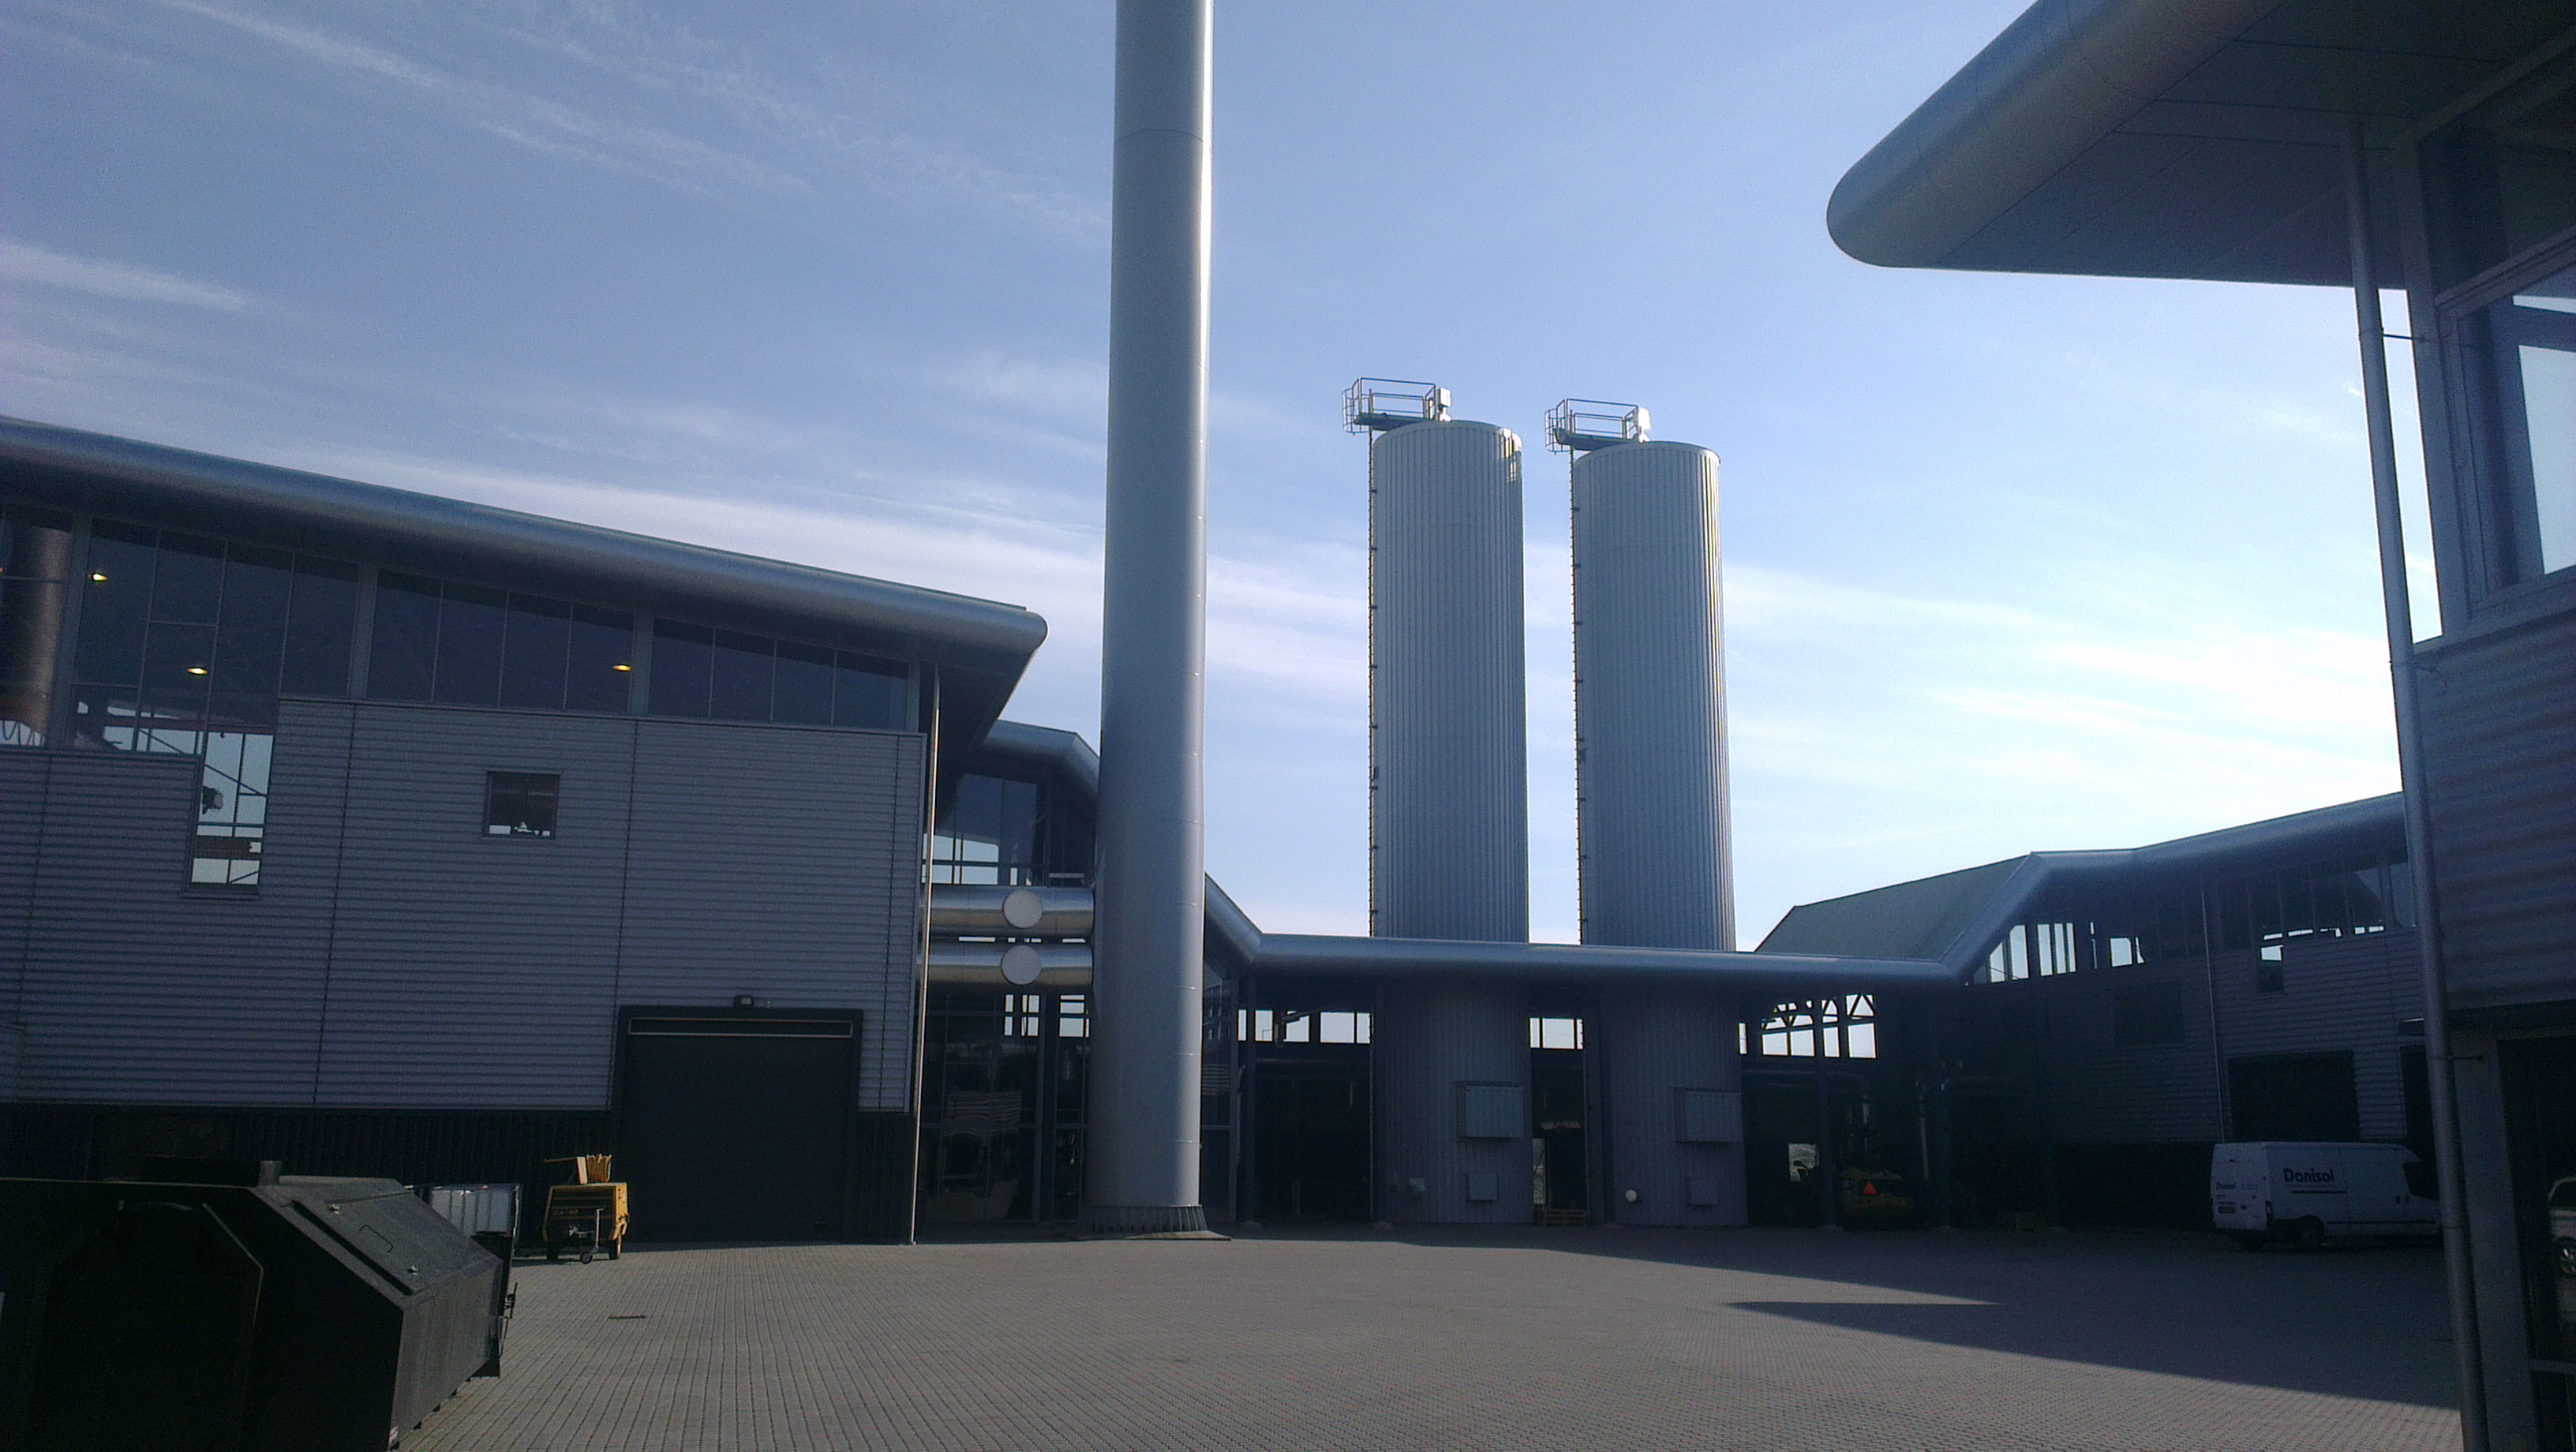
\includegraphics[width=0.45\pdfpagewidth]{formalia/2014-02-25 12.05.42.jpg}%	\caption{Virkningsgrad af den testede A/B hi-fi-forst�rker}
%\label{img_100wtest_linear}
\end{figure}
%\includepdf[scale=0.8,pages=1,pagecommand=\subsection{blub}]{testpdf}
%
\vspace{1cm}
\textsc{\Large \\
%Christian K�cks Lykkegaard \\
%s\\
%Economy track\\
%Elektronik \& IT\\
%Nordic Centre\\
%Fudan University\\
%September 27th 2012 \\
\textbf{School of Information and Communication Technology} \\
{\color{white}{..}}\\
Electronics \& IT\\
%s\\
Control and Automation \\
Final Thesis - CA4 Gr. 1032 \\
%Elektronik \& IT\\
Aalborg University\\
May 27$^\text{th}$ 2015\\
}\\
\end{titlepage}

\newpage
%\fchapter{}
\thispagestyle{empty}
%\begin{titlepage}
\vfil\null
\begin{center}
\bigskip \bigskip \bigskip
\vspace{1.0in}
\large
\bigskip \bigskip
\end{center} 
\normalsize
\vfil\null
\clearemptydoublepage
%\end{titlepage}

\thispagestyle{empty}
\begin{titlepage}


{\samepage 

\parbox{0.9\textwidth}{  
\raisebox{-15mm}{
\includegraphics[height=3.5cm]{AAU_LOGO_RGB_UK.png}}
\hfill{\footnotesize\noindent
\begin{tabular}{l}
            \textbf{School of Information and}\\
            \textbf{Communication Technology} \\
            Fredrik Bajers Vej 7 \\
            9220 Aalborg �st	\\
            Phone 99 40 86 00\\
            Fax 99 40 98 40\\
            http://www.es.aau.dk
\end{tabular}}}
\vspace{5mm}

    
\begin{tabular}{cc}
\parbox{7cm}{   
        {\bf Title:} Da Vinci Surgical Robot Automation \\        
        {\bf Master Thesis:} Control \& Automation\\              
        {\bf Project period:} Feb. $2^\text{nd} -$ June 3$^\text{rd}$ 2015\\
        {\bf Project group:} CA 15gr1032\\
        {\bf Participants:}\\
        \vspace{5mm}

\begin{minipage}[b]{0.7\linewidth}               	
     \underline{\phantom{JAERJAERJAERJAERoglidtmeretekst}}\\
      Britt Louise Jakobsen 
      
      \vspace{3mm}
	  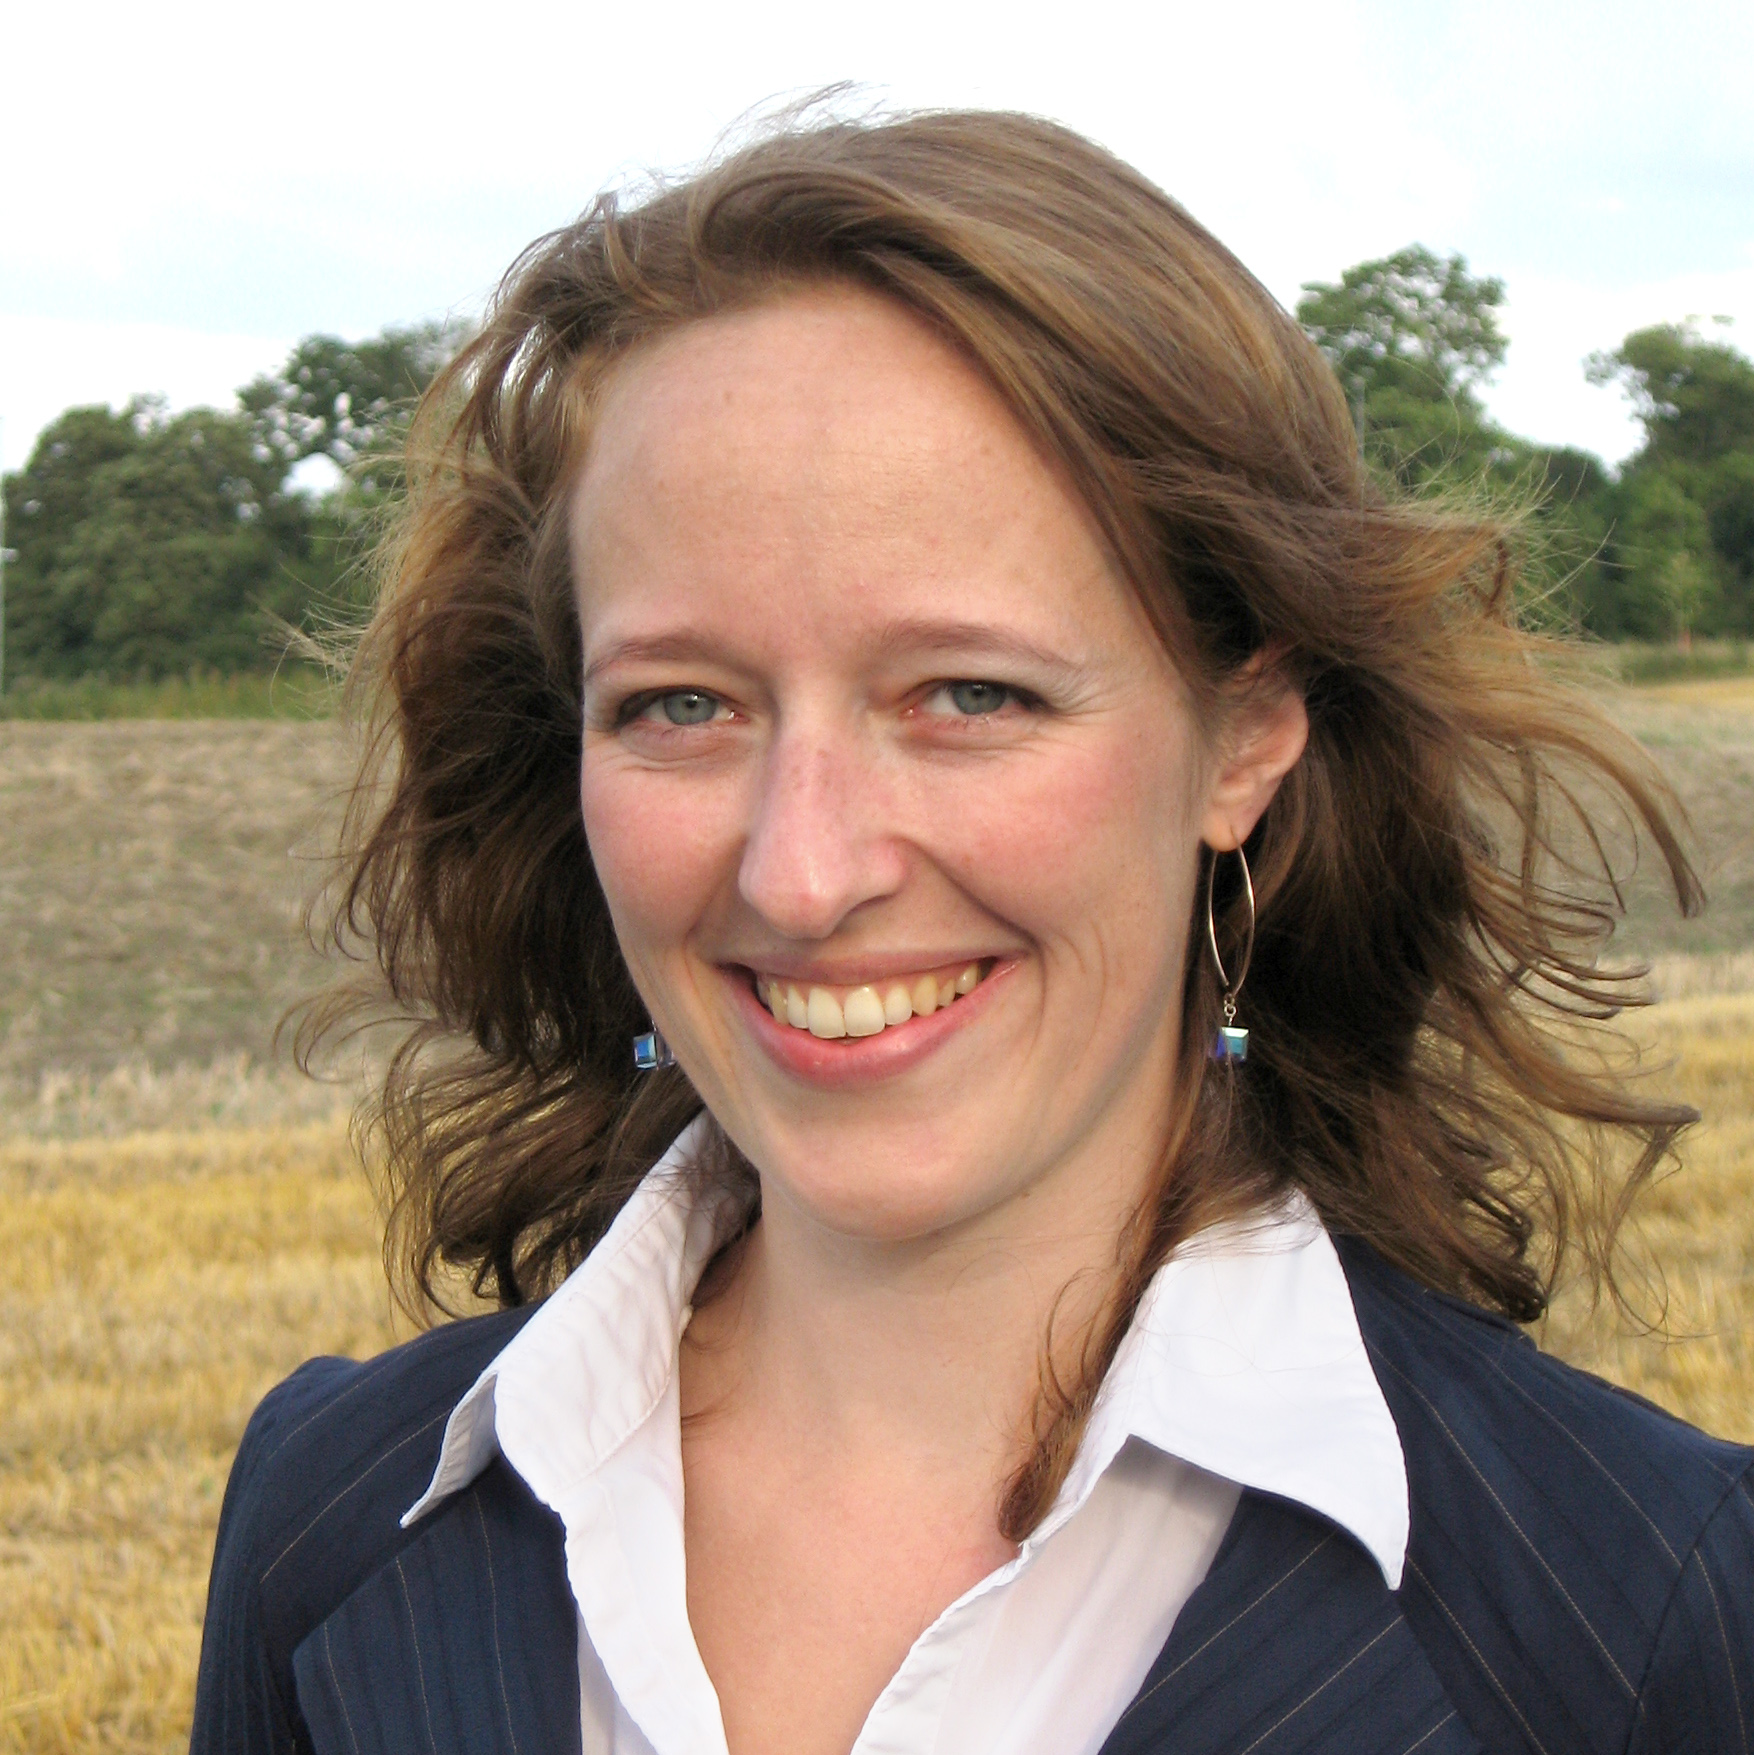
\includegraphics[width=0.52\textwidth]{IMG_3568_square.jpg}
\end{minipage}
  
\begin{minipage}[b]{0.7\linewidth}
   \vspace{10mm}
    \underline{\phantom{JAERJAERJAERJAERoglidtmeretekst}}\\
     Christian K{\o}cks Lykkegaard 

	\vspace{3mm}
	\includegraphics[width=0.52\textwidth]{IMG_3380.pdf}
\end{minipage}

\vspace{6mm}			
          
{\bf Supervisors:} \\
Prof. Rafa\l{} Wi\'{s}niewski\\
%Postdoc. Kasper Vinther\\
Ph.D. Tobias Leth\\
Assist. Prof. Christoffer Sloth\\
Postdoc. Karl Damkj�r Hansen\\  
               
        
{\bf Existing copies:} 5\\
{\bf Report:} \pageref{totalpage} pages \\
{\bf Appendix:} \pagedifference{appendixbegin}{appendixend} pages \\
\textbf{Attached:} 1 CD \\\\

\vfill } &
      
\parbox{7cm}{
\vspace{2mm}
\hfill 
\begin{tabular}{l}
      {\bf Abstract:}\bigskip \\
      \fbox{
      \parbox{7cm}{\bigskip
            {\vfill{\small In the course of the last few decades, robotic sur\-gery has become the  preferred type of operation within certain types of surgery, allowing the surgeon to perform precision procedures causing the patient a minimal amount of scarring while maintaining a exceptional overview of the operation site for the surgeon.


Advances are made within automation in the control of the robotic tools, providing the surgeon with more freedom and higher precision when performing operations. This thesis contributes to this advancement  through the use of barrier certificates with which safety of the automated control system can be guaranteed.


Control systems are developed for a number of use cases within robotic surgery for which safety  is certified through the construction of a barrier enclosing areas termed unsafe thus guaranteeing that the robotic tool will never cross this barrier. Two different approaches are taken: design of safety controllers based on manually constructed control barrier functions, and analytic verification of system safety using a software tool to construct the certificates.


The controllers are implemented on a first generation da Vinci surgical robot, and safety is verified for the developed control systems thus demonstrating the applicability of the theory of barrier certificates.


 \bigskip}}
      }\hspace{0.2em}}
\end{tabular}}

\end{tabular}

\vspace{-3mm}
\hspace{2mm}
\parbox{18cm}{
\noindent\footnotesize\textit{
\begin{flushleft} 
	The content of this report is freely available, but publication (with source reference) may only take place by agreement with the authors.	
\end{flushleft}}}
    
}
\end{titlepage}
\newpage
%\fchapter{}
\thispagestyle{empty}
%\begin{titlepage}
\vfil\null
\begin{center}
\bigskip \bigskip \bigskip
\vspace{1.0in}
\large
\bigskip \bigskip
\end{center} 
\normalsize
\vfil\null
\clearemptydoublepage
%\end{titlepage}

\setcounter{page}{1}
\renewcommand{\thepage}{\Roman{page}}

%\newgeometry{left=4.5cm,top=-0.5cm,bottom=2cm,textheight=28cm,includefoot,textwidth=16cm}
\chapter*{Preface}
\vspace*{-2mm}
This report documents the development process of a safe controller for automation of a surgical robot arm with patient safety guaranteed through barrier certificates. %, preventing the robot tool from entering predefined unsafe regions. 
The access to robot measurement data and opportunity to implement a controller heavily benefits from the previous work carried out on the da Vinci surgical robot in the Control Laboratory at Aalborg University.
The project is rated at 30 ECTS-points, and the work is conducted by the 4$^\text{th}$ semester group 1032 within the graduate program in Control and Automation at Aalborg University during the spring of 2015.


%The target group is supervisors, students and other interested parties at the School of Information and Communication Technology at the The Faculty of Engineering and Science.

\vspace*{-2mm}
\section*{Reading Guide}
\vspace*{-2mm}
The primary focus of this report is to design a controller and a barrier certificate, the certificate guaranteeing the safe control of a surgical robot, as an approach to draw closer to the possibility of implementing automated control tasks by surgical robots. 
%Controllers and certificates are designed for static as well as dynamic boundaries of unsafe regions, such as e.g. a beating heart.
After an introduction into surgical robotics and the definition of barrier certificates, two approaches to the design problem are described:
\vspace*{-3mm}
\begin{itemize}
\itemsep-1.4mm
\item Explicit approach: A barrier certificate is constructed and a safe controller is designed according to the method described in \citep{bib:org_control}.
\item Analytic approach: A controller is designed, criteria are constructed for a barrier certificate and  safety is verified by use of Putinar's Positivstellensatz.
%\item \autoref{part:closure} Discussion \textcolor{red}{REWRITE!!!}
\end{itemize}
\vspace*{-2mm}

Symbols, acronyms and a glossary are presented in the nomenclature before the main report.
A variant of the Harvard referencing is used for citations, with the author and publication year of the source given in square brackets, e.g. [Lasserre 78], and sources listed in the bibliography at the end of the main report. % contains all references used in the report. Books are indicated with author, title, publisher, year and ISBN. Web pages are indicated with author, title and year.
%Chapters in the main report are numerally numbered while appendices are alphabetically numbered.
A comprehensive appendix is included after the bibliography, containing introductions to the used software, detailed derivations, measurement logs and source code.
A digital copy of this report along with cited references, source code and simulation results can be found on the enclosed CD.

\vspace*{-2mm}
\section*{Acknowledgements}
\vspace*{-2mm}
The authors wish to thank Assistant Engineer Simon Jensen for a thorough introduction to the custom made AAU da Vinci hardware and design of a dynamic heart phantom platform; Ph.D. Tobias Leth for guidance in reference frame construction for robot kinematics;  Post Doc. Karl Damkj\ae r Hansen for an introduction to the AAU da Vinci robot operative system and help in implementing inverse kinematics; and Assistant Professor Christoffer Sloth for help and guidance with the theory behind barrier certificates and the use of SOSTOOLS.

Last but not least, it is desired to thank chief surgeon Johan Poulsen, robot assistant nurse Jane Petersson and surgeon Grazvydas Tuckus for sharing their insights in the use of surgical robotics and allowing the authors to attend a robotic surgery at Aalborg University Hospital.

%It is the wish of the authors to express a special appreciation to..

%\restoregeometry % efter denne side bruges de indstillinger der er sat i preamble
\newpage
%\fchapter{}
\thispagestyle{empty}
%\begin{titlepage}
\vfil\null
\begin{center}
\bigskip \bigskip \bigskip
\vspace{1.0in}
\large
\bigskip \bigskip
\end{center} 
\normalsize
\vfil\null
\clearemptydoublepage
%\end{titlepage}

\setlength\parskip{0ex}
\tableofcontents
\setlength\parskip{1ex}

\chapter*{Nomenclature}\label{chap:acronym}
\addcontentsline{toc}{chapter}{Nomenclature} % Adds chapter to TOC even though it is unnumbered
\printglossary[style=mcoltree,title=Glossary] %Print the glossary			%style=altlist
\printglossary[type=\acronymtype,style=glossary2col] %Print list of acronyms
\printglossary[type=symbols,style=altlong4col] %Print list of symbols
\clearpage

\section*{General Nomenclature Remarks}
\vspace{0.1cm}
\begin{itemize}
\item A dot above symbols indicate exclusively the time derivative, e.g. $\dot{x} = \dfrac{d}{dt}x(t)$
\item Well, maybe there is more
\item Or even more..
\end{itemize}

\textcolor{white}{\gls{analytic_func} \gls{rational_func} \gls{proper_func} \gls{injective_func} \gls{surjective_func} \gls{bijective_func} \gls{lipschitz} \gls{compact_space} \gls{hurwitz} \gls{dimension} \gls{extrinsic} \gls{intrinsic}}


\textcolor{red}{something simlar to this from \citep{bib:barrier_prajna}}
Notations: Most of the notations are standard. We denote
the set of real numbers by and the Euclidean n-space by $\mathbb{R}$.
The trace of an nxn matrix M, i.e., the sum of its diagonal elements,
is denoted by Tr(M). By f:X->Y we mean a function
mapping X subset Rn to Y subset Rm. We denote the spaces of
k-times continuously differentiable functions mapping
to Rm by Ck(X,Rm), and when m=1 we will write Ck(X).
Correspondingly, the spaces of continuous functions on are
denoted by C(X,Rn) and C(X). For a differentiable function
F:Rn->R, we use dF/dx(x) to denote the row vector
of partial derivatives of F with respect to x1,..xn. The Hessian
of a twice-differentiable function F:Rn->R is denoted
by d2F/dx2(x).

\cleardoublepage
\setcounter{page}{1}
\renewcommand{\thepage}{\arabic{page}}

\chapter{Introduction}\label{chap:intro}
In minimally invasive surgery (MIS), as opposed to traditional open surgery, only small incisions are made in the patient's abdomen or pelvis in order to gain access to the area under surgery, hence causing less trauma beyond this confined area. This in general provides the patient with quicker recovery, shorter hospital stay and less scarring.
One type of MIS is laparoscopy, invented in the beginning of the 20th century \citep{bib:laparoscopy}, where thin metal telescopes (laparoscopes) with specialized surgical tools attached are inserted into the patient through trocars, allowing the surgeon to maneuver the tools in the inflated abdomen guided by visual feedback from a flexible miniature camera (endoscope) inserted alongside the surgical tools \citep{bib:fascrs}.
In the 1980s robotic laparoscopic surgery was introduced as a master-slave system, where the surgeon controls a robot arm holding the surgical tools from a master console, instead of manipulating the instruments manually.

\section{Highlights in the Development of Surgical Robotics}
While the idea of roboticized telemedicine dates back to 1925 \citep{bib:telemed_predict}, the development of telesurgery was founded by NASA (National Aeronautics and Space Administration) in the 1970s \citep{bib:telesurg_history} combining research within virtual reality, robotics and medicine \citep{bib:brown_univ}, and the first robotic surgery procedure was accomplished in 1985 \citep{bib:telesurg_history}, followed by the first laparoscopic robotic surgical procedure in 1987 \citep{bib:brown_univ}.
The major research within telesurgery was funded by DARPA (Defence Advanced Research Project Administration, research administration under the U.S. Department of Defence) in the early 1990s, and two main teleoperation systems were developed from this research: da Vinci (from Intuitive Surgical) and Zeus (from Computer Motion) \citep{bib:telesurg_history}.

The first commercially available surgical robot ROBODOC (from Curexo) was introduced and performed the first robotic joint replacement surgery in 1992, and in 1994 the AESOP (from Computer Motion) was the first robotic system approved by the FDA (U.S. Food and Drug Administration) for general surgery \citep[p 74]{bib:telesurg_history,bib:surgical_book}.

In the early 1990s the U.S. Army developed MASH (Mobile Advanced Surgical Hospital) for loading and teleoperating wounded soldiers in vehicular operating rooms \citep{bib:brown_univ}, and in 1993 the idea for a robotic slave manipulator arm was conceived by Madhani after watching an episode of the tv-show M*A*S*H [SurgRob], and he created the Black Falcon during his work at MIT \citep{bib:black_falcon} later becoming he prototype of the da Vinci arms.

In 1996 the first tests were performed demonstrating the successful use of telementoring and telemanipulation of the endoscope by a surgeon placed several 100 m away from the operating room \citep{bib:telesurg_history}. 
In the late 1990s NASA and DARPA sponsored research within light-weight and deployable space surgical robotics for remote teleoperation, resulting in two main robotic systems: the Raven (from University of Washington) and M7 (from SRI International) [SurgRob].

In 1998 Zeus (from Computer Motion) was introduced and performed the first fully endoscopic robotic surgery and the initial beating-heart totally endoscopic coronary bypass procedure \citep{bib:brown_univ} and in 2000 da Vinci (from Intuitive Surgical) became the first robotic surgical system  to be approved by the FDA for general laparoscopic surgery \citep{bib:mddi}.

The first transatlantic telesurgical procedure, the Lindbergh Operation, was performed in 2001 by a team of French doctors in New York manipulating the arms of a Zeus robot to perform a gall bladder operation on a patient in Strasbourg \citep{bib:telesurg_history}. More research into remotely telementored and teleoperated robotic surgery was performed in the 2000s with the NEEMO (NASA Extreme Environment Mission Operations) projects in the Aquarius undersea lab in Florida, in 2003 with Zeus controlled from Ontario 2500 km away \citep[pp 75, 81]{bib:surgical_book} and in 2006 and 2007 with Raven and M7 controlled from Seattle \citep[pp 28, 82]{bib:surgical_book}. 

In 2005 DARPA launched the Trauma Pod program for developing an unmanned autonomous and semi-autonomous mobile military operation platform, funding research for e.g. SRI and for the Raven project. The goal of the first phase of the project was achieved in 2007 with the successful demonstration of a prototype trauma pod consisting of a da Vinci robot, a MASH stretcher and a custom nurse robot \citep[p 30]{bib:surgical_book}. The second phase aims at miniaturizing and integrating the systems \citep[p 31]{bib:surgical_book}, and in 2005 a demonstration was performed by roboticists, surgeons, aerospace engineers and networking experts in the desert placing the Raven patient manipulator and the controller console 100 m apart and relaying the communication link via a drone \citep{bib:docatadist}.

%In 2006 the first-ever demonstration of unmanned telesurgery with M7 [SurgRob]
%
%M7 performed the world's first automated ultrasound guided tumor biopsy in 2007 [SurgRob]
%
%2008 neuroArm was first used to remove a brain tumor [SurgRob]

NASA's first experiment in a zero gravity environment was performed with an acceleration compensated M7 in 2007 on a parabolic flight \citep[pp 29, 76, 85]{bib:surgical_book}, and in 2011 NASA sent the humanoid robot Robonaut 2 to ISS (International Space Station), and it has since been trained in telemedicine [SurgRob].







\section{State-of-the-Art in Surgical Robotics}
Most surgical robots used for telesurgery are master-slave systems which can be fully controlled by the surgeon \citep{bib:raven_debride}. The patient manipulator consists of 2-4 robotic arms, each having 6-7 degrees of freedom (DOF) \citep{bib:raven_debride} including the arm, wrist and the end-effector (the laparoscopic tool), one of the arms holding a stereo-vision endoscope. The end-effectors are positioned by high-precision motors and are able to reach spaces a human hand cannot \citep{bib:docatadist}.
Development is progressing within flexible end-effector tools \citep[p 74]{bib:surgical_book}, but even microrobots entering the body through natural orifices and controlled via electromagnetic fields or nanosensors and -actuators are being developed [SurgRob].

The 3D visual feedback from the endoscope is sent to the master console which can have eye-tracking for adaptive field of view and safety stop if the surgeon's gaze is not fixed at the operation site [SurgRob]. The control signals for the surgical instrument are generated with the controller joystick, which scales the surgeon's movements down to micro-movements \citep{bib:intuitive_monopoly} steerable through the (zoomed) 3D visual feedback. It also filters away tremor, and development is made within haptic feedback to the joystick \citep[p 89]{bib:surgical_book}, enhancing the surgeon's feel, enabling greater dexterity, accuracy and stability than a human hand.

In the first generations of surgical robotics the master and slave had to be in the same room (as is the case with da Vinci) \citep{bib:telesurg_history,bib:raven_debride,bib:surgical_book}. Experiments and development are made within minimizing and coping with delays for long-distance telesurgery and within miniaturization and robustness of the surgical robotic systems for use in harsh environments such as war and space, e.g. for da Vinci's potentially closest competitor, the open-source Raven.

Robotic surgical procedures are beginning to show superiority to conventional surgery for some procedures, but is still considerably more ecpensive \citep{bib:docatadist}. In some cases robotic procedures are faster than conventional surgeon procedures [SurgRob], but still in other it is much slower \citep{bib:raven_ii,bib:raven_debride}.
Autonomous procedures are still only implemented for entirely pre-planned motions of an operation, and depending on the type of operation not all subtasks in an operation are suited for autonomy \citep{bib:raven_debride,bib:raven_ii}.


\textcolor{red}{New generation: surgical care not only to soldiers but also to remote locations lacking specialized physicians. - better tactile feedback because the surgeon needs to feel the tissue and the difference in its stiffness}

Although the feasibility of conducting surgical interventions remotely has been demonstrated, there has not been market or clinical drivers strong enough to justify its implementation \citep[p 38]{bib:surgical_book}

\subsection{The da Vinci Surgical System}
Although several FDA approved robotic surgical systems exist, da Vinci is still the only commercially available system \citep{bib:docatadist,bib:intuitive_monopoly}. The first da Vinci prototype was developed at SRI under contract with the U.S. Army in the late 1980s [MDD], \citep{bib:brown_univ}, and in the early 1990s DARPA invested in the research \citep[p 74]{bib:surgical_book}. The the mid 1990s SRI licensed the manipulator design of Madhani along with many other patents, and in 1995 SRI founded Insuitive Surgical and the focus shifted from battlefield to commercial use in hospitals \citep{bib:intuitive_monopoly}.
In 1997 the first human trials were performed \citep{bib:intuitive_monopoly}, in 1999 the first market-ready da Vinci began tests [SurgRob] and the system was first approved by the FDA in 2000 \citep{bib:intuitive_monopoly,bib:brown_univ}. From 2000 until the merger in 2003 Intuitive Surgical and Computer Motion had a number of lengthy patent litigations \citep{bib:intuitive_monopoly,bib:telesurg_history}.

The da Vinci Surgical System still has the predominant market share with more than 3000 units installed worldwide due to being the first-mover in the field and due to their many patents \citep{bib:intuitive_monopoly}, and has only had one serious case of a patient dying after surgery (2002) [SurgRob].
The expiration of their patents in 2015 and 2016 \citep{bib:intuitive_monopoly} shows promise of many other robotic surgery systems entering the market, as both American, Canadian, European and not least Asian similar systems exist that are considerably cheaper than the da Vinci, and also more lightweight.

In 2013 Intuitive released the da Vinci Research Kit platform, built from mechanical components from first generation da Vinci (two arms and a surgeon console), open-source electronics and university-developed software \citep{bib:raven_observ}.

\subsection{The Raven Surgical Robot}
One potential challenger to da Vinci is the Raven \cite{bib:mddi}, an light-weight open-architecture 2-armed surgical robot \citep{bib:raven_debride,bib:raven_ii} originally developed by University of Washington funded by multiple U.S. government agencies including the Army and the Department of Defence (DoD) \citep[p 27]{bib:surgical_book}.
Raven-II is installed at 10 different universities in the U.S. and one in France \citep{bib:raven_ii}, sharing research innovations and using open-source software (including the ROS middleware) to create surgery subtasks \citep{bib:raven_debride}. 
As Intuitive Surgical's patents gradually expire the University of Washington is considering the possibility of spinning off the Raven into a start-up company \citep{bib:economist}.

The Raven robot is focused on remote telesurgery (with notable latency) in harsh conditions \citep{bib:docatadist}, and research at University of California has been made in teaching a computer model to autonomously mimic laparoscopic surgeons from recordings dynamic and kinematic data of their motions in a multi-state statistical Hidden Markov Model \citep{bib:economist}. 
The primary difficulty reported from controlling the Raven has been state estimation, necessary because of the uncertainty inherent in actuators and encoders connected to flexible elements via long cables \citep{bib:raven_debride} and the necessity of collision avoidance of the arms.



































\section{Focus of this Project}
Our focus:
safety
make forbidden areas where the robot cannot enter

ROS middleware layer as in Raven.
Prior work: designing planning and control algorithms for autonomous execution of several surgical subtasks (knot tying, suturing), advances in motion planning, control and perception: integrated task and motion planning ofhigh level task planning using state machines, and motion planning for low level planning algorithm  \citep{bib:raven_debride}
Raven-II inverse control process (not primarily to estimate the pose, in which case standard estimation methods like Kalman would be appropriate) is to calculate, give an desired true pose, the input pose to send the control sw to reach the desired true pose (detected pose with vision system assumed to be the true pose), estimate between measurements using updates from forward kinematics \citep{bib:raven_debride}.
da Vinci Research Kit: learning from demonstrations/by observation. Targets considered form convex regions spherical/linear. Patient Side Manipulators manipulates the instruments about a fixed point called the remote center of motion \citep{bib:raven_observ}.
DLR MIRo integrates torque sensing capabilities on the joint level, cosisting of actuation- position sensing- and torque sensing modules, can run in torque and impedance control mode. Virtual springs/potential fields are used to impose constraint forces preventing the robot from  entering predefined areas.


One should certainly take the risk of patient trauma when an automated surgery is conducted into account. This is seen in Therac-25. It is therefore a necessity to formally prove that the procedure is safe as seen in \citep{bib:safety}
\section{Technical Overview}
A simplified overview of the overall setup is provided in \autoref{fig:overview} as a block diagram. The setup is physically located at the department of Control and Automation at Aalborg University in the laboratory. The figure is structured with the highest abstraction layer at the top (i.e. the ROS (Robotic Operation System) - a software framework for robots [ROS artikkel]) environment which establish a wireless TCP/IP communication channel receiving all positions from the robot as feedback. It produces likewise positioning control signals to the NI (National Instruments) single board RIOs (Reconfigurable Input/Output) which handle all input/output communication with the user. The NI single board RIOs consist of a primary and a secondary board. The reason for having two RIO boards is solely the lack of input/outputs on one board.

The RIO boards direct the control signals to a cascaded controller taking in a velocity reference from the user and delivers a current control signal to the ESCON motor driver. The velocity and current controller are implemented in FPGA based hardware to ensure sufficient controller speed relative to the system \citep{bib:robot_paper}. The ESCON motor driver manage advanced processing and delivers essentially an appropriate PWM signal for the  actuators in form of seven maxon motors which represent the lowest abstraction layer located at the bottom of the figure.

The NI single board RIOs handle concurrently most safety precautions and enabling/disabling of the arm itself (see appendix ?? for location of the arm) through solenoids.
\begin{figure}[H]
	\center
	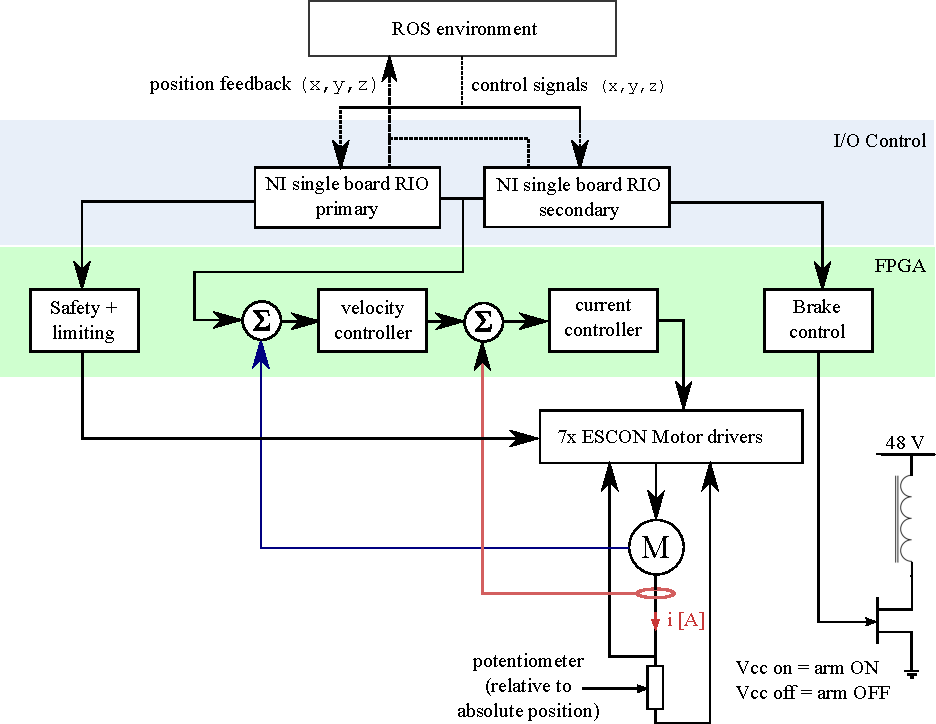
\includegraphics[width=0.95\textwidth]{overview.pdf}	\caption{This is a nice figure. Here illustrated for hand roll master.}
	\label{fig:overview}
\end{figure}
The focus of this thesis is the highest abstraction layer, i.e.the ROS environment. The purpose here primary constitute implementation of:
\begin{itemize}
\item Everything that require heavy processing \citep{bib:robot_paper}.
\item Non real-time processing or tasks with loose timing constraints \citep{bib:robot_paper}.
\end{itemize}
The above pool of stipulations will essentially and practically entail the follow main topics of this thesis:
\begin{itemize}
\item All user interaction
\item Positioning control loop
\item Path planning
\end{itemize}

\chapter{Safety Guarantee by Barrier Certificates}\label{chap:barrier_cerificates}
	A crucial matter when designing a controller for automated operation of robotic surgery tools is the necessity of guaranteed patient safety. The system has to not only be able to prevent the surgery tool from entering certain regions, e.g. penetrating the wall of the heart or cutting an artery, but to guarantee that this cannot happen under any circumstances.


Casting the controller design problem as an optimization problem with constraints, such as \gls{mpc}, could in principle guarantee that the tool would not enter a predefined area. Indeed, \gls{mpc} is a method which is very popular at the higher abstraction layers, such as setpoint control \citep{bib:mpc_simon} which is the case in this specific study. However, most solvers such as the Matlab plugin \texttt{cvx} requires convexity in the performance function and its constraints to be able to find a global minimum. This will at best be a lucky special case that unsafe regions can be defined through a convex function.  
Furthermore, \gls{mpc} is mostly used in systems with slow dynamics, i.e. dynamics where the time constant is measured in seconds or even minutes \citep{bib:mpc_slow}. This is obviously due to heavy online computations and numerous iterations. Systems containing these time constants are usually thermal systems and not mechanical systems. Additionally, the feasibility of the optimization problem is not very transparent and it is well known that \texttt{cvx} is very likely to crash due to infeasibility.
%, but a hard constraint would fail to follow the dynamics of a moving area boundary such as a beating heart. 

Another very elegant and computationally efficient approach to the safe controller analysis and design problem is the use of barrier certificates, which provide a formal proof of safe operation in infinite time horizon \citep{bib:prajna_framework,bib:safety}. This chapter describes the requirements for the construction of barrier certificates along with notation used in relation to these.
%


%dealing with those topics within robotic surgeries feature necessary conditions to guarantee the patient safety and to avert patient trauma .



\section{Constraints for a Barrier Certificate}\label{sec:safety-def}

When a barrier certificate can be found for a (closed-loop) dynamical system, the controller is guaranteed to be safe. In the following the notion of safety is defined in order to describe the guarantee extent of a barrier certificate. A general state-space representation of an $n$-dimensional non-linear system is considered:
\begin{equation}
\dot{\mathbf{x}} = f_{cl}(\mathbf{x}) + h(\mathbf{x})\,\mathbf{d} = f(\mathbf{x}) + g(\mathbf{x})\,\mathbf{u} + h(\mathbf{x})\,\mathbf{d}
\label{eq:general_statespace}
\end{equation}
\begin{tabular}{rl} 
where &  \\
\gls{x} &  is the state, $\mathbf{x}(t) \in \mathbb{R}^n$\\
\gls{u} & is the control input, $\mathbf{u}(t) \in \mathbb{R}^m$\\
\gls{d} & is the disturbance input, $\mathbf{d}(t) \in D \subseteq \mathbb{R}^p$ \\
\gls{f} & is a non-linear function, $f:\mathbb{R}^n \rightarrow \mathbb{R}^n$\\
\gls{g} & is a non-linear function, $g:\mathbb{R}^n \rightarrow \mathbb{R}^{n \times m}$\\
\gls{h} & is a non-linear function, $h:\mathbb{R}^n \rightarrow \mathbb{R}^{n \times p}$
\end{tabular}\\

Consider a subspace of the state-space $\mathcal{X}\subseteq\mathbb{R}^n$ defining e.g. the physically feasible states for the system in \autoref{eq:general_statespace}. Within this region $\mathcal{X}$, define the two non-intersecting subspaces $\mathcal{X}_u\subset\mathcal{X}$ and $\mathcal{X}_0\subseteq\mathcal{X}$, defining an unsafe  and a safe region, respectively. The unsafe region contains the states which the trajectory of the system must never enter, e.g. for a surgical robot this space could be the collection of veins and organs near the operation site, for which perforation is prohibited. The safe region contains all the states which the trajectory of the system is allowed to and may be required to enter, e.g. the operation site and a region for entering the area in the abdomen.
Now safety of a closed-loop control system is given according to \citep{bib:safety,bib:prajna_framework} as:
%\begin{exa}

\begin{defn}[Safety of a System]\label{def:safety}
Denote a trajectory starting in $x(0)=x_0$ and with bounded disturbance function $\bar{d}:\mathbb{R}_{\geq 0}\rightarrow D$ by $\phi_{x_0}^{\bar{d}}$, defined by 
\begin{equation}
\frac{d \phi_{x_0}^{\bar{d}} }{dt} = f_{cl}\left( \phi_{x_0}^{\bar{d}} (t) \right) + h\left( \phi_{x_0}^{\bar{d}} (t) \right) \bar{d}(t)
\end{equation}
The system $\Gamma_{cl} = (f_{cl},h,\mathcal{X},\mathcal{X}_0,\mathcal{X}_u,D)$ is unsafe if there exists a $t \in [0,$\gls{T}$]$ such that the trajectory $\phi_{\mathcal{X}_0}^{\bar{d}}:\,[0,T]\rightarrow \mathbb{R}^n$ with initial state $x_0\in \mathcal{X}_0$ and bounded disturbance function $\bar{d}$ satisfies
\begin{flalign}
\left( \phi_{\mathcal{X}_0}^{\bar{d}}([0,t]) \cap \mathcal{X}_u \right) \neq \emptyset \kk \text{and} \kk 
\phi_{\mathcal{X}_0}^{\bar{d}}([0,t]) \subseteq \mathcal{X}
\label{eq:defsafety}
\end{flalign}
\noindent
The system $\Gamma_{cl}$ is safe if there are no unsafe trajectories.
\end{defn}

%\vspace{-0.2cm}
%
%\begin{longtable}{p{.9\textwidth} p{.1\textwidth} p{.1\textwidth}} 
%Where  & & \\
%\gls{fcl} is a potential non-linear function with the closed loop characteristic:\\ \kk $f_\text{cl}: x \mapsto f(x)+g(x)k(x)$ where \gls{k} is the feedback gain with the map $k: \mathbb{R}^n \rightarrow \mathbb{R}^m$ & [$\cdot$] &  \\
%\gls{X} is the set of all allowed states & [$\cdot$] &  \\
%\gls{X0} is the set of all allowed initial states & [$\cdot$] &  \\
%\gls{Xu} is the set of all unsafe states & [$\cdot$] &  \\
%\gls{phi} is the set of all allowed initial conditions with the bounded disturbance input \gls{dbar} & [$\cdot$]
%\end{longtable}

A graphical interpretation of \autoref{eq:defsafety} is shown in \autoref{fig:defsafety}.

\begin{figure}[H]
	\center
	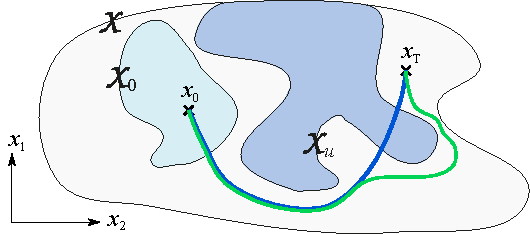
\includegraphics[width=0.6\textwidth]{safety.pdf}	
	\caption{Graphical interpretation of \autoref{eq:defsafety} in the state space. The blue trajectory is unsafe because $\left( \phi_{\mathcal{X}_0}^{\bar{d}}([0,t]) \cap \mathcal{X}_u \right) \neq \emptyset$, while the green trajectory is safe.}
	\label{fig:defsafety}
\end{figure}
%\end{exa}

Disturbances are not considered in the scope of this project, and hence $\mathbf{d}\in D$ is considered to be zero in the remainder of this thesis.

For the system in \autoref{eq:general_statespace} safety can be guaranteed if a barrier certificate for the system exists. A barrier certificate is defined as a function of the system state, satisfying a set of inequalities, entailing that its zero level set in the state space forms a barrier between the safe set of initial states $\mathcal{X}_0$ and the unsafe set $\mathcal{X}_u$, thereby certifying system safety \citep{bib:prajna_framework}.


If a barrier certificate can be defined, safety can be guaranteed for the closed-loop system in the region $\mathcal{X}$, with unsafe region $\mathcal{X}_u$, defined by positive values of the barrier function, and (safe) initial region $\mathcal{X}_0$, defined by non-positive values of the barrier function. In the below the notation $L_{f_{cl}}B(\mathbf{x})$ denotes the Lie derivative of \gls{bar} along the vector field of the closed-loop system $f_{cl}(\mathbf{x})$, corresponding to the time derivative of the barrier function i.e.
\begin{equation}
L_{f_{cl}}B(\mathbf{x})=\frac{dB(\mathbf{x})}{d\mathbf{x}}f_{cl}(\mathbf{x})=\frac{dB(\mathbf{x})}{d\mathbf{x}}\frac{d\mathbf{x}(t)}{dt}=\frac{dB(\mathbf{x}(t))}{dt}
\end{equation}

Requiring that the time derivative of the barrier function must be nonpositive on the entire set $\mathcal{X}$ (see \autoref{def:barrier_certificate}) corresponds to the value of the barrier function decreasing over time, hence seeking the minimum of the (convex) barrier certificate. Requiring the trajectory of the state to start within the safe set $\mathcal{X}_0$ this means that the trajectory will never cross the zero level set and enter the unsafe set $\mathcal{X}_u$, as this set only contains values of the barrier function larger than the initial value.

\begin{defn}[Barrier Certificate]\label{def:barrier_certificate}	
If a barrier certificate can be constructed as a continuous and differentiable function $B(\mathbf{x}):\mathcal{X} \rightarrow \mathbb{R}$ adhering to the following inequalities  \citep{bib:prajna_framework}:
\begin{subequations}\label{eq:barrier_constraints}
\begin{flalign}
B(\mathbf{x}) &\leq 0 \kk  \forall \hspace{2mm} \mathbf{x} \in \mathcal{X}_0  \label{cer1}\\
B(\mathbf{x}) &> 0  \kk  \forall \hspace{2mm} \mathbf{x} \in \mathcal{X}_u \label{cer2} \\
L_{f_{cl}}B(\mathbf{x}) &\leq 0 \kk  \forall \hspace{2mm} \mathbf{x} \in \mathcal{X} \label{cer3}
\end{flalign}
\end{subequations}
Then safety of the closed-loop system $f_{cl}(\mathbf{x})$, as defined in \autoref{def:safety}, is guaranteed. 
\end{defn}


From \autoref{eq:barrier_constraints} it can be seen that the function $B(\mathbf{x})$ must be constructed such that its zero level set delimits and separates the safe and the unsafe regions, while the Lie derivative constraint imposes that the derivative $dB(\mathbf{x})/d\mathbf{x}$ must have the opposite sign of the state derivative $d\mathbf{x}/dt$ for any state within the region $\mathcal{X}$, where $B(\mathbf{x})$ is defined. 
Note how according to \autoref{cer3} the barrier certificate requires mere stability and not asymptotic stability ($L_{f_{cl}}B(\mathbf{x})<0$) of the system trajectory. This is rarely enough when dealing with physical systems, however, mathematically it is sufficient.

Furthermore from \autoref{cer3} it is deduced that a controller incorporating the barrier certificate in its design will ensure stability if $B(\mathbf{x})$ has a finite minimum value. This entails that $B(\mathbf{x}) $ is radially unbounded if $\mathcal{X}$ encompasses the entire state-space:
\begin{equation}
\underset{\mathbf{x}\rightarrow \pm\infty}{\lim} B(\mathbf{x})= \infty \kk \text{if} \kk \mathcal{X}=\mathbb{R}^n
\end{equation}

\subsubsection{Nexus to Lyapunov Functions}
\vspace*{-3mm}
As it can be seen from \autoref{eq:barrier_constraints} the definition of a barrier certificate strongly resembles that of a Lyapunov function, and indeed the Lie derivative nonpositivity constraint is identical to the time derivative constraint to a Lyapunov function $V(\mathbf{x})$, a Lyapunov candidate function for a stable system given by
\vspace*{-5mm}
%\begin{equation}
%\dot{x}  = f(x) = \frac{d x}{d t} \qquad
%\left\{ \begin{array}{r l l}
%L_fB(x) \hspace*{-2mm}&= \tfrac{d B(x)}{d x} f(x) \hspace*{-2mm}&= \tfrac{d B(x)}{d x} \frac{d x}{d t}\\
%\dot{V}(x) \hspace*{-2mm}&= \tfrac{d V(x)}{d t} \hspace*{-2mm}&= \tfrac{d V(x)}{d x}\tfrac{d x}{d t}
%\end{array} \right. \label{eq:dBdt_dVdt}
%\end{equation}
\begin{subequations}\label{eq:lyap}
\begin{align}
V(\mathbf{x}) &> 0 \kk \forall \hspace{2mm}\mathbf{x} \in \mathbb{R}\setminus\{0\}\\
\dot{V}(\mathbf{x}) &\leq 0 \kk \forall \hspace{2mm}\mathbf{x} \in \mathbb{R} \label{eq:lyap_stable}
\end{align}	
and for a system with an asymptotically stable equilibrium in $\mathbf{x}=0$, \autoref{eq:lyap_stable} is replaced by
\vspace*{-2mm}
\begin{equation}
\dot{V}(\mathbf{x}) < 0 \kk \forall \hspace{2mm}\mathbf{x} \in \mathbb{R}\setminus\{0\}\label{eq:lyap_vdot_minus_criticalpoint}
\end{equation}
\end{subequations}
As such a barrier certificate can be seen as an offset Lyapunov function with negative values in the safe region. The stable focus may also be offset from $\mathbf{x}=0$. However, a barrier function may also take other (non-convex) forms. 



\section{Approaches to the Problem of Guaranteeing System Safety}
Two approaches to the problem of guaranteeing safety of a system through the construction of barrier certificates are used in the following: design of safe controllers and safety verification of control systems.

In \autoref{chap:cbf} a method of designing guaranteed safe controllers from barrier certificates is described, based on \citep{bib:org_control}. This method is used in chapters \ref{chap:cbf_1d_static} through \ref{chap:cbf_3d_static}, where barrier certificates are constructed by hand, and guaranteed safe controllers are designed and implemented on the da Vinci surgical robot. The safe controller is used in combination with a linear state space controller designed through pole placement for setpoint control in the safe region. In \autoref{chap:cbf_1d_static} and \ref{chap:cbf_1d_dynamic} system models of different orders are considered in 1D Cartesian space, with static and dynamic boundaries (zero level sets) of the barrier function, respectively, while in \autoref{chap:cbf_3d_static} a system model is considered in 3D Cartesian space. 

In \autoref{chap:putinar} a recasting of \autoref{def:barrier_certificate}  according to \citep{bib:sos_putinar_lasserre} is presented, allowing for automated construction of barrier certificates with an existing software toolbox for MATLAB. 
When a barrier certificate can be found using this toolbox, system safety is hereby certified.
In \autoref{chap:sostools} this method of safety verification is applied to linear position-control systems corresponding to the linear state space controllers presented in \autoref{chap:cbf_1d_static}.
%Similarly to \autoref{part:cbf} the following chapters verify controller safety for system models of different orders in 1D and 3D space, with static and dynamic boundaries (zero level sets) of the barrier function.
%\autoref{chap:sos_1d_static} \autoref{chap:sos_1d_dynamic} \autoref{chap:sos_3d_static} \autoref{chap:sos_3d_dynamic}



%The design of a safe controller features the property that a supplied control signal ensures compliance of the definition described in \autoref{sec:safety-def}.








\chapter{Controller Design from Control Barrier Functions}\label{chap:cbf}
	\glsreset{clf}\glsreset{cbf}
Based on \citep{bib:artstein}, which founded \gls{clf}s, a \gls{cbf} can be created \citep{bib:org_control}. With a system $\dot{x}=f(x)+g(x)u$, a \gls{cbf} exist if the below constraints are fulfilled:
\begin{flalign}
& x\in \mathcal{X}_u \hspace{0.3cm} \Rightarrow \hspace{0.3cm} B(x) > 0  \label{req1} \\
& L_gB(x) = 0 \hspace{0.3cm} \Rightarrow \hspace{0.3cm} L_fB(x) < 0 \label{req2} \\
& \{ x \in \mathcal{X} | B(x) \leq 0 \} \neq \emptyset \label{req3}
\end{flalign}
\vspace{-0.8cm}
\begin{longtable}{p{.9\textwidth} p{.1\textwidth} p{.1\textwidth}} 
Where  & & \\
$L_f(x)$ is the Lie derivative of $B(x)$ along the vector field  $f(x)$, i.e. $\frac{\partial B(x)}{\partial x}f(x)$ & [$\cdot$] \\ 
$L_f(x)$ is the Lie derivative of $B(x)$ along the vector field  $g(x)$, i.e. $\frac{\partial B(x)}{\partial x}g(x)$ & [$\cdot$] 
\end{longtable}
\vspace*{-0.2cm}
Taking a look at \autoref{req1} it states essentially the same as \autoref{cer2}, i.e. the unsafe area exist whenever $B(x)>0$. This makes it possible to design an unsafe region. \Autoref{req2} put forth the requirement that the gradient along the vector field $f(x)$ must point away from the barrier extremities whenever the input is with no significance (except for the critical point). \Autoref{req3} simply states that the safe area must contain some states as control otherwise is impossible.
\section{Safe Controller for Instrument Slide}
The slide movement is visualized in \autoref{fig:slidefig} and an overview of terms used in this section is found in \autoref{fig:safe:overview}.
\begin{figure}[H]
    \centering
    \begin{minipage}{.5\textwidth}
        \centering
        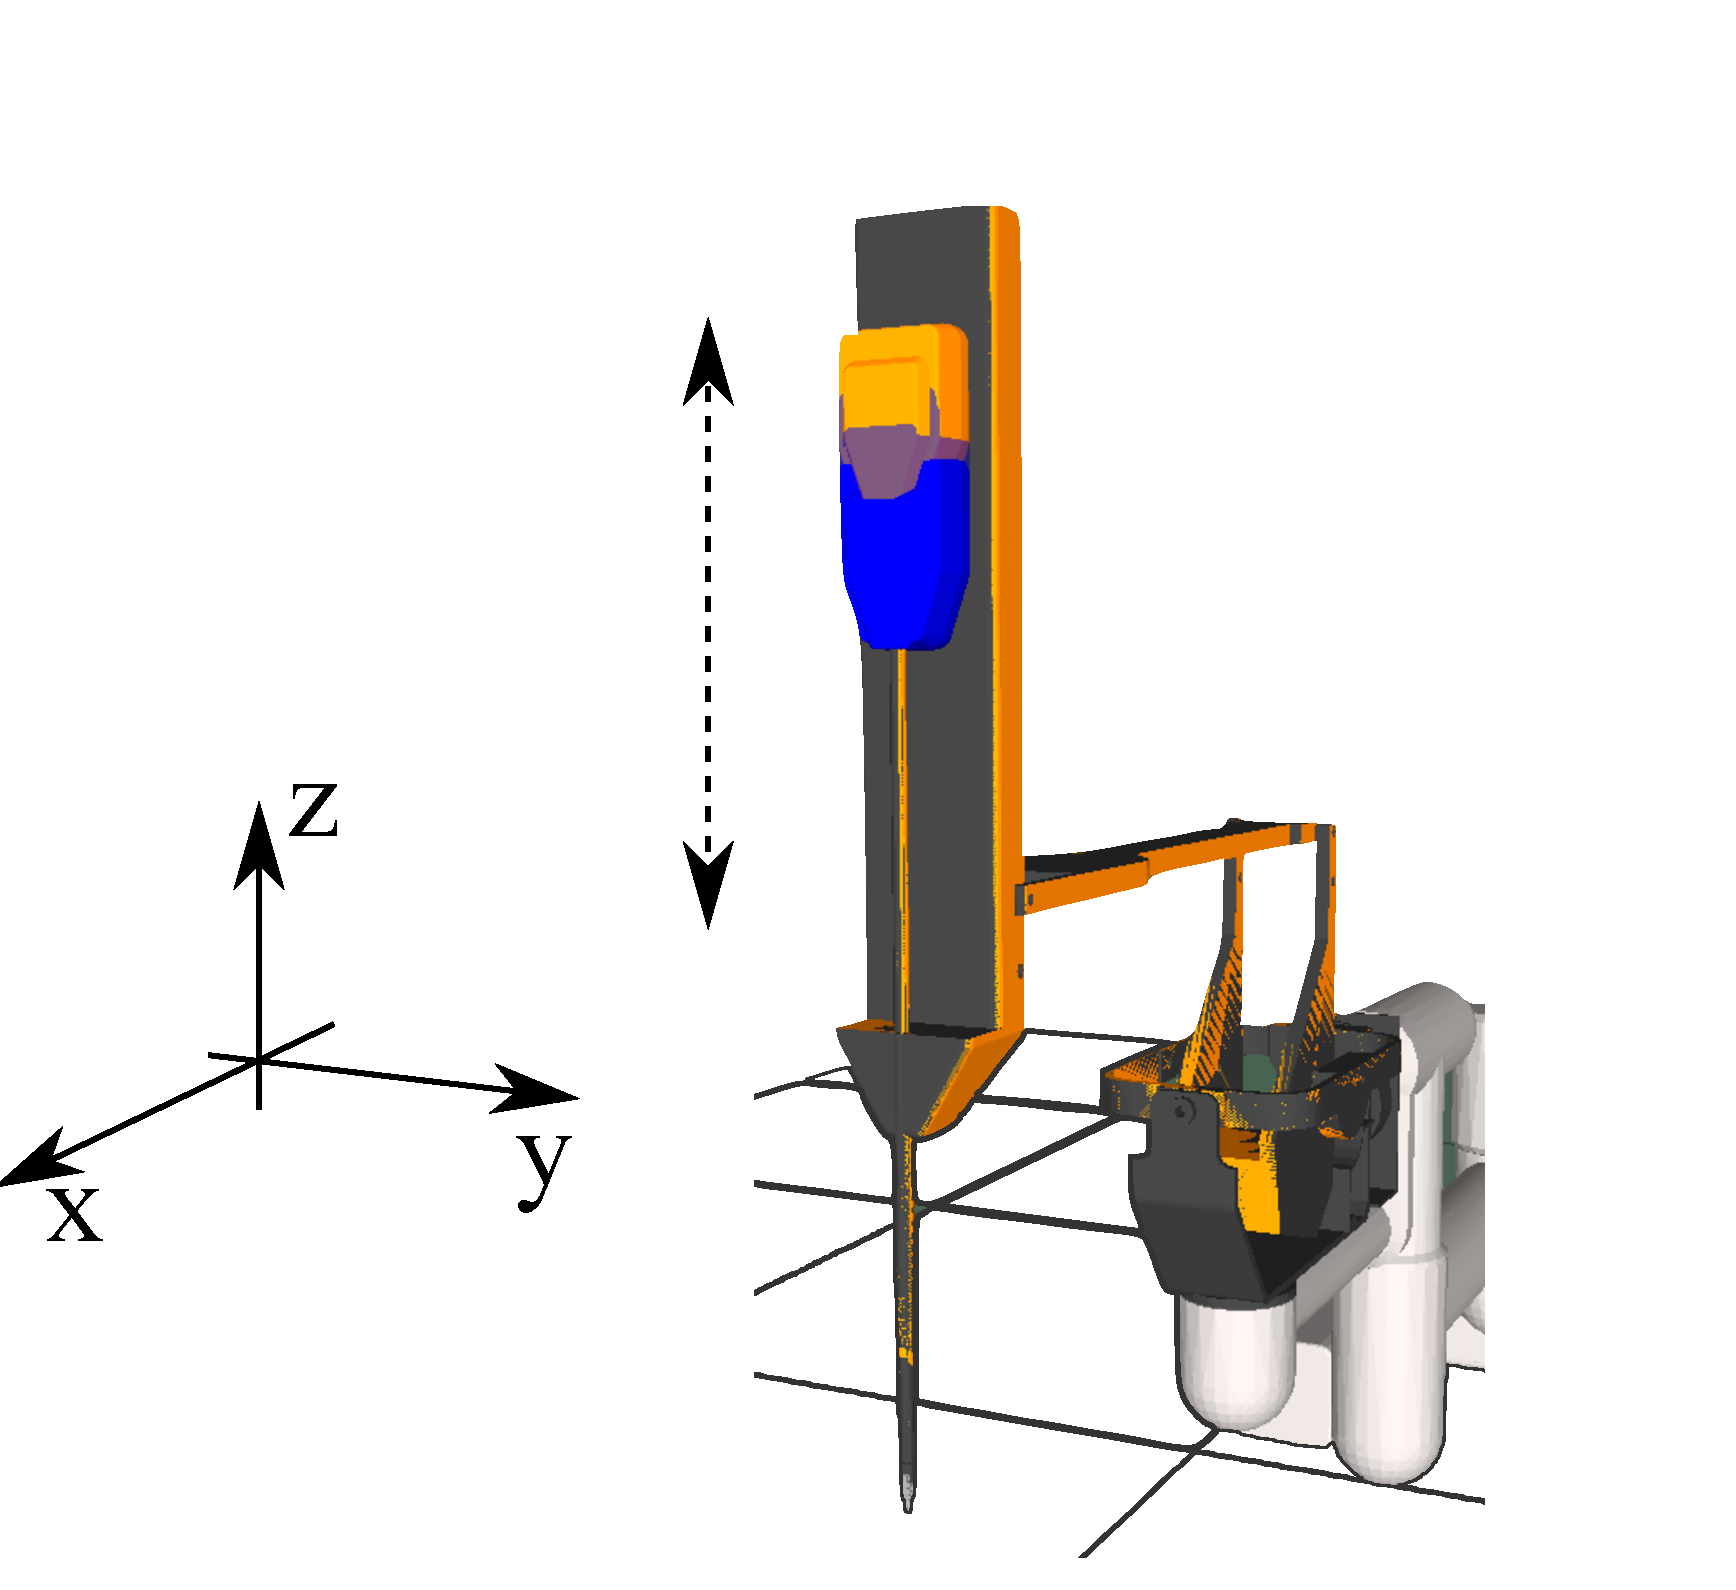
\includegraphics[width=0.73\linewidth]{slidemovefigure.pdf}
        \caption{Illustration of slide movement.}
        \label{fig:slidefig}
    \end{minipage}%
    \begin{minipage}{0.5\textwidth}
        \centering
        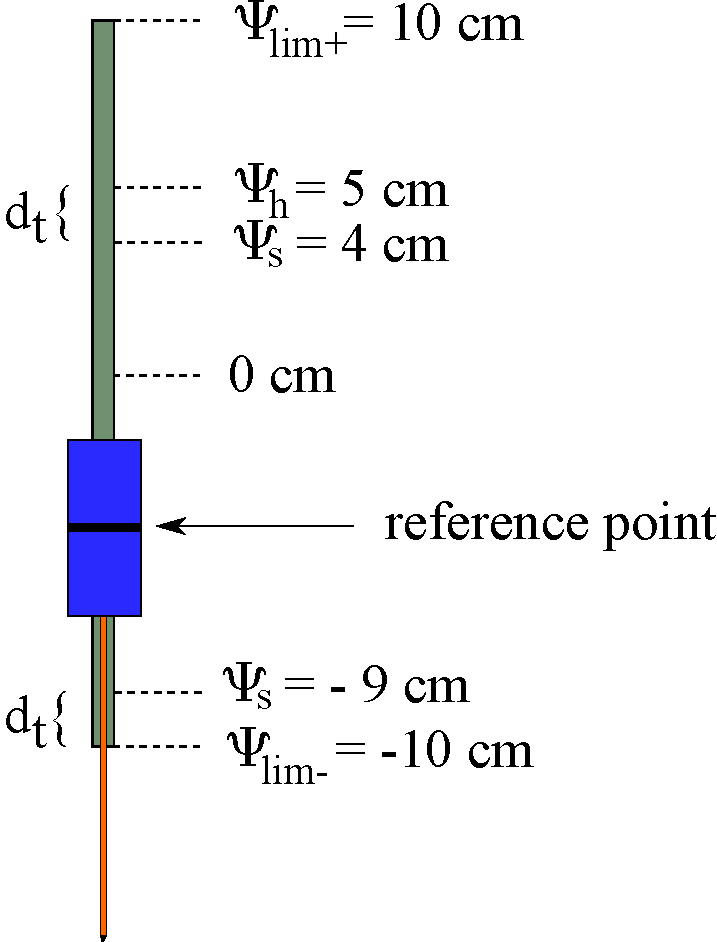
\includegraphics[width=0.7\linewidth]{slide_overview.pdf}
        \caption{Boundaries used in this section.}
        \label{fig:safe:overview}
    \end{minipage}
\end{figure}
A system model is required before any controller design may be initiated.
%\hspace{1cm }\texttt{rostopic echo joint\_states/position[6]} \hspace{0.2cm} {\color{blue}{\# Be sure to have the ROS environment correctly configured according to \autoref{app:ros}}}
\section{Modelling of Slide Movement}
 To obtain a model, a step response will be performed on the slide movement. The slide position can be measured by subscribing to the \texttt{joint\_state} topic in \gls{ros}. The experiment is described in further details in \autoref{app:meas}. To model the system, a step is added to the system. The step response is plotted in \autoref{fig:stepresponseslide}.
\begin{figure}[H]
\center
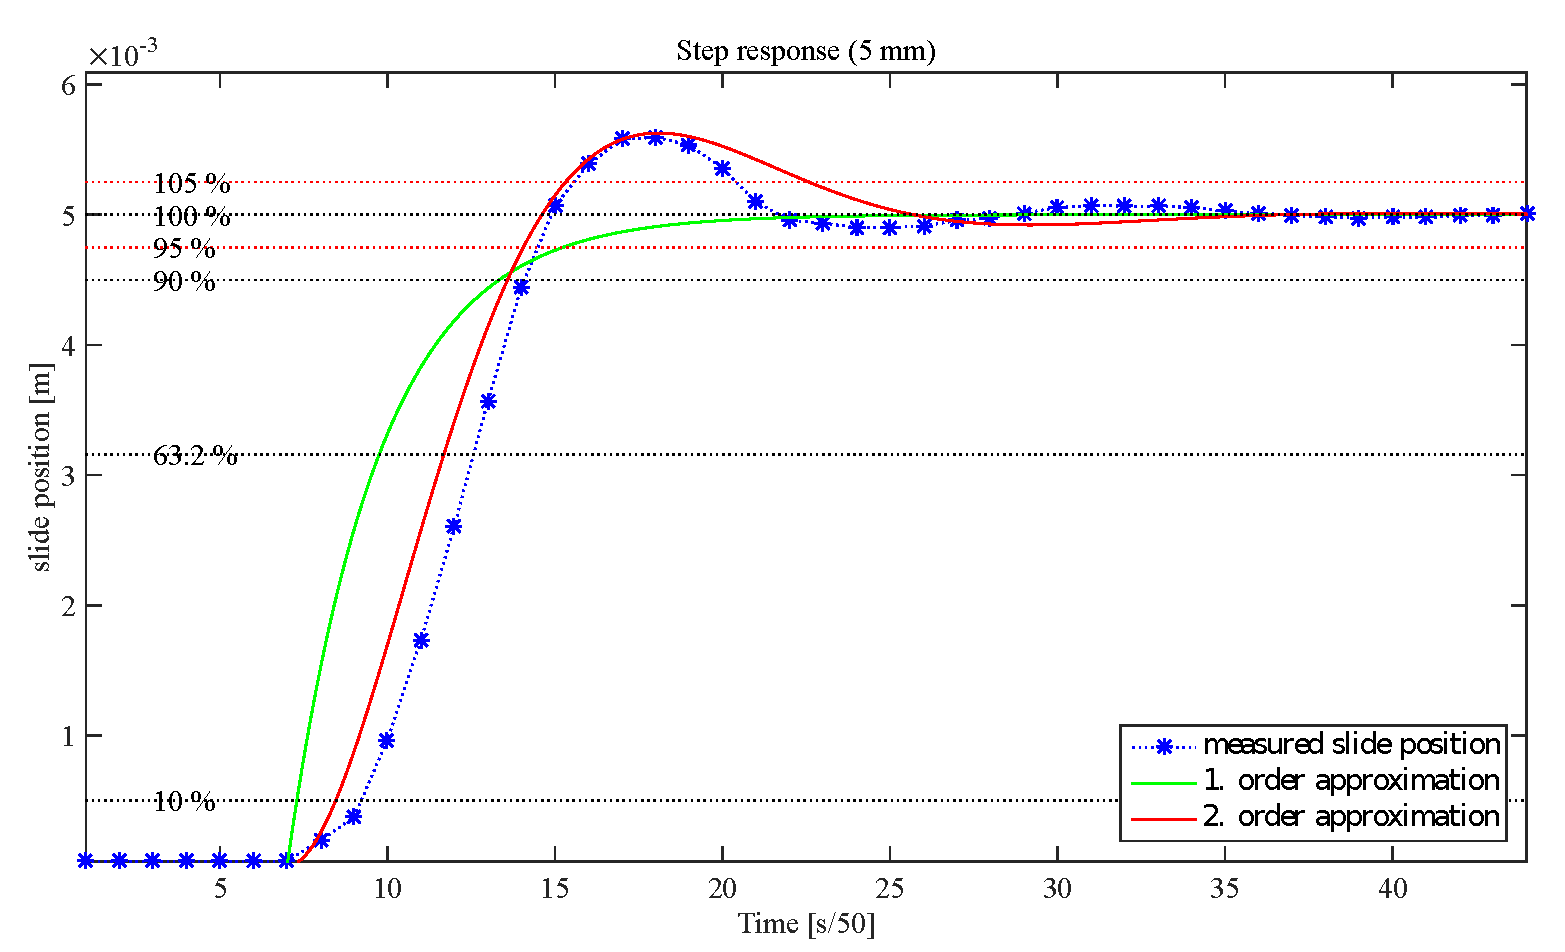
\includegraphics[scale=0.5]{step_slide.pdf}
\caption{Step response from 0\,mm to 5\,mm. Plot details and measurements can be found in \autoref{app:cd} as \texttt{matlab\_scripts/slide\_step/plot\_slide\_pos.m}}
\label{fig:stepresponseslide}
\end{figure}
It is clear that this could be well approximated with an underdamped second order model (complex roots), however for initial simplicity and because modelling is not a focus point in this thesis, merely a simple model of the slide movement is used (it shall later be approximated to a second order model). Therefore, with some good will, it is approximated to a linear first order system with a dominating time constant \gls{taus}: 
\begin{flalign*}
& Y(s) = \dfrac{1}{\tau_s s + 1}U(s) =  \dfrac{1/\tau_s}{s + 1/\tau_s}\,U(s) = (s+1/\tau_s)^{-1}\,1/\tau_s\,U(s) \kk  \overset{\overset{Y(s)=(C(sI-A)^{-1}B+D)U(s)}{\longrightarrow}}{\scriptsize \text{compare to obtain SS form}}  \\ 
& \dot{x} = \underbrace{-\tau_s^{-1}\,x}_{f_s(x)} + \underbrace{\tau_s^{-1}}_{g_s(x)} u
\end{flalign*}
Thus the system matrix $A$ and the input matrix $B$ can be seen easily. For the sake of generalization, they are named $f_s$ and $g_s$, i.e.:
\begin{flalign*}
f_s(x) = -\tau^{-1}x \kk \wedge \kk g_s(x) = \tau_s^{-1}
\end{flalign*}
A suitable time constant $\tau_s$ can be read from \autoref{fig:stepresponseslide} to:
\begin{flalign*}
\tau_s = 55\, \text{ms}
\end{flalign*} 
\section{Construction of CBF}
To illustrate the usefulness of \gls{cbf}s, a palpable example hereof will be created with direct application to the Da Vinci robot. This example does not directly constitute application to a patient but favour the theory in a neat and comprehensible sense and secure a way to visually and physically verify the method.

Consider the state intervals defined in \autoref{tab:intervals}.
\begin{table}[H]
	\begin{tabularx}{\textwidth}{X X X X X}
\rowcolor{HeaderBlue} 
$\mathcal{X}_G$ & $\mathcal{X}_u^c$  & $\mathcal{X}_u$ & $\mathcal{X}_u^c$ & $\mathcal{X}_0$ \\
$x \in [\Psi_\text{lim-}:\Psi_\text{lim+}]$ & $x \in [\Psi_s:\Psi_\text{lim+}]$  & $x \in [\Psi_h:\Psi_\text{lim+}] $ & $ x \in [\Psi_\text{lim-}:\Psi_h] $ & $x \in [\Psi_\text{lim-}:\Psi_h]$  \\
\end{tabularx}
\caption{Global state intervals where: $\Psi_\text{lim}$ is the physical slide limit ($\pm$0.1\,m), $\Psi_s$ is a soft limit denoting a transition area and $\Psi_h$ is a hard limit where a trajectory at all cost can not cross.}
\label{tab:intervals}
\end{table}
A parabola is now introduced as \gls{cbf}. A coordinate shift is performed such that the slide movement occurs along the $x$-axis instead of the $z$-axis. 
\begin{flalign*}
B(x) = ax^2+bx+c \kk \Rightarrow \kk L_fB(x) = \dfrac{d}{dx}B(x)f_s(x) = (2ax+b)(-\tau^{-1}x) = -2\tau^{-1}ax^2-\tau^{-1}bx
\end{flalign*}
\Autoref{req2} put forth the demand that $L_fB(x)<0$ when $L_gB(x) = 0$ as the input in that case will be insignificant. Ensuring that $L_fB(x)<0$ in the area $x \in [\Psi_s:\Psi_h]$ is therefore indeed sufficient. Analysis of $L_fB(x)$ shall reveal when $L_fB(x)>0$, i.e. to ensure the demand below:
\begin{flalign*}
L_fB(x) \ngtr 0\hspace{0.3cm}\forall\hspace{0.3cm} x \in [\Psi_s:\Psi_h]
\end{flalign*}
Thus the analysis is performed:
\begin{flalign}
L_fB(x) < 0 \kk \Leftrightarrow \kk -2\tau^{-1}ax^2-\tau^{-1}bx < 0
\label{eq:analysis}
\end{flalign}
The coefficients $a$ and $b$ must be found. By studying $x>0$ it can from \autoref{eq:analysis} be seen that:
\begin{flalign*}
\forall \mm \{ a > 0 \mm  \wedge \mm b > 0 \} \mm \Rightarrow \mm L_fB(x) < 0 \mm \forall \mm  x > 0
\end{flalign*}
The scenario changes when $x<0$. Preserving that $a>0$ and $b>0$, the analysis below put forth constraints to the x.
\begin{flalign}
&L_fB(x) = 0 \kk \Leftrightarrow \kk  -2\tau^{-1}ax^2-\tau^{-1}bx = 0 \nonumber
 \\  &-2ax^2-bx = 0 \mm \Rightarrow \mm x = 
\begin{cases}
  \frac{-b}{2a} \\
   0,             
\end{cases}
\label{eq:interval1}
\end{flalign}
Thus, $B(x)$ is not a valid barrier function within the interval:
\begin{flalign}
B(x) \hspace{0.15cm} \text{invalid:} \mm  x \in \left[ \frac{-b}{2a}:0 \right] \mm \text{if} \mm L_gB(x) = 0
\label{eq:interval}
\end{flalign}
Three equations with three unknowns can be outlined to fulfil the initial demand in figure ??.
\begin{flalign*}
 \left.
 \begin{aligned}
a\,\Psi_h^2 + b\,\Psi_h + c = 0 \\
a\,(-\Psi_\text{lim})^2 + b\,(-\Psi_\text{lim})^2 + c = 0 \\
a\left( \frac{-\Psi_\text{lim}+\Psi_h}{2}\right)^2 + b\left(\frac{-\Psi_\text{lim}+\Psi_h}{2}\right) + c = \underbrace{-0.025}_\text{any constant $<0$} 
\end{aligned}
\mm \right\}
 \qquad \begin{matrix}
 a &= \,\,\,\,\,\,\,\,1.7778 \\ b &= \,\,\,\,\,\,\,\,0.0889 \\ c &= -0.0089
 \end{matrix}
\end{flalign*}
The interval where $B(x)$ is invalid can thereby be found from \autoref{eq:interval}:
\begin{flalign*}
B(x) \hspace{0.15cm} \text{invalid:} \mm  x \in [-0.0250:0]
\end{flalign*}
This is indifferent as $\mathcal{X}_u^c  \notin [\Psi_\text{lim-}+d_t:\Psi_s]$. Thus the barrier function is a valid \gls{cbf}. It is plotted in \autoref{fig:barrierfunction}
\begin{figure}[H]
\center
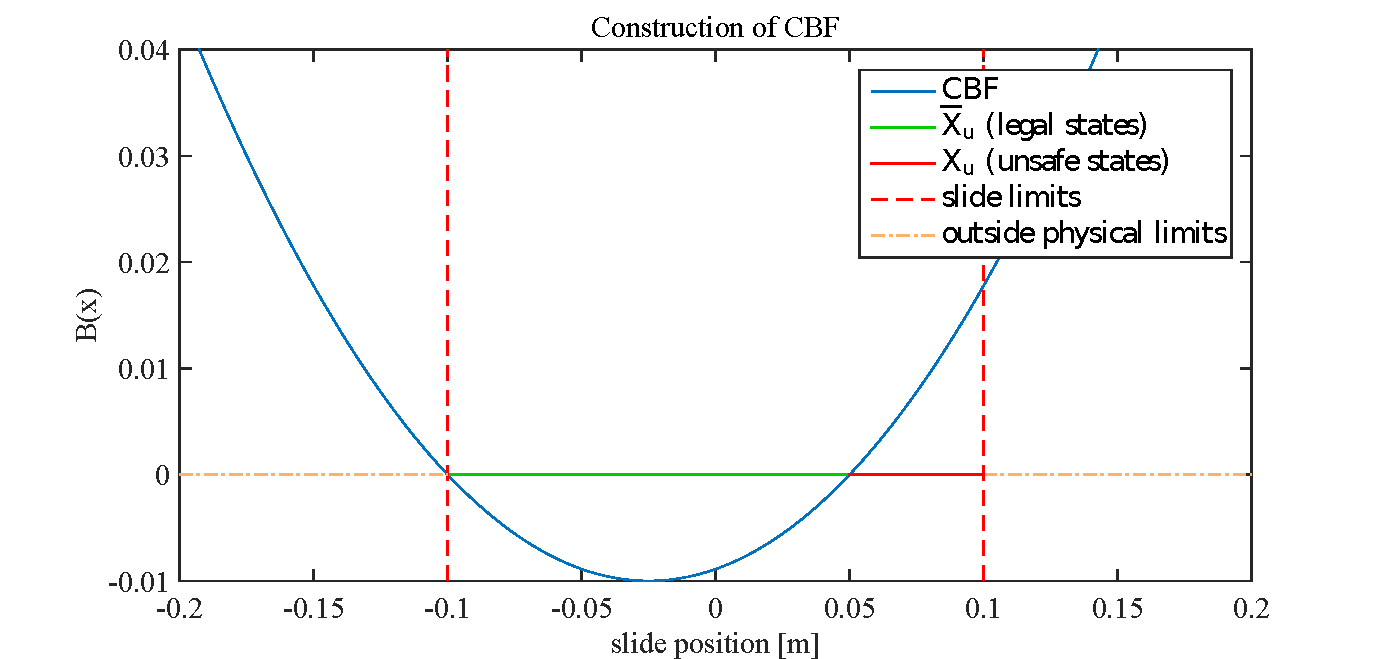
\includegraphics[scale=0.5]{parabel_1.pdf}
\caption{Barrier function along with the $\mathcal{X}_u$ and $\mathcal{X}_u^c$. Plot details and MATLAB script can be found in ????}
\label{fig:barrierfunction}
\end{figure}
\section{Controller Design}
A control laws is now introduced:
\begin{flalign*}
u(x) =
\begin{cases}
	\bar{N}\,x_\text{ref} - K\,x \kk &\text{if $x \in [\Psi_{s-}:\Psi_{s+}]$}\\
	 k_0(x)  \kk &\text{if $x \in [\Psi_{s+}:\Psi_{h+}] \mm \wedge \mm x \in [\Psi_{h-}:\Psi_{s-}]$}
\end{cases}
\end{flalign*}
This can be refined with a parameter $\sigma(x)$ such that the shift between the two control laws is not instantaneous \citep{bib:org_control}. Consider the control law below:
\begin{flalign*}
u(x) = \sigma(x)k_0(x)+(1-\sigma(x))\tilde{u}(x) = \sigma(x)k_0(x)+(1-\sigma(x))(\bar{N} \cdot x_\text{ref}-Kx) 
\end{flalign*}
\vspace{-0.8cm}
\begin{longtable}{p{.9\textwidth} p{.1\textwidth} p{.1\textwidth}} 
Where  & & \\
$u(x)$ is a control signal where safety is ensured  & [$\cdot$] \\
$\tilde{u}(x)$ is a control signal to the linear state space system such that $\tilde{u}=\bar{N}\cdot x_\text{ref}-Kx$ & [$\cdot$] \\ 
$k_0(x)$ is a control law that guarantees safety & [$\cdot$] \\ 
$\sigma(x)$ is a parameter that founds a linear combination between the two control inputs & [$\cdot$] \\ 
$K$ is a constant feedback matrix in $\mathbb{R}^{1 \times 1}$ & [$\cdot$] 
\end{longtable}
\vspace*{-0.2cm}
The control law is thereby a linear combination of two controllers. It is noted that:
\begin{flalign*}
\sigma(x) = 
\begin{cases}
0 \mm &\Rightarrow \mm \text{Pure control by pole placement, i.e. $u(x) = \tilde{u}(x) =  \bar{N}\cdot x_\text{ref}-Kx$ } \\
1 \mm &\Rightarrow \mm \text{Pure control for safety i.e. $u(x) = k_0(x)$ } \\
]0:1[ \mm &\Rightarrow \mm \text{A linear combination of the two control signals $u(x)$ and $\tilde{u}(x)$}
\end{cases}
\end{flalign*}
A block diagram is depicted in \autoref{fig:controlsystem}.
\begin{figure}[H]
	\center
		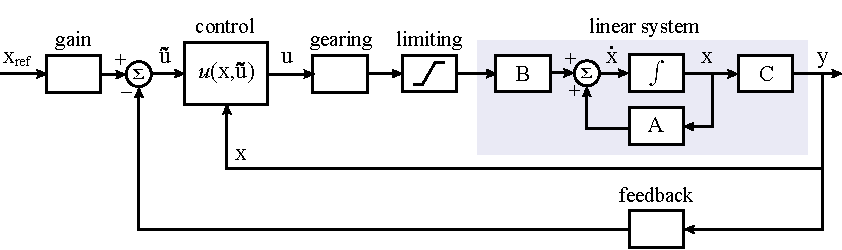
\includegraphics[scale=1]{control_system.pdf}
	\caption{Block diagram of the control system for slide position.}
	\label{fig:controlsystem}
\end{figure}
\subsection{Construction of $k_0$}
The control law ensuring safety can be found as \citep{bib:org_control}:
\begin{flalign}
k_0(x) = \begin{cases}
-\dfrac{L_fB(x)+ \sqrt{(L_fB(x))^2 + \kappa^2(L_gB(x))^TL_gB(x)}}{(L_gB(x))^TL_gB(x)}L_gB(x) &\text{if} \mm L_gB(x) \neq 0 \\
0  &\text{if} \mm L_gB(x) = 0
\end{cases}
\label{eq:control_law}
\end{flalign}
$\kappa$ is a design variable. High values of $\kappa$ implies increased aggressiveness. \Autoref{eq:control_law} ensures indeed safety for the closed loop system $\dot{x} = f_s(x)+g_s(x)k_0(x)$. This is easily proven as:
\begin{flalign*}
L_{f_{cl}}B(x) = L_fB(x) + L_gB(x)k_0(x)
\end{flalign*}
For $L_gB(x) \neq 0:$
\begin{flalign*}
L_{f_{cl}}B(x) &= L_fB(x) + L_gB(x) \left( -\dfrac{L_fB(x)+ \sqrt{(L_fB(x))^2 + \kappa^2(L_gB(x))^TL_gB(x)}}{(L_gB(x))^TL_gB(x)}L_gB(x) \right)  \\
&= L_fB(x) - (L_gB(x))^TL_gB(x) \dfrac{L_fB(x) - \sqrt{(L_fB(x))^2 + \kappa^2(L_gB(x))^TL_gB(x)}}{(L_gB(x))^TL_gB(x)}   \\ 
&= L_fB(x) - L_fB(x) - \sqrt{(L_fB(x))^2 + \kappa^2(L_gB(x))^TL_gB(x)} \\
&= - \sqrt{(L_fB(x))^2 + \kappa^2(L_gB(x))^TL_gB(x)} \mm \leq 0 \mm \forall \mm x
\end{flalign*}
As all terms within the square root are squared, no imaginary numbers occur, as a result $L_{f_{cl}}B(x) \leq 0$ 

According to \autoref{eq:control_law}, when $L_gB(x) = 0$:
\begin{flalign*}
L_{f_{cl}}B(x) = L_fB(x) + L_gB(x)\cdot 0 = L_fB(x)
\end{flalign*}
As $L_fB(x)$ is constructed such that $L_gB(x) = 0 \hspace{0.15cm} \Rightarrow \hspace{0.15cm} L_fB(x) < 0 $. 
\subsection{Construction of $K$ and $\bar{N}$}
No constraints to the constant feedback matrix $K$ will be outlined except stability. It will therefore be determined from the pole placement method such that:
\begin{flalign*}
p_d = 10\cdot \text{eig}(A) \kk \text{where \mm $A = -\tau_s^{-1}$}
\end{flalign*}
Ackermann's formula can be used \citep{bib:acker}.




\chapter[Controller Safety Verification with Putinar's Positivstellensatz]{Controller Safety Verification with \\Putinar's Positivstellensatz}\label{chap:putinar}  % Title in square brackets is what goes in TOC
\chaptermark{Controller Safety Verification with Putinar's Positivstellensatz} % Running footer, here we do not want a line break
	Barrier certificates can be used to (in)validate the safety compliance of a controller design by testing if a barrier certificate can be found according to \autoref{eq:barrier_constraints} for the closed-loop system $f_{cl}(x)$. When the vector field of the closed-loop system is polynomial and the sets $\mathcal{X}$, $\mathcal{X}_0$ and $\mathcal{X}_u$ are described by polynomial (in)equalities, a polynomial barrier certificate can be constructed using \gls{sos} optimization \citep{bib:prajna_framework}. A polynomial $p(x)$ is \gls{sos} if there exist polynomials $f_1,\dots,f_m$ such that \citep{bib:parrilo_sdp}
\begin{equation}
p(x) = \sum_{j=1}^{m}f_j^2(x)
\end{equation}

A \gls{sos} program is a convex optimization problem of the form \citep{bib:prajna_framework,bib:sostools}
\begin{subequations}
\begin{align}
&\min_{c}\, w^Tc\\
&\text{subject to} \qquad
q_{i,0}(x) + \sum_{j=1}^{m} q_{i,j}(x)g_j(x) \,\,\,\in \Sigma[x]
\qquad \text{for}\quad
i=1,\dots, p
\end{align}
\end{subequations}
\vspace*{-4mm}
\begin{tabular}{rl}
where &\\
$w$ & is a vector of weighting coefficients of the linear objective function\\
$c$ & is a vector formed by the (unknown) scalar real coefficients of $g_j(x)$\\
$g_j(x)$ & are polynomials in $x$\\
$q_{i,j}(x)$ & are given \gls{sos} polynomials with fixed coefficients\\
$\Sigma$ & denotes the set of \gls{sos} variables\\
$\mathbb{R}[x]$ &denotes a set of polynomials in $x$ with coefficients in $\mathbb{R}$\\
\end{tabular}\\\\


Introducing the notion of a monomial vector as a vector $Z$ in $x$ of degree $deg$; e.g. if $x\in\mathbb{R}^2$ and $deg=[0:2]$ each entry has the form $x_1^ax_2^b$ with exponents $a+b=deg=0,...,2$ i.e.
\begin{equation}
Z=[x_1^0x_2^0\quad x_1^1x_2^0\quad x_1^0x_2^1\quad x_1^1x_2^1\quad x_1^2x_2^0\quad x_1^0x_2^2]^T=[1\quad x_1\quad x_2\quad x_1x_2\quad x_1^2\quad x_2^2]^T
\end{equation} 
Now, according to \citep{bib:parrilo_sdp} a \gls{sos} polynomial $p\in \Sigma[x]$ can be formulated on a quadratic form comprising a coefficient matrix and a monomial vector
\begin{equation}
p = Z^T Q \, Z, \qquad\qquad p\geq 0 \quad \forall \, x\in\mathbb{R}^n %\setminus \{0\}
\label{eq:sos_polynomial}
\end{equation}
\begin{tabular}{rl}
where &\\
$Z$ & is a monomial vector in $x\in \mathbb{R}^n$\\
$Q$ & is a real positive semidefinite symmetric coefficient matrix\\
\end{tabular}\\

Now a polynomial barrier certificate can be constructed using Putinar's Positivstellensatz.
A Positivstellensatz is a structure theorem of a positive polynomial on some set, and gives an algebraic certificate that a solution exists for a system of real polynomial inequalities \citep{bib:positivstellensatz}. 
%Obtain certificates of positivity on a basic semialgebraic set $\mathbb{K}\subseteq\mathbb{R}^n$. \citep{bib:sos_putinar_laurent}
%A Positivstellensatz defines the regions of a semialgebraic set where a function is positive. 
%non-commutative Positivstellens\"{a}tze characterize things like a polynomial $p$ being positive where another polynomial $q$ is positive
Specifically for Putinar's Positivstellensatz, a compact set $\mathbb{K}$ is defined by the positivity of the polynomials $g_j$, e.g. in 1D Cartesian space $g(x)$ may be a parabola which is positive-valued on the interval $x\in[a,b]$, hence defining the semialgebraic set $\mathbb{K}=\{x\in[a,b]\}$.
Now the positivity (or nonnegativity or zero value) of a polynomial $h$ on the set $\mathbb{K}$ can be expressed in terms of a weighted sum of the polynomials $g_j$ with \gls{sos} coefficients \citep[pp 184-186]{bib:sos_putinar_laurent},\citep[pp 28-29]{bib:sos_putinar_lasserre}.\\

 

\begin{exa}[Putinar's Positivstellensatz]\label{def:putinar}
Given the finite family of polynomials $(g_j)_{j=1}^m$, the subset $Q(g)$ is called the quadratic module generated by the family $(g_j)$ \citep[p 29]{bib:sos_putinar_lasserre}
\begin{subequations}\label{eq:putinar}
\begin{align}
\text{polynomials} \qquad & (g_j)_{j=1}^m \in\mathbb{R}[x]\\
\text{set} \qquad & Q(g)=Q(g_1,...,g_m)\equiv\left\{\left.q_0+\sum\limits_{j=1}^{m}q_jg_j\,\,\right| \, (q_j)_{j=0}^m\in\Sigma[x]\right\}
\end{align}
\end{subequations}
Given a polynomial $h$ and a closed basic semialgebraic set $\mathbb{K}\subset\mathbb{R}^n$ defined by the nonnegativity of the polynomials $g_1,\dots, g_m$  
\begin{subequations}
\begin{align}
\text{polynomial} \qquad & h \in\mathbb{R}[x]\\
\text{set} \qquad & \mathbb{K}\equiv\left\{\left.x\in \mathbb{R}^n\,\, \right| \, (g_j)_{j=1}^m\geq0\right\}\qquad\qquad\qquad\qquad\qquad\quad
\end{align}
\end{subequations}
If the polynomial $h$ is strictly positive on the set $\mathbb{K}$, then $h\in Q(g)$, which means that $h$  can be formulated as
\begin{equation}\label{eq:sos_barrier}
h = q_0+\sum\limits_{j=1}^{m}q_jg_j
\end{equation}
\end{exa}


%\section{Using Sums of Squares to Construct a Barrier Certificate}
%\vspace*{-7mm}



In \autoref{def:putinar} the \gls{sos} variables $q$ are nonnegative per definition and as seen from \autoref{eq:sos_barrier} $h$ is positive on $\mathbb{K}$ as defined by $(g_j)_{j=1}^m$ being positive  in the region $\mathbb{K}$. Outside $\mathbb{K}$ one or more $g_j$s are negative, and hence the sign of $h$ cannot be determined outside $\mathbb{K}$.
Rearranging \autoref{eq:sos_barrier} to
\begin{equation}
q_0 = h - \sum _{j=1}^{m}q_jg_j \label{eq:putinar_sos}
\end{equation} 
however, the right-hand expression will always be nonnegative due to the SOS equality. Using the Matlab toolbox SOSTOOLS (see \autoref{app:sostools} for an introduction to the toolbox syntax), it is possible to solve for the unknown $h$ with a number of inequalities: expression $\in\Sigma[x]$ (corresponding to expression $\geq 0$) on each set $\mathbb{K}$. 

Now defining the semialgebraic sets $\mathcal{X}$, $\mathcal{X}_u$ and $\mathcal{X}_0$, is a matter of defining one or more functions $g_j$ for each set which are positive on the set. E.g. in order to define the region $\mathcal{X}$ construct a polynomial $g$ such that it is positive within the region and its zero level set constitute the desired border of the region. If several polynomials $g_j$ are used to define $\mathcal{X}$, the set is defined by the positive intersection region, i.e. where all of the $g_j$s are positive valued.

When the polynomials $g_j$ have been defined for each of the sets, the polynomial $h$ in \autoref{eq:putinar_sos} is substituted according to \autoref{def:barrier_certificate}, i.e. when defining $\mathcal{X}$ according to \autoref{cer3}, the polynomial $h$ can be written as $-dB/d x \, f_{cl}$; when defining $\mathcal{X}_0$ use $h=-B$ according to \autoref{cer1}; and when defining $\mathcal{X}_u$ use $h=B$ according to \autoref{cer2}.
In summary, referring to the requirements for a barrier certificate in \autoref{def:barrier_certificate} and the \gls{sos} formulation of the polynomial $h$ in \autoref{eq:putinar_sos} based on Putinar's Positivstellensatz, the inequalities defining the barrier certificate $B(x)$ can be set up as
\begin{subequations}\label{eq:barrier_constraints_putinar}
\begin{flalign}
&&	-B(x) &\geq 0 \kk  \forall \hspace{2mm} x \in \mathcal{X}_0 \qquad\quad \Leftarrow& 	-B(x) - \sum _{j=1}^{m}q_jg_j &\,\,\,\in \Sigma[x] &&& \label{cer1_putinar}\\
&&	B(x) \geq\epsilon&> 0 \kk  \forall \hspace{2mm} x \in \mathcal{X}_u \qquad\quad \Leftarrow& 	B(x)-\epsilon - \sum _{j=1}^{m}q_jg_j &\,\,\,\in \Sigma[x] &&&\label{cer2_putinar} \\
&&	-L_{f_{cl}}B(x) &\geq 0 \kk  \forall \hspace{2mm} x \in \mathcal{X} \qquad\quad\,\, \Leftarrow& 	-L_{f_{cl}}B(x) - \sum _{j=1}^{m}q_jg_j &\,\,\,\in \Sigma[x] &&& \label{cer3_putinar}
\end{flalign}
\end{subequations}
Note that the inequality is on positivity in \autoref{cer2} whereas it is on nonnegativity in \autoref{cer2_putinar}. By introducing an arbitrarily small $\epsilon>0$ the positivity constraint can be cast as the nonnegativity constraint in the  SOS inequality of \autoref{cer2_putinar}. %This is, however, not considered an issue in the scope of this project, as the position accuracy of the robot is not on the submillimeter level. 

\textcolor{red}{Bemærk, at denne sætning ikke siger hvor høj grad I skal vælge qerne. (husk at tænke på dette)}



 








 
	

\section{Defining a Polynomial Barrier Certificate in SOSTOOLS}\label{sec:app_sostools_barrier_search}

A polynomial barrier certificate can be constructed using \gls{sos} optimization, e.g by using a \gls{sos} program such as SOSTOOLS, which is a convex relaxation framework based on sum of squares decompositions of multivariate polynomials and semidefinite programming solvers \citep{bib:prajna_framework}. A short introduction to the SOSTOOLS syntax is presented in \autoref{app:sostools}.
Searching for a barrier certificate in SOSTOOLS require the definition of all of the vaiables and polynomials given by \autoref{eq:barrier_constraints_putinar} as follows:

\renewcommand{\labelitemii}{$\circ$}
\renewcommand{\labelitemiii}{$\bullet$}
\begin{itemize}
\itemsep-0.5mm
\item \textbf{Declare the Variables}\\
First declare the state space variables $x\in\mathbb{R}^n$ as \texttt{syms} or \texttt{pvar}, and initialize the SOS program with the system states.
\item \textbf{Define the Vector Field}\\
The open-loop state space system $f_{ol}(x)$ is defined, and a controller is found according to pole placement or another preferred method. Then write the closed-loop system equation $f_{cl}$ in terms of the symbolic state vector.
\item \textbf{Set up the Constraints on the Polynomial Barrier Certificate}\\
Declare a monomial vector $Z$ in $x$ (or part of $x$) of sufficiently large degree, and parametrize the polynomial $B(x)$ as a function of $Z$ with \texttt{sospolyvar}.  
The problem of finding the coefficients for the barrier certificate is now for each region $\mathcal{X}$, $\mathcal{X}_u$ and $\mathcal{X}_0$ a matter of defining the following:
\vspace*{-1mm}
\begin{itemize}
	\item \textbf{Define the Polynomials $g_j(x)$}\\
	Define one or more polynomials $g_j$ that are positive in the region to be defined and negative outside. Each polynomial may be solely a function of the robot tool position (and velocity) for static boundaries, and also a function of the heart position (and velocity) for dynamic boundaries. 
	\item \textbf{Declare the SOS Variables $q_j(x)$}\\
	Declare monomial vectors $Z_{q_j}$ in $x$ of appropriate degree (preferably as small as possible to keep the complexity of the problem as low as possible), and parametrize the SOS polynomials (multipliers) $q_j$ with \texttt{sossosvar}.
	\item \textbf{Set up the Inequality}\\
	Cf. the nonnegativity of an \gls{sos} polynomial ($q_0$), the \texttt{sosineq} can be written as the right-hand side of \autoref{eq:putinar_sos}: Choose a small positive number $\epsilon$ for defining the region $\mathcal{X}_u$;
	set up the inequality (corresponding to the region to be defined) according to \autoref{eq:barrier_constraints_putinar}. The inequality pertaining to a set may be defined in terms of several $g_j$s; if the set is defined by
	\begin{itemize}
		\item $g_1 \bigcap g_2 \bigcap ... \bigcap g_m$, then write $h - \sum q_jg_j\geq 0$
		\item $g_1 \bigcup g_2 \bigcup ... \bigcup g_m$, then write $h - q_1g_1\geq 0$, $h - q_2g_2\geq 0$ etc.
	\end{itemize} 
	Note that each expression in the inequalities of \autoref{eq:barrier_constraints_putinar} must have even degrees in the leading and trailing terms in order for the equality in \autoref{eq:putinar_sos} to hold.
\end{itemize}
\item \textbf{Solve the SOS Program}\\
With all inequalities defined in the program, SOSTOOLS is now ready to solve for the barrier certificate, if any certificate exists for the given system $f_{cl}(x)$. If no solution is found, increasing the degree of the \gls{sos} variables $q_j$ or the polynomial $B(x)$ may yield a solution. Otherwise it can be concluded that safety cannot be guaranteed of the closed-loop system under scrutiny. 
\end{itemize}





\textcolor{red}{Matter of defining degree of B and qs - how to decide?}
In the following section an example is given on how to search for a barrier certificate with SOSTOOLS.








%\textcolor{red}{Og hvordan bruger I så det. Kør eksemplet videre, så det er klart hvordan (8.2e) oversættes til SOS program. Jeg synes I skal køre eksemplet hele vejen igennem og idregne det i SOSTOOLS. På denne måde overbeviser i læseren og, at I kan oversætte teorien til praktisk implementation - Og dette giver points! }



\subsection{Example of Barrier Certificate Search with SOSTOOLS}
This section presents an example of a state $x\in\mathbb{R}$ controlling a 1D first order system robot $x_1$ corresponding to the slide joint being the only degree of freedom. First the system is defined, and a controller is designed with pole placement.
\begin{lstlisting}[language=matlab]
% Define state-space system with x1 = robot position
tau = 0.11; % time constant for the robot slide
A = -1/tau;
B = 1/tau;
k = place(A,B,[-10*1/tau]);
\end{lstlisting}
Then the symbolic state variables are declared for the SOS program, and the program is initialized.
\begin{lstlisting}[language=matlab]
% Declare state variables
pvar x1

% Initialize the sum of squares program
prog = sosprogram(x1);
\end{lstlisting}
%The reference for the robot position is generated as the 1D heart position, taking into account the system gain $\bar{N}$, and the closed-loop system equation is written as a function of the sybolic state. %\textcolor{red}{Something is wrong with the reference..?}
The vector field or derivative of the state can now be defined in terms on the symbolic state variable.
\begin{lstlisting}[language=matlab]
% Vector field dx/dt = fx (closed loop)
fx = (A-B*k)*x1;
\end{lstlisting}
For ease of defining a (1D) function $g$ that is positive on an interval [$p_1\,\,\, p_2$], a parabola function is used.
\begin{lstlisting}[language=matlab]
function [a,b,c] = parabola(p1,p2)
a = -1;
b = a*(p1^2-p2^2)/(p2-p1);
c = -a*p1^2-b*p1;
end
\end{lstlisting}
Now the region $\mathcal{X}$ can be defined for the slide region $\pm0.1$\,m using the Lie derivative inequality in \autoref{cer3}. The monomial degrees for $f$ and $B(x)$ are chosen as low as possible until a solution can be found. In this case a solution can be found for a degree of $B(x)$ that is 4.
\begin{lstlisting}[language=matlab]
% Define space X in R^n
[a,b,c] = parabola(-0.1,0.1); % get coefficients for parabola which is positive for x in [-0.1,0.1]
gX = a*x1^2+b*x1+c;
zX = monomials(vars,0:2);
[prog,qX] = sossosvar(prog,zX);
zB = monomials(x1,0:4);
[prog,Bx] = sospolyvar(prog,zB);
prog = sosineq(prog,-diff(Bx,x1)*fx-gX*qX);
\end{lstlisting}
Similarly, the region $\mathcal{X}_u$ is defined as the area between slide positions 5-10\,cm.
\begin{lstlisting}[language=matlab]
% Define space Xu in X
[a,b,c]=parabola(0.05,0.1);
gXu = a*x1^2+b*x1+c;
zXu = monomials(x1,0:2);
[prog,fXu] = sossosvar(prog,zXu);
prog = sosineq(prog,Bx-gXu*fXu);
\end{lstlisting}
And finally the region $\mathcal{X}_0$ is defined as $\mathcal{X}\setminus\mathcal{X}_u$.
\begin{lstlisting}[language=matlab]
% Define space X0 in X
[a,b,c] = parabola(-0.1,0.05);
gX0 = a*x1^2+b*x1+c;
zX0 = monomials(x1,0:2);
[prog,fX0] = sossosvar(prog,zX0);
prog = sosineq(prog,-Bx-gX0*fX0);
\end{lstlisting}
With all three areas defined according to \autoref{eq:barrier_constraints}, the program is ready to be solved. If a solution is found, an overview of the solution accuracy is printed in the Matlab terminal as the residual norm, number of iteration steps and solving time. To get the polynomial $B(x)$ use the function \verb|sosgetsol|.
\begin{lstlisting}[language=matlab]
% Solve for B
prog = sossolve(prog);
getB = sosgetsol(prog,Bx)
\end{lstlisting}
For this particular program, the solution barrier certificate is found to be
\begin{equation}
B(x) = 0.016168\cdot x_1^4 + 0.0064892\cdot x_1^3 + 0.00072547\cdot x_1^2 + 6.5473e\text{-}8\cdot x_1 - 2.7291e\text{-}6
\end{equation}
and is depicted in \autoref{fig:barrier_1storder_staticlim}.

\begin{figure}[htbp]
	\hspace*{-12mm}
	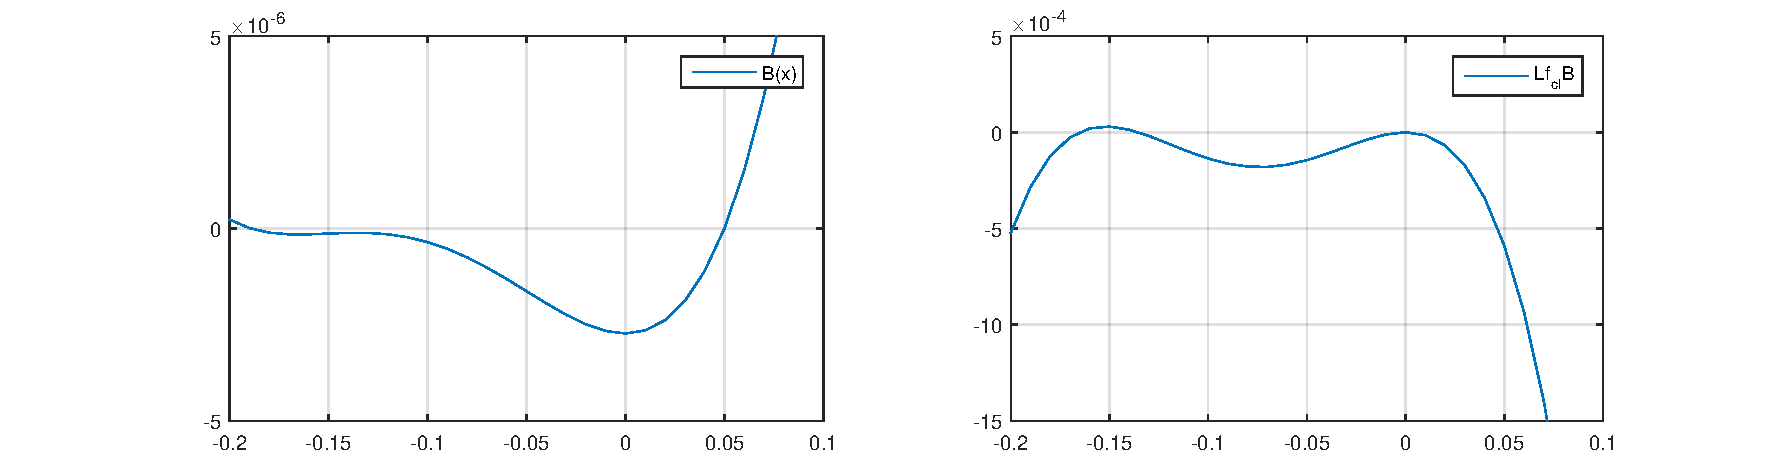
\includegraphics[width=1.1\textwidth]{1stordersys_staticlimits.pdf}
	\caption{A barrier certificate is found with SOSTOOLS that complies with the requirements in \autoref{eq:barrier_constraints}: it is positive on $\mathcal{X}_u=\{x_1\in [0.05,\,\,0.1]\}$ and negative on $\mathcal{X}_0=\{x_1\in [-0.1,\,\,0.05]\}$, and its Lie derivative is nonpositive on $\mathcal{X}=\{x_1\in [-0.1,\,\,0.1]\}$.}
	\label{fig:barrier_1storder_staticlim}
\end{figure}

\section{Approach for Verification of System Safety}

The following chapters present the safety verification of first- and second order systems in 1D and 3D with static and dynamic boundaries using Putinar's Positvstellensatz in the SOSTOOLS framework. The same systems are used for the analysis as in \autoref{part:cbf}, and to the extent it is possible, also the same (pole placement design) controllers are tested. \textcolor{red}{Correct this when the chapters are written!!!}



\chapter{Conclusion}\label{chap:conclusion}
This chapter will conclude on the results obtained throughout this thesis and put the solution and entire strategy into perspective in the discussion part.
\section*{Conclusion}
Safety aspects in robotic surgery and automated robotic surgery are found to be \textit{the} important factor, as analysed in \autoref{chap:intro}. Concurrently, it founds the basic framework in the long term goal of obtaining virtual fixtures. Consequently, a barrier certificate is stated in \autoref{chap:barrier_cerificates} which modifies and adapts the Lyapunov stability criteria to enable a way to define  safe and unsafe regions within the state-space. 

A theoretical controller is developed in \autoref{chap:cbf} based on control barrier functions which ensures that the  barrier certificate requirements presented in \autoref{chap:barrier_cerificates} are obeyed at all times. Thus, the control barrier function allows a way to ensure safety in real-time with astounding few calculations.

The control topology presented in \autoref{chap:cbf} is applied to three use cases which intend to commence a solution to the problem of guaranteeing safety in automated surgeries, i.e.:
\begin{itemize}
\item A concrete example of the use of control barrier functions is founded in \autoref{chap:cbf_1d_static}. It comprises the instrument slide movement. The system is modelled as both a first and second order system, thereby slowly increasing the complexity of the CBFs, such that necessary experience in the construction of CBFs can be gathered. The result is a successful controller guaranteeing safety by never entering predefined unsafe regions in one dimension for both a first and second order system approximation.
\item A safe regulator is designed to ensure system safety in relation to virtual fixtures in \autoref{chap:cbf_1d_dynamic}. A dynamic CBF is  constructed in accordance with the desire of virtual fixture and thus founds safety for operation on a beating heart. The result for this use case is that a safe distance between heart and robotic end effector can be set as desired.
\item Then safety considerations are extended to the 3D Euclidean space in \autoref{chap:cbf_3d_static} which implies additional implementation challenges such as a kinematic description (mapped and verified in \autoref{app:kinematic_model_robot}), forward kinematics and inverse kinematics. The construction of a CBF is taken to higher dimensions forming a barrier enclosing the interior of an ellipsoid, thus representing a heart or another vital organ fixed in space. The result is a valid CBF ensuring that the robot end effector is kept outside the ellipsoid at all time.
\end{itemize}
All three use cases are implemented in a simulation environment in MATLAB with convincing results, i.e. system safety is ensured by preventing the system state from entering specified unsafe regions. The controllers are furthermore implemented in C++ in the ROS (Robotic Operating System) framework. The ROS framework is founded in \autoref{app:ros} as a necessary condition to allow any implementation on the da Vinci robot. All development within ROS is tailored for this project and did not exist at project initiation. The implemented controllers comply with the expected outcome and do indeed behave as desired, i.e. ensuring safety by evading the predefined unsafe regions. Additionally, the implemented controllers are verified to require very little processing power making them ideal as real-time controllers.

The three use cases do, however, consist of simple models where the system order does not exceed 3. An important conclusion is drawn from the use cases, which already could be inferred from the one dimensional safe slide controller (developed in \autoref{chap:cbf_1d_static}) with system order 2. That is, for high order systems where the physical interpretation of the state vector is obscured, the construction of a valid CBF is a highly non-trivial task -- if not impossible. 

For this reason, the problem is turned upside down in \autoref{chap:putinar}, thus no restrictions are put forth in the controller development. Instead, the closed loop system is evaluated and the question is asked whether it complies with the barrier certificate requirement in \autoref{chap:barrier_cerificates}. The verdict is hereafter given as \textit{pass} or \textit{not pass}. For this purpose, \autoref{chap:putinar} presents the global SOS (Sum Of Squares) positivity characteristic and through Putinar's Positivstellensatz recast the barrier certificate formulation as a  problem of local positivity, thus allowing sets of unsafe and safe regions to be defined by unrestricted polynomials.

The strategy presented in \autoref{chap:putinar} is applied with the MATLAB toolbox SOSTOOLS in \autoref{chap:sostools} such that  barrier certificates can be searched for by automated means. Here, a framework is developed such that the toolbox takes a closed loop system description and a description of the safe and unsafe regions as inputs. The developed framework delivers an unambiguous certificate answering if the system is safe, thus constituting the \textit{pass} and \textit{not pass} verdict. The slide controller developed in \autoref{chap:cbf_3d_static} is accordingly taken as an example and the framework is verified with this example. Both the first and second order system approximation is analysed in the designed SOSTOOLS framework. It is, as expected, certified to be safe in almost the entire desired range.  These examples conclude and verify the use of the developed framework. The framework can easily handle other systems, as the task merely comprises other closed loop system descriptions as input in other dimensions with different safe and unsafe sets. This is a trivial task.

Hence, it can be concluded that the two initially desired strategies comprising the design and analysis of a safe controller are investigated and solved sufficiently to provide a "proof of concept" framework. This applies for both theory, simulation and implementation.


\section*{Discussion and Future Work}
The developed solution proves itself very efficient in both theory and simulation. However, the implementation aspect suffers from a number of issues which should be investigated in future work. This includes:
\begin{itemize}
\item Incorporate integral action in all controllers to eliminate steady state errors.
\item Increase the sampling rate from 100\,Hz to 2\,kHz which indeed is the long term goal. All controllers will draw benefits from this on the transition set $\mathcal{T}$. This may, however, introduce challenges as the allowed execution time (process time between every sample) is lowered to 0.5\,ms which is less than the actual execution time in \autoref{fig:3d_exe} for the safety controller in the 3D Euclidean space. Therefore, optimization must be performed in the implementation.
\item Improvement of the inverse kinematics solver as it occasionally chooses joint angles requiring multiple revolutions around the unit circle to obtain a position which could be reached with an angle less than $\pi$.
\end{itemize}
Additionally, the position controller already implemented on the FPGA (as seen in \autoref{fig:overview}), is left untouched. It may with removed to draw benefits from a more clear dynamics. This will require another system model, but may well be worth the trouble.

Furthermore, a consistently disregarded topic in this project is the use of trajectory planning. The controllers developed take only small steps as input. However, large step sizes have been given to the controllers in this project to demonstrate certain features, but obviously, it is desired to construct a trajectory planning layer taking the setpoints as input and breaking the path down into a sequence of adjacent points, thus ensuring that small step sizes are given to the controller.

Additionally, at no point  the orientation of the robot hand has been considered. Obviously, ensuring safety for the end effector is not sufficient as the heart or other vital organs can be penetrated or crushed by collision with the physical volume of the robotic tool other than the tip of the tool. This is an important topic in future work. Collision avoidance for the robotic parts themselves must also be studied when employing all four of the da Vinci arms in the setup, which is indeed the long term objective.

It is suggested for future use of the framework developed for barrier certificate search with SOSTOOLS to conduct the search in a more methodical manner by running the search like a Monte Carlo simulation, each time varying a parameter while keeping the others fixed. In this way the chance of determining a valid barrier function is maximized, thus indispensably invalidating system safety if no valid certificate can be found.

As explained by assistant nurse Jane Petersson in \autoref{sec:aau_doc}, there are veins, nerves and other organs which must not be cut during a surgery. It has been the aim to construct barrier certificates that can represent these parts of the body. However, it is clear that a realistic barrier certificate representing these parts is far away. Especially because they are time dependent and because, from time to time, the surgeon needs to move these parts to be able to operate in a certain area, thus reshaping these parts. Consequently, a very creative and adaptive barrier function is required and will as a necessary condition require robot vision (a continuous video stream analysis) such that these parts can be tracked. A way to resolve this complex problem of high dimensionality could be a combination of the design approach and analysis approach in the following way:
\vspace{-1.5mm}
\begin{enumerate}
	\itemsep-0.5mm
\item Search for a barrier certificate using the framework developed in \autoref{chap:sostools}.
\item Apply this barrier certificate as control barrier function in a similar way as done in \autoref{chap:cbf_1d_static}, \autoref{chap:cbf_1d_dynamic} and \autoref{chap:cbf_3d_static}.
\item Analyse the situation. Adjust the barrier certificate if necessary and describe the new closed loop system.
\item Take the new closed loop system as input to the framework developed in \autoref{chap:sostools} and start from 1 again.
\end{enumerate}
This iterative approach may along with the preceding listed bullet points get the robotic surgery industry one step closer to the end goal of guaranteed safe robotic surgery with the da Vinci robot,
which has been the sole application of the safety controllers derived throughout this project. However, it should take very little imagination to envisage that this way of constructing controllers has the potential to be used in many other industries where safety is critical or simply where regions are desirable to be left untouched.

\begingroup
\raggedright
\clearpage
\addcontentsline{toc}{chapter}{Literature}
\bibliography{bibtex/litteratur}
\endgroup
\label{sourceliste}

\newpage

\begin{appendices}
\appendix
%\renewcommand{\appendixname}{Appendices}
\renewcommand{\appendixname}{Appendix}
\renewcommand{\appendixtocname}{Appendix}

\chapter{Attached CD}\label{app:cd}
   \section*{$\bullet$ MATLAB scripts}
   \section*{$\bullet$ Measurement Files}

\lstdefinestyle{ubuntu}
{
    backgroundcolor=\color{black},
    basicstyle=\scriptsize\color{green}%\ttfamily
}
\chapter{Interfacing da Vinci with ROS}\label{app:ros}
This appendix ought to give concrete knowledge to utilize the \gls{ros} environment wrt. the \gls{daVinci} surgery robot at Aalborg University as it comprises an immense load of files, packages and various GUI interfaces. It also intends to provide an overview of the code structure and the underlying thoughts. The \gls{ros} environment is currently only developed for Ubuntu. The content of this appendix is accordingly assuming Ubuntu as operating system and assumes additionally basic knowledge in Unix. 

To install ROS on a private laptop, it is recommended to simply follow the below URL:

\hspace{1cm} {\color{blue}{\textit{http://wiki.ros.org/ROS/Installation}}}

Once ROS is installed, it is important to work on the \texttt{surgery-srv.lab.es.aau.dk} computer. It is recommended to work directly on the server in the lab as it provides additional GUI applications such as rviz, but it is obviously more convenient to work from a private laptop. Connection can be established through \texttt{ssh}:

%\begin{lstlisting}[style=ubuntu]
\hspace{1cm} \texttt{\$ ssh <user>@surgery-srv.lab.es.aau.dk}
%\end{lstlisting}

To get started with everything, open a terminal and initialize a ROS workspace as:

\hspace{1cm} \texttt{\$ mkdir -p daVinci\_ws/src}

Then navigate to the source directory (\texttt{src}) and type:

\hspace{1cm} \texttt{\$ catkin\_init\_workspace}

This creates a number of necessary files and folders. The code located at the "Robotic Surgery Group - Aalborg University" must be copied/cloned to the \texttt{src} folder. %({\color{blue}{\textit{https://github.com/AalborgUniversity-RoboticSurgeryGroup/}}}).
The original environment (clean configuration) can be cloned with the following git terminal commands:\vspace{0.1cm}

\hspace{0cm} \texttt{\$ git clone https://github.com/AalborgUniversity-RoboticSurgeryGroup/davinci\_description}

\hspace{0cm} \texttt{\$ git clone https://github.com/AalborgUniversity-RoboticSurgeryGroup/davinci\_driver}

\hspace{0cm} \texttt{\$ git clone https://github.com/AalborgUniversity-RoboticSurgeryGroup/davinci\_moveit\_config}\vspace{0.2cm}

Each command copies a so called \gls{ros} package which initially are created by the \texttt{catkin\_create\_pkg} command. A "package" is simply the name convention for a chunk of software in \gls{ros}. The name and file structure of a package should follow a certain standard, i.e. the \gls{rep} (it is not just the packages which should follow the \gls{rep} standard, but in fact the entire ROS workspace). This ought to make it easier to share and reuse code. The code developed in this thesis obeys to a large extend the \gls{rep}s but exceptions may occur. 

The three packages used are in that sense:
\begin{itemize}
\item \texttt{davinci\_description}
\item \texttt{davinci\_driver}
\item \texttt{davinci\_moveit\_config}
\end{itemize}
The development branch, i.e. the result of the work undertaken in this project, can be cloned as:

\hspace{0cm} \texttt{\$ git clone <URL> ---branch develop} \ \ \ {\color{RoyalBlue}{\textit{\# Clone all three packages}}}


To build the entire environment, open a terminal, navigate to the root of the workspace (\texttt{daVinci\_ws/}) and type:

\hspace{1cm} \texttt{\$ catkin\_make}

This connects all executables and the environment should hereafter be ready for use.
\section{General structure of a ROS setup}
After the workspace is created (called \texttt{daVinci\_ws}), the packages are cloned and the environment is build, the overall code structure should look like the tree structure found below:

\vspace{0.5cm}

\begin{tikzpicture}[scale=1]
\Tree [.\color{blue}{\texttt{daVinci\_ws}}
  [.\color{blue}{\texttt{build}} \text{make files etc.} ]  [.\color{blue}{\texttt{devel}} lib/setup ]  
     [.\color{blue}{\texttt{src}} {\color{white}{m}}$\underset{\text{input to the CMake build system}}{\text{\color{ForestGreen}{\texttt{CMakeLists.txt}}}}${\color{white}{m}} [.\hspace{0.2cm}\text{package $1$}\hspace{0.2cm} $\cdots$ $\cdots$ ]
     [.\hspace{0.2cm}\text{package 2}\hspace{0.2cm} $\cdots$ $\cdots$ ] \hspace{0.2cm}$\cdots$\hspace{0.2cm}  [.\hspace{0.2cm}\text{package $n$}\hspace{0.2cm} $\cdots$ $\cdots$  ]   ] 
  ]
\end{tikzpicture}
  
\vspace{0.2cm}

Each package has a similar structure. While the content of each package may vary, they always have a file called \texttt{package.xml} and \texttt{CMakeLists.txt}, and often the structure shown below.

%\begin{tikzpicture}[scale=1]
\hspace{2.5cm}
\Tree [.\text{package $m$} \color{ForestGreen}{\texttt{CMakeLists.txt}} \color{ForestGreen}{\texttt{package.xml}} [.\color{blue}{\texttt{config}} $\cdots$ $\cdots$ ]  [.\color{blue}{\texttt{launch}} $\cdots$ $\cdots$  ] [.\color{blue}{\texttt{others}} $\cdots$ $\cdots$ ] $\cdots$ ]
%\end{tikzpicture}



%%%>
\begin{comment}
:Title: Simple graph
:Tags: Arrows;Diagrams;Graphs;Mathematics
:Author: Stefan Kottwitz
:Slug: graph

A simple example of a graph with straight and bend arrows and loops.
It has been posted as answer to the question
http://tex.stackexchange.com/q/45734/213 of Ichibann.

* Define styles for edges, arrows, and nodes
* Place the main nodes
* Draw edges with nodes for description
* Use options `loop` and `bend` for loops and bent edges
* Specify `left` and `right` for bend direction and node placement
\end{comment}

Before elaborating on the significance of these folders and files, it is to some extend important to have an overview of the general used terms in the \gls{ros} environment. Those terms are briefly mentioned in \autoref{ros:node_etc}. 
\begin{figure}[H]
\center
\begin{tikzpicture}[->,>=stealth',shorten >=1pt,auto,node distance=5.5cm,
  thick,main node/.style={circle,fill=blue!20,draw,font=\sffamily\Large\bfseries}]
  \node[main node] (1) {\small \text{rosnode 1}};
  \node[main node] (2) [right of=1] {\small \text{rosnode 2}};

  \path[every node/.style={font=\sffamily\small}]
    (1) 
         edge node [right] {\hspace{-1.3cm}$\overset{\text{\normalsize rostopic}}{\text{\color{black}{(communication)}}}$} (2)
      %  edge [bend right] node[left] {0.3} (2)
      %  edge [loop above] node {0.1} (1)
      %  edge [bend right] node[right] {0.2} (2)
    (2) %edge node [right] {} (1)
        %edge [loop right] node {0.6} (2)
        %edge [bend right] node[right] {0.2} (1)
        ;
\end{tikzpicture}
\caption{Coherence between rosnodes and rostopics. A node is simply a process that performs some computation/algorithm and a topic is the communication channel between two or more ROS nodes. Two often used terms in this context are to publish/subscribe to a topic. To "publish" means to send a message from a topic and one can decode the message by "subscribing" to a topic.}
\label{ros:node_etc}
\end{figure}
With a basic understanding of ROS nodes and topics, the generic content of the two required files (\texttt{CMakeLists.txt} and \texttt{package.xml}) and the often used \texttt{launch} folder can be elaborated in \autoref{tab:eleb}. Other folders and files like \texttt{src}, \texttt{config}, \texttt{include} and similar are indeed also often used. They all have the purpose to enhance overview. The name should to some extend be self explaining, e.g. the \texttt{config} folder includes configuration files for the da-Vinci robot, the \texttt{src} folder often includes C++ files used for algorithms designed for specific purposes etc.
\begin{table}[H]
\begin{tabularx}{\textwidth}{X X X}
\rowcolor{HeaderBlue} 
 \textbf{\texttt{CMakeLists.txt}} & \textbf{\texttt{package.xml}}& \textbf{launch} \\
Package/project description, \gls{catkin} version, specification of required packages (not ROS packages but packages to create CMake environment variables), catkin dependencies and definitions and the specification of catkin build targets (executables and library targets). 
%%
$^*$  & Also referenced as a package manifest. It provides information about the maintainer, version, package name (e.g. \texttt{davinci\_driver}) and author. It specifies build tool dependencies (for the package to build itself - typically only catkin), build dependencies (required packages at build time), run-time dependencies and test dependencies (not used).  $^{**}$ & The content of a launch folder is primary used to start a group of nodes with unique topics and/or parameters. They are executed by the \texttt{roslaunch} terminal command followed by package name and lastly the name of the launch file, i.e.:\newline \texttt{roslaunch <package name> <name of launch file>}. \\  \rowcolor{textBlue}
\end{tabularx}
	\caption{Brief explanation of the purpose of the most common used folder names in a package.\newline $^*$ \citep{bib:CmakeLists}, $^{**}$ \citep{bib:package}.} 
\label{tab:eleb}
\end{table}
\section{Specific File Structure of this Thesis}
Low level flowcharts and low level code decomposition may be found in ??? and is as such not treated in this section.

The package where most of the development in this thesis takes place is in the \texttt{davinci\_moveit\_config} package located in the \texttt{src} folder. To give some idea of the content and how the code is structured, the directory tree on the following page is provided. It shows merely the "interesting files" seen from a developers point of view. In reality, additionally files are present. 
\newpage
\renewcommand*\DTstylecomment{\rmfamily\color{gray}\textsc}
\renewcommand*\DTstyle{\ttfamily\textcolor{blue}}

\begin{figure}[H]
% to make comment:
% .4 davinci\_moveit\_config\DTcomment{Guillaume}.
\dirtree{%
.1 /...
.2 davinci\_ws. %\DTcomment{workspace folder, created by mkdir}.
.3 build. %\DTcomment{generated by catkin\_init\_workspace}.
%.4 \color{gray}{..}.
.4 \color{gray}{... all make-files}. %\DTcomment{generated by catkin\_init\_workspace}.
.3 devel. %\DTcomment{generated by catkin\_init\_workspace}.
%.4 \color{gray}{..}.
.4 \color{gray}{... all libraries and setup files}. %\DTcomment{generated by catkin\_init\_workspace}.
.3 src.
.4 \color{ForestGreen}{CMakeLists.txt}.
.4 davinci\_description. %\DTcomment{\underline{Package:} Physical sizes and rotation matrices}.
.5 \color{ForestGreen}{CMakeLists.txt}.
.5 config.
.6 \color{ForestGreen}{davinci.rviz}.
.5 launch.
.6 \color{ForestGreen}{demo.launch}.
.6 \color{ForestGreen}{visualize\_in\_rviz.launch}.
.5 meshes.
.6 \color{gray}{... all .stl files (used for the 3D model in rviz)}.
.5 \color{ForestGreen}{package.xml}.
.5 robots.
.6 \color{ForestGreen}{remote\_center\_manipulator.xacro}\hspace{0.2cm}\color{gray}{\# rotation matrices for the hand}.
.6 \color{ForestGreen}{davinci.xacro}\hspace{0.2cm}\color{gray}{\# assembles all xml macros}.
.6 \color{ForestGreen}{p4\_arm.xacro}\hspace{0.2cm}\color{gray}{\# rotation matrices for the arm}.
.6 instruments.
.7 \color{ForestGreen}{needle\_driver.xacro}\hspace{0.2cm}\color{gray}{\# rotation matrices for instrument}.
.6 \color{gray}{... + other xacro files}.
.4 davinci\_driver. %\DTcomment{\underline{Package:} Interface with the physical robot}.
.5 \color{ForestGreen}{CMakeLists.txt}.
.5 \color{ForestGreen}{dstp.json}.
.5 launch.
.5 src.  
.6 \color{ForestGreen}{davinci\_driver.cpp}\hspace{0.2cm}\color{gray}{\# ... TODO }.
.6 \color{ForestGreen}{ros\_driver.cpp}\hspace{0.2cm}\color{gray}{\# ... TODO }.
.6 \color{ForestGreen}{sbrio\_driver.cpp}\hspace{0.2cm}\color{gray}{\# ... TODO }.
.5 srv.
.6 \color{gray}{... various hard-coded names}.
.5 config.
.6 \color{ForestGreen}{davinci\_ip\_adresses.yaml}\hspace{0.2cm}\color{gray}{\# set IP for RIO primary/secondary board}.
.6 \color{ForestGreen}{p4\_hand\_controller.yaml}\hspace{0.2cm}\color{gray}{\# specify each controllable joint}.
.5 include.
.6 \color{gray}{... header files for davinci\_driver.cpp and sbrio\_driver.cpp}.
.5 libsjon.
.6 \color{gray}{... various libraries}.
.4 davinci\_moveit\_config. %\DTcomment{\underline{Package:} Trajectory planning}.
.5 \color{ForestGreen}{CMakeLists.txt}.
.5 config.
.6 \color{ForestGreen}{controllers.yaml}\hspace{0.2cm}\color{gray}{\# specifies each controllable joint}.
.6 \color{ForestGreen}{davinci.srdf}\hspace{0.2cm}\color{gray}{\# collision and group specification}.
.6 \color{ForestGreen}{fake\_controllers.yaml}\hspace{0.2cm}\color{gray}{\# simulation controller specification}.
.6 \color{ForestGreen}{joint\_limits.yaml}\hspace{0.2cm}\color{gray}{\# Acceleration, velocity and position limits}.
.6 \color{ForestGreen}{kinematics.yaml}\hspace{0.2cm}\color{gray}{\# Kinematic solver specification}.
.6 \color{ForestGreen}{ompl\_planning.yaml}\hspace{0.2cm}\color{gray}{\# path planning specification}. 	
.5 launch.
.6 \color{ForestGreen}{davinci\_moveit\_controller\_manager.launch.xml}\hspace{0.2cm}\color{gray}{}.
.6 \color{ForestGreen}{move\_group.launch}\hspace{0.2cm}\color{gray}{\# launch all essential drivers }.
.6 \color{ForestGreen}{setup\_assistant.launch}\hspace{0.2cm}\color{gray}{\# launch to generate essential moveit files}.
.6 \color{gray}{... + other launch files controlled by the setup assistant}.
.5 \color{ForestGreen}{package.xml}\hspace{0.2cm}\color{gray}{\# specification of moveit dependencies}.
.5 src.
.6 \color{ForestGreen}{MoveGroupInterface.cpp}\hspace{0.2cm}\color{gray}{\# main C++ interface}.
}
%\caption{Code structure in the ROS environment}
\end{figure}


%Be very sure to clone all three packages.
\subsubsection*{Setup of Low Level Control}
Before the communication between ROS and da Vinci may be considered, all low level PID controllers must run correctly and the RIO configuration must be performed. 

From the \texttt{aau86730} computer, launch the \texttt{p4\_primary\_Control} icon located on the desktop and connect \texttt{RT Single Board RIO (172.26.12.32)} by right clicking the icon and press connect. Subsequently, navigate to \texttt{p4\_prim\_control\_FPGA\_multichannel\_7\_FLOAT\_SPI\_5.vi} and open it. This launch a GUI comprising access to the seven low level controllers which are activated from the arrow in the upper left corner. The controller gains, setpoints, maximum step size and various calibration options are easily accessible from this GUI, though it should not be necessary to modify any of those. 

Be sure that the gearing factors are specified as follows:
\begin{table}[H]
\begin{tabularx}{\textwidth}{X X X X X X X}
\rowcolor{HeaderBlue} 
\scriptsize \textbf{Intrument Jaw Left} &\scriptsize  \textbf{Intrument Jaw Right} &\scriptsize  \textbf{Intrument Pitch} &\scriptsize  \textbf{Instrument Roll} &\scriptsize  \textbf{Instrument Slide} & \scriptsize   \textbf{Hand Pitch} &  \scriptsize\textbf{Hand Roll}\\
12 & 12 & 12.4 & 7.5 & 1340 & 200 & 200\\
\end{tabularx}
	\caption{Measured gearing factors. Gearing factors are measured such that $\pi$/4 from \gls{ros} corresponds to 45 degrees on the real robot.}
\label{tab:gearing}
\end{table}
To allow the ROS environment access to the full range of setpoints, launch \texttt{p4-control\_prim-main4.vi} and activate this GUI in a similar manner. This GUI acts merely as interface and offers no user options as such. All necessary setup before initiating ROS is at this point in time performed.
\subsubsection*{ROS}
It is important to notice that every time a new terminal is commenced it is important to source the bash file from the workspace, i.e.:

\hspace{1cm} \texttt{\$ source devel/setup.bash}

The following list of commands must be executed from the root of the workspace. It is first of all important to collect all \gls{node}s such that they are able to communicate with each other. Open a terminal and run:

\hspace{1cm} \textbf{1.} \ \ \ \texttt{\$ roscore} \ \ \ {\color{RoyalBlue}{\textit{\# Leave this running in the terminal}}}

Now, to secure the TCP/IP connection between ROS and the RIO board (Rx \& Tx of setpoints), launch the driver from a new terminal:

\hspace{1cm} \textbf{2.} \ \ \  \texttt{\$ roslaunch davinci\_driver davinci\_driver.launch} \ \ \ {\color{RoyalBlue}{\textit{\# Leave this running}}} 

To allow trajectory planning, link the OMPL (Open Motion Planning Library) to the system by running: 

\hspace{1cm} \textbf{3.a} \ \ \  \texttt{\$ roslaunch davinci\_moveit\_config move\_group.launch} \ \ \ {\color{RoyalBlue}{\textit{\# Leave this running}}} 

If a 3D GUI interface is desired, open a new terminal and launch:

\hspace{1cm} \textbf{3.b} \ \ \  \texttt{\$ roslaunch davinci\_bringup visualization.launch} \ \ \ {\color{RoyalBlue}{\textit{\# This opens rviz}}} 

Press the "add" button in \texttt{rviz} and add the "MotionPlanning" option to the panel where start and goal state can be specified. Hereafter, plan and execute the specified goal. This cause the arm of da Vinci to reach out for the specified goal state consisting of five joint angles.

To launch the C++ interface, which allows 3D setpoints (by the KDL inverse kinematic solver) and custom joint specification, open a terminal and type:

\hspace{1cm} \textbf{4} \ \ \  \texttt{\$ rosrun davinci\_moveit\_config MoveGroupInterfaceExecute} \ \ \ {\color{RoyalBlue}{\textit{}}} 

This executes a GUI which provides the following options:

FILL IN!????

\subsubsection*{Useful and Regularly used ROS Commands}
To build the entire environment, navigate to the root of the workspace and type:

\hspace{1cm} \textbf{$\bullet$} \ \ \  \texttt{\$ catkin\_make}% \ \ \ {\color{RoyalBlue}{\textit{\# read various state information from terminal output}}} 

The current joint position is per default broadcasted to the topic \texttt{joint\_states}. To subscribe to this topic, open a terminal and type:

\hspace{1cm} \textbf{$\bullet$} \ \ \  \texttt{\$ rostopic echo joint\_states} \ \ \ {\color{RoyalBlue}{\textit{\# read various state information from terminal output}}} 

\hspace{1cm} \textbf{$\bullet$} \ \ \  \texttt{\$ rostopic echo joint\_states/position[$n$]} \ \ \  {\color{RoyalBlue}{\textit{\# read joint state angle from the $n^\text{th}$ joint state}}} 

Obtain a list of the used kinematic solvers, open a terminal and type:

\hspace{1cm} \textbf{$\bullet$} \ \ \  \texttt{\$ rosparam list | grep kinematics} \ \ \ {\color{RoyalBlue}{\textit{\# read solvers from terminal}}} 

view to all active topics:

\hspace{1cm} \textbf{$\bullet$} \ \ \  \texttt{\$ rostopic list} \ \ \ {\color{RoyalBlue}{\textit{\# read topics from terminal}}} 

To create a \gls{urdf} file from the present xacro files, type the below command from the root of the workspace:

\hspace{1cm} \textbf{$\bullet$} \ \ \  \texttt{\$ rosrun xacro xacro.py src/davinci\_description/robots/davinci.xacro > <name>.URDF} %\ \ \ {\color{RoyalBlue}{\textit{\# URDF is created}}} 
%
\subsection*{Setup Assistant}
To run the setup assistant, open a terminal, navigate to the root of the workspace and type:

\hspace{1cm} \textbf{$\bullet$} \ \ \  \texttt{\$ roslaunch davinci\_moveit\_config setup\_assistant.launch} \ \ \ {\color{RoyalBlue}{\textit{\# GUI is launched}}} 

A GUI offering eight setup options will now be present. Load the current \texttt{davinci\_moveit\_config} package as it is shown in \autoref{fig:setup_assistant_init}. The content of the eight options will be explained in the below itemize as it is important that all options are configured correctly for the kinematic solver to work correctly.
\begin{enumerate}
\item \textbf{Start:} It is possible to specify a new configuration package. This should only be necessary to do once. Since the \texttt{davinci\_moveit\_config} package is cloned from the development branch, it is sufficient to edit the existing package by pressing the associated button while the path to \texttt{davinci\_moveit\_config} is specified correctly.
\begin{figure}[H]
	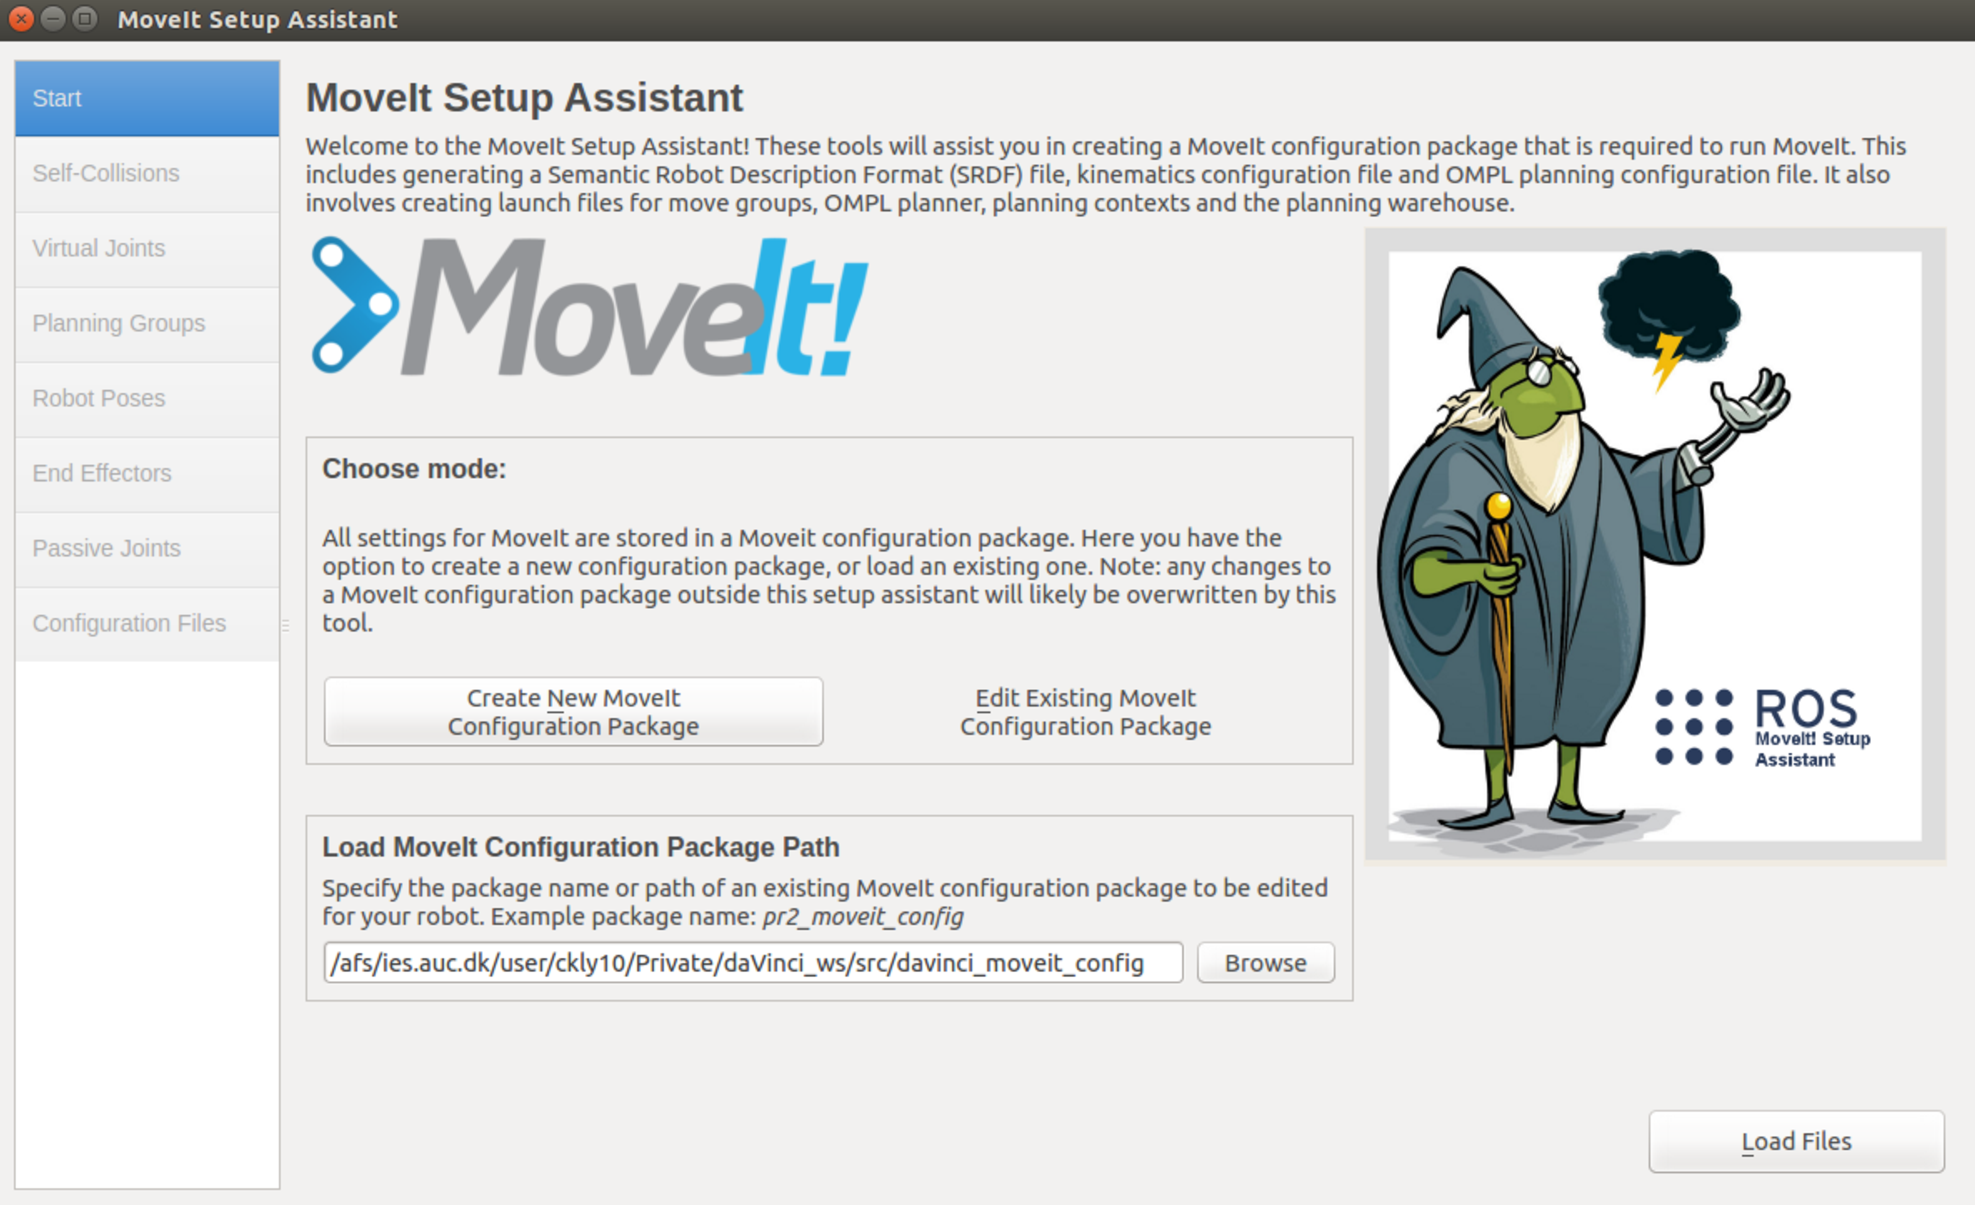
\includegraphics[scale=0.48]{setup_assistant}
	\caption{Welcome screen by the moveit setup assistant}
	\label{fig:setup_assistant_init}
\end{figure}
\item \textbf{Self Collision:}
This list is auto-generated from the associated xacro files specified in the \texttt{davinci\_} \texttt{description} package (from where a URDF file is generated and initially fed to the setup assistant). The default mode of operation disable collisions between adjacent links, links that can not physically collide, links that are always in collision and links that are in collision in the start-up mode. This is to enhance processing time \citep{bib:setup_assistant}. It is certainly possible to disable/enable collision between links as needed, though the default operation is used.	
\item \textbf{Virtual Joints:} It is here the robot is attached to the physical world by use of a virtual frame. Make sure the table is filled as shown:
\begin{table}[H]
\hspace{1cm}\begin{tabular}{l|l|l|l}
\textbf{Virtual Joint Name} & \textbf{Child Link}  & \textbf{Parent Frame}  & \textbf{Type}   \\
\hline
 \texttt{virtual\_joint} & \texttt{base\_link}  & \texttt{world}  &  \texttt{fixed} \\
\end{tabular}
\end{table}
\item \textbf{Planning Groups:} It is from here possible to describe the joints of the \texttt{p4\_arm} of da-Vinci. The Orocos \gls{kdl} kinematic solver seems to be dependent of at least six \gls{dof} (six active joints). It is possible to describe the arm by means of either joints, links or as a chain. It is chosen to describe the arm as joints. Be sure that a group \texttt{"gripper"} is added with the following kinematic specifications:
\begin{itemize}
\item Kinematic Solver: \texttt{kdl\_kinematic\_plugin/KDLKinematicPlugin}
\item Kin. Search Resolution: 0.005 (default)
\item Kin. Search Timeout (sec): 0.005 (default)
\item Kin. Solver Attempts: 3 (default)
\end{itemize}
It is furthermore important that it has the following joints specified:
\renewcommand*\DTstylecomment{\rmfamily\color{gray}\textsc}
\renewcommand*\DTstyle{\ttfamily\textcolor{black}} 
\begin{figure}[H]
\dirtree{%
.1 \textbf{\texttt{gripper}}. 
.2 joints.
.3 p4\_instrument\_slide - Prismatic.
.3 p4\_instrument\_roll - Revolute.
.3 p4\_hand\_pitch - Revolute.
.3 p4\_hand\_roll - Revolute.
.3 p4\_rcm\_instrument\_holder\_upper\_bar\_joint - Revolute.
.3 p4\_rcm\_upper\_bar\_base\_joint - Revolute.
.3 p4\_instrument\_jaw\_right - Revolute.
.2 Links \hspace{1cm}\color{gray}{\# Leave this empty}.
.2 Chain \hspace{1cm}\color{gray}{\# Leave this empty}.
.2 Subgroups \hspace{0.2cm}\color{gray}{\# Leave this empty}.
}
\end{figure}
This ensures that the group \texttt{gripper} can operate with six \gls{dof}. It is 
\item \textbf{Robot Poses:} It is from here possible to specify standard positions for the arm. The code developed during this thesis utilized a pose for an initial positions, hence be sure that a pose named \texttt{ready} is present under the group \texttt{gripper}. All joint states should be set to zero for this pose.
\item \textbf{End Effectors:} The end-effector is specified as shown:
\begin{table}[H]
\hspace{1cm}\begin{tabular}{l|l|l|l}
\textbf{End-Effector Name} & \textbf{Group Name}  & \textbf{Parent Link}  & \textbf{Parent Group}   \\
\hline
 \texttt{Gripper} & \texttt{gripper}  & \texttt{base\_link}  &  \texttt{--leave this empty--} \\
\end{tabular}
\end{table}
\item \textbf{Passive Joints:} A list of all joints will be available. It is important to specify the passive joints such that the \texttt{davinci\_moveit\_config} package know which joints are controllable. The table below shows how is must look:
\begin{table}[H]
\hspace{1cm}\begin{tabular}{l|l}
\textbf{Active joints} & \textbf{Passive Joints} \\
\hline
 \texttt{p4\_arm\_elevation} & \texttt{p4\_arm\_elevation} \\
  \texttt{p4\_arm\_yaw1} & \texttt{p4\_arm\_yaw1} \\
   \texttt{p4\_arm\_yaw2} & \texttt{p4\_arm\_yaw2} \\
    \texttt{p4\_arm\_yaw3} & \texttt{p4\_arm\_yaw3} \\
     \texttt{p4\_arm\_roll1} & \texttt{p4\_arm\_roll1} \\
      \texttt{p4\_arm\_yaw4} & \texttt{p4\_arm\_yaw4} \\
       \texttt{p4\_hand\_roll} & \texttt{p4\_rcm\_instrument\_holder\_upper\_bar\_joint} \\
        \texttt{p4\_hand\_pitch} & \texttt{p4\_rcm\_instrument\_bar\_joint} \\
          \texttt{p4\_rcm\_upper\_bar\_base\_joint} &  \\
   \texttt{p4\_rcm\_instrument\_holder\_upper\_bar\_joint} & \\
    \texttt{p4\_instrument\_slide} & \\
     \texttt{p4\_instrument\_roll} &  \\
      \texttt{p4\_instrument\_pitch} & \\
       \texttt{p4\_instrument\_jaw\_left} & \\
        \texttt{p4\_instrument\_jaw\_right} & \\
\end{tabular}
\end{table}
\item \textbf{Configuration Files:} The package will be generated from here by pressing the associated button. It is important to manually check out the files that should be generated. It is important to either recopy the below listed files to the package again or leave them apart from the setup assistant.
\begin{itemize}
	\item \texttt{src/davinci\_moveit\_config/launch/davinci\_moveit\_controller\_manager.launch}
	\item \texttt{src/davinci\_moveit\_config/config/controllers.yaml}
	\item \texttt{CMakeLists.txt}
	\item \texttt{package.xml}
\end{itemize}
It is finally of great significance to modify the \texttt{p4\_hand\_controller.yaml} file in the \texttt{davinci\_driver} package to include the correct joints. This should be taken care of when the development branch is cloned.
\end{enumerate}
%Files that needs to be created/modified manually when the setup assistant is launched:
\subsection*{Useful Debugging Commands}
To check which files are recently modified, open a terminal and run:

\hspace{1cm} \textbf{$\bullet$} \ \ \  \texttt{\$ find . -type f -exec ls -lt $\backslash$\{$\backslash$\} $\backslash$+ | head} 

This is fairly useful as, for example, the setup-assistant overwrites a number of files. 

{\color{white}{\gls{yaml}}}{\color{white}{\gls{xacro}}}



\chapter{Links and Joints 3D Overview}\label{app:links_joints_3d}
\begin{figure}[H]
	\center
		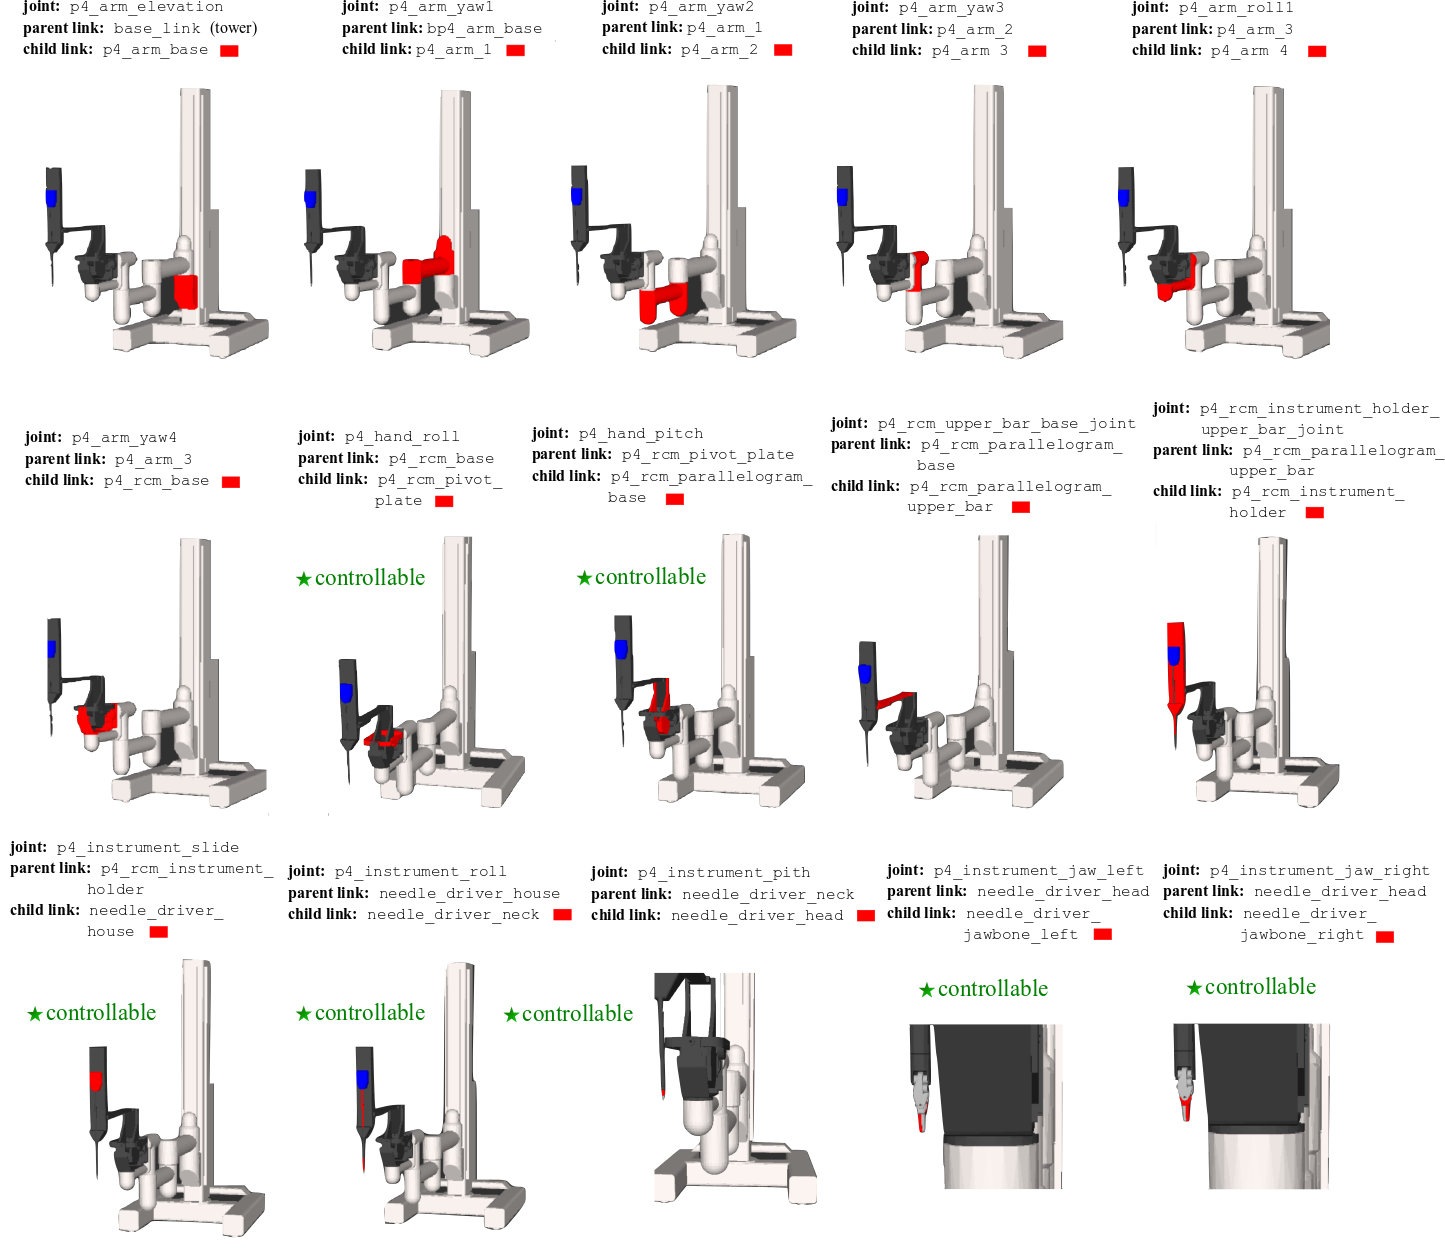
\includegraphics[width=1.2\textwidth, angle=270]{link_overview.png}
	\label{link_joint_overview}
\end{figure}

\chapter{Kinematic Models of the Robot}\label{app:kinematic_model_robot}
A rotation matrix $^a_b\mathbf{R}$ is an orthonormal matrix ($\mathbf{R}^{-1}=\mathbf{R}^T$) describing the rotation between two right-handed coordinate frames $\Psi_a$ and $\Psi_b$ such that any vector $^b\mathbf{v}$ (including $\Psi_b$ coordinate axes) given in the $\Psi_b$ frame can be "rotated" into $\Psi_a$ coordinates by the operation
\begin{equation}
^av =\, ^a_b\mathbf{R} \,\,^bv
\end{equation}
Note that the matrix $^a_b\mathbf{R}$ can also be seen as the rotation required of the frame $\Psi_a$ for it to coincide with $\Psi_b$.
Rotation of the frame $\Psi_a$ with an angle $\theta$ counterclockwise about a single axis (equal to clockwise "rotation" of the any vector in $\Psi_b$) correspond to the rotation matrices
\begin{small}
\begin{equation}
^a_b\mathbf{R}_x(\theta) = 
\begin{bmatrix}
1 & 0 & 0\\
0 & \cos\theta & -\sin\theta\\
0 & \sin\theta & \cos\theta
\end{bmatrix} 
\qquad
^a_b\mathbf{R}_y(\theta) = 
\begin{bmatrix}
\cos\theta & 0 & \sin\theta \\
0 & 1 & 0\\
-\sin\theta & 0 & \cos\theta
\end{bmatrix}
\qquad
^a_b\mathbf{R}_z(\theta) = 
\begin{bmatrix}
\cos\theta & -\sin\theta & 0\\
\sin\theta & \cos\theta & 0\\
0 & 0 & 1
\end{bmatrix}
\label{eq:RxRyRz}
\end{equation}
\end{small}
A sequence of rotations, transforming the vector $^cv$ given in the $\Psi_c$ frame to $\Psi_a$ coordinates, is implemented as
\begin{equation}
^a\mathbf{v} = \underbrace{^a_b\mathbf{R} \,\, ^b_c\mathbf{R}}_{^a_c\mathbf{R}} \,\,^c\mathbf{v} 
\end{equation}

The translation of the origin from the coordinate system $\Psi_a$ to $\Psi_b$ can be described by the position vector $^a_b\mathbf{p}$, which is a vector given in the $\Psi_a$ coordinate frame.
The relative configuration of two coordinate frames is their relative position and orientation, which can be expressed expressed by a homogeneous transformation matrix
\begin{equation}
^a_b\mathbf{T} = 
\begin{bmatrix}
^a_b\mathbf{R} & ^a_b\mathbf{p}\\
0 & 1
\end{bmatrix}
\end{equation}
The inverse of a configuration matrix is
\begin{equation}
^a_b\mathbf{T}^{-1} = 
\begin{bmatrix}
^a_b\mathbf{R}^T & -^a_b\mathbf{R}^T\,\,^a_b\mathbf{p}\\
0 & 1
\end{bmatrix}
\end{equation}
A sequence of configurations is implemented as
\begin{equation}
^a_n\mathbf{T} =\,\, ^a_b\mathbf{T} \,\, ^b_c\mathbf{T} \,\,...\,\, ^m_n\mathbf{T} = 
\begin{bmatrix}
^a_b\mathbf{R} \,\, ^b_c\mathbf{R} \,\,...\,\, ^l_m\mathbf{R} \,\,^m_n\mathbf{R} & ^a_b\mathbf{p} + ^a_b\mathbf{R} \,\, ^b_c\mathbf{p} + ... + (^a_b\mathbf{R}\,\, ^b_c\mathbf{R} \,\,...\,\, ^l_m\mathbf{R} \,\, ^m_n\mathbf{p} )\\
0 & 1
\end{bmatrix}
\end{equation}
where each matrix \gls{Tmtx} is a function of a rotation angle $\theta$ and a translation distance, which may be functions of time. \textcolor{white}{\gls{Rot} \gls{p_vec} \gls{alpha} \gls{beta} \gls{theta}}


\section{Existing Kinematics for the AAU da Vinci Robot}\label{sec:existing_kinematics}
The position of the end effector (the tip of the instrument) given in an inertial frame can be described as a sequence of joint rotations of the robot and the instrument, and translation from the inertial origin via the fixed-length links and the slide of the instrument.

A coordinate frame is defined for each degree of freedom, with origin on the axis of rotation. A set of coordinate frames and transformation matrices between the frames are given according to the \gls{ros} \texttt{xacro} files \texttt{tower}, \texttt{p4\_arm}, \texttt{remote\_center\_manipulator} and \texttt{needle\_driver}.

\begin{figure}[htbp]
\vspace*{-10mm}
\hspace{-10mm}
\subbottom[Coordinate frames for the joints on the robot arm.]{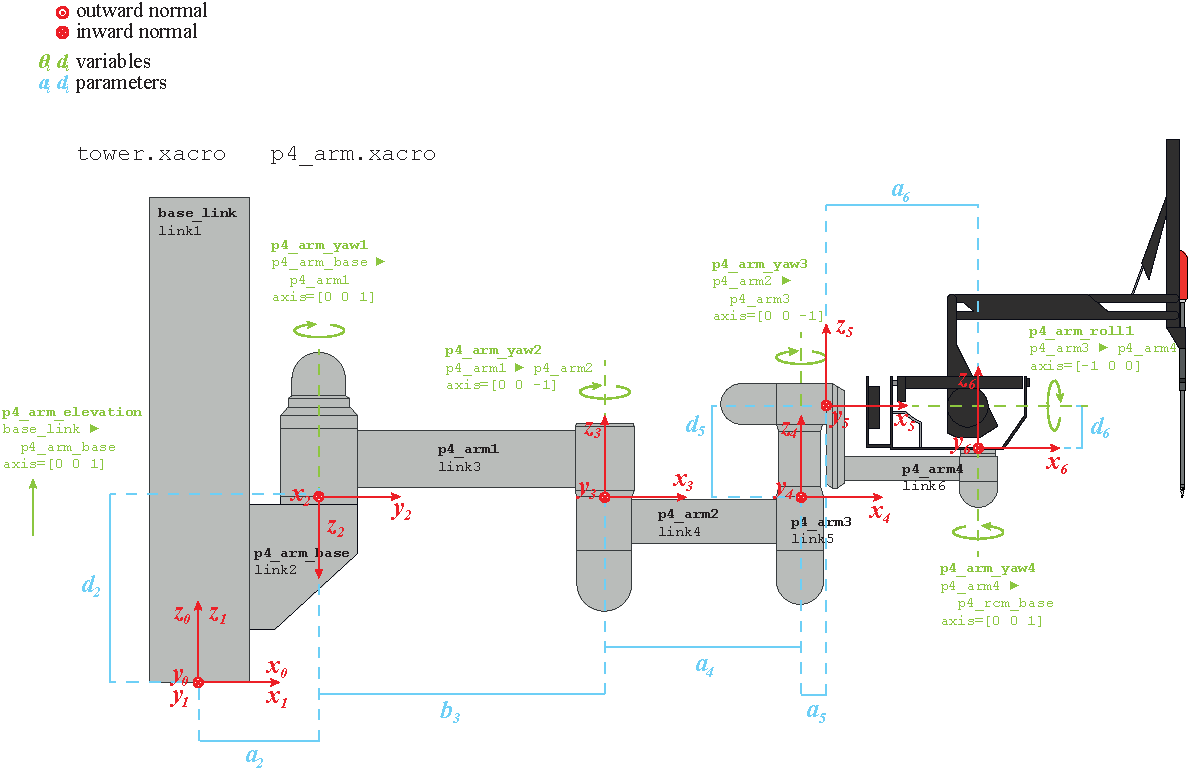
\includegraphics[width=1.1\textwidth]{p4_arm_xacro_frames.pdf}\label{fig:p4_arm_xacro_frames}}%
\vspace{5mm}\\
\hspace*{-15mm}
\subbottom[Coordinate frames for the joints on the robot hand and instrument.]{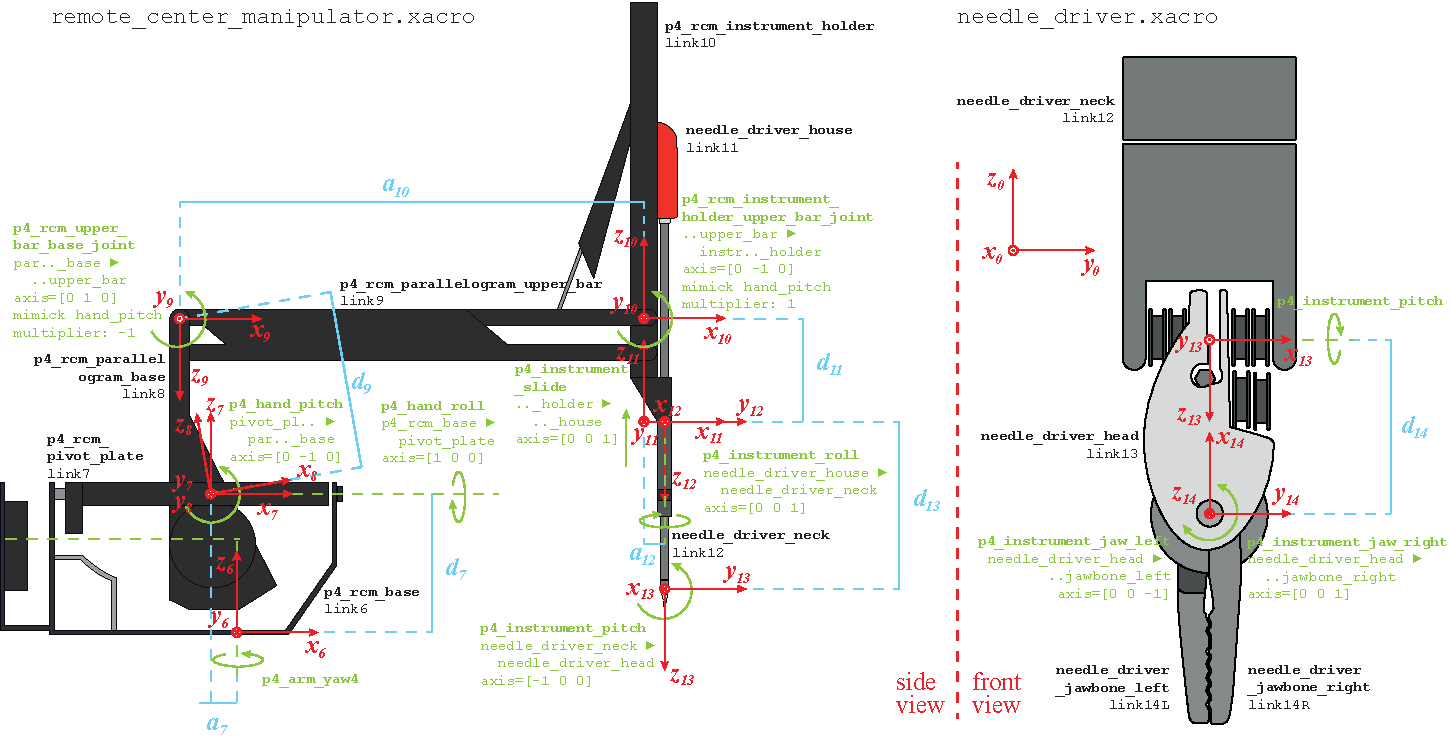
\includegraphics[width=1.15\textwidth]{p4_hand_xacro_frames.pdf}\label{fig:p4_hand_xacro_frames}}%
\caption{Orientation and position of coordinate frames $\Psi_0$, $\Psi_1$, ..., $\Psi_{14}$ according to the \gls{ros} \texttt{xacro} files.}
\label{fig:robot_xacro_frames}
\end{figure}

The position and orientation of the $i$th coordinate frame is given as a transformation matrix from the $i-1$th frame, where fixed distances and rotations are measured along/about the axes of the $i-1$th frame while free distances and rotations are measured along/about the axes of the $i$th frame. The parameters and variables shown in \autoref{fig:robot_xacro_frames} are given in \autoref{tab:xacro_param}.

\vspace{2mm}
\begin{table}[htbp]
\small
\centering
	\begin{tabular}{r | rrr c c l}\hline
		frame  & $a$ [m] & $b$ [m] & $d$ [m] & fixed rot. $\alpha$ [rad] & free rot. $\theta$ [rad] & name\\\hline
		1 & 0 & 0 & $d_1^*$ & $I$ & $I$ & \texttt{elevation}\\
		2 & 0.186 & 0 & 0.554 & $\textbf{R}_z(\pi/2)\textbf{R}_x(\pi)$ & $\textbf{R}_z(\theta_2^*)$ & \texttt{arm\_yaw1} \\
		3 & 0 & 0.583 & 0 & $\textbf{R}_z(\pi/2)\textbf{R}_x(-\pi)$ & $\textbf{R}_z(-\theta_3^*)$ & \texttt{arm\_yaw2} \\
		4 & 0.479 & 0 & -0.001 & $I$ & $\textbf{R}_z(-\theta_4^*)$ & \texttt{arm\_yaw3} \\
		5 & 0.057 & 0 & 0.198 & $I$ & $\textbf{R}_x(-\theta_5^*)$ & \texttt{arm\_roll1} \\
		6 & 0.352 & 0 & -0.117 & $I$ & $\textbf{R}_z(\theta_6^*)$ & \texttt{arm\_yaw4} \\
		7 & -0.042 & 0 & 0.161 & $I$ & $\textbf{R}_x(\theta_7^*)$ & \texttt{hand\_roll} \\
		8 & 0 & 0 & 0 & $\textbf{R}_y(-0.288)$ & $\textbf{R}_y(-\theta_8^*)$ & \texttt{hand\_pitch} \\
		9 & 0.011 & 0 & 0.186 & $\textbf{R}_y(0.288)\textbf{R}_x(\pi)$ & $\textbf{R}_y(-\theta_8)$ & \texttt{upper\_bar} \\
		10 & 0.520 & 0 & 0 & $\textbf{R}_x(\pi)$ & $\textbf{R}_y(-\theta_8)$ & \texttt{instrument\_holder} \\
		11 & 0 & 0 & -0.120 + $d_{11}^*$ & $I$ & $I$ & \texttt{instrument\_slide} \\
		12 & 0.052 & 0 & 0 & $\textbf{R}_z(\pi/2)\textbf{R}_x(\pi)$ & $\textbf{R}_z(\theta_{12}^*)$ & \texttt{instrument\_roll} \\
		13 & 0 & 0 & 0.177 & $I$ & $\textbf{R}_x(-\theta_{13}^*)$ & \texttt{instrument\_pitch} \\
		14L & 0 & 0 & 0.009 & $\textbf{R}_y(\pi/2)\textbf{R}_x(\pi/2)$ & $\textbf{R}_z(-\theta_{14L}^*)$ & \texttt{instrument\_jaw\_left} \\
		14\textbf{R} & 0 & 0 & 0.009 & $\textbf{R}_y(\pi/2)\textbf{R}_x(\pi/2)$ & $\textbf{R}_z(\theta_{14\textbf{R}}^*)$ & \texttt{instrument\_jaw\_right} \\
	\end{tabular}
	\caption{Variables (marked with $^*$) and parameters for the robot in \autoref{fig:robot_xacro_frames}. $I$ is the identity matrix (no rotation). Recent measures indicate that $d_2=0.812$, $a_2=0.198$, $a_4=0.435$, $\alpha_8=\textbf{R}_y(-0.07)$, $\alpha_9=\textbf{R}_y(0.07)\textbf{R}_x(\pi)$, $a_9=0$ and $d_\text{11,fixed}=0.188$ ($\Rightarrow$ $d_{12}=0.472$).}
	\label{tab:xacro_param}
\end{table}


I.e. according to \autoref{tab:xacro_param}, the transformation between frame 1 and 2 is given as:
\begin{equation}
^1_2\mathbf{T} = 
\begin{bmatrix}
\textbf{R}_z(\pi/2)\textbf{R}_x(\pi)\textbf{R}_z(\theta_2^*) & \mathbf{p}_2\\
0 & 1
\end{bmatrix}, \qquad\qquad
\mathbf{p}_2 = [0.186 \quad 0 \quad 0.554]^T
\end{equation}

The physical, low level controller and \gls{ros} limits for each of the variables are given in \autoref{tab:var_limits}

\vspace{2mm}
\begin{table}[htbp]
\small
\hspace*{-9mm}
%\begin{tabular}{l | cccccc}
%limits & $d_1^*$ & $\theta_2^*$ & $\theta_3^*$ & $\theta_4^*$ & $\theta_5^*$ & $\theta_6^*$ \\\hline
%physical & & & & & & \\
%\texttt{xacro} & [0, 1] & $\pm\pi/2$ & $\pm 2.8$ & $\pm 2.8$ & $\pm\pi/2$ & $\pm 2.8$
%\end{tabular}\\\\%
%\vspace{1mm}\\%
\begin{tabular}{l | ccccccc}\hline
limits & $\theta_7^*$ & $\theta_8^*$ & $d_{11}^*$ & $\theta_{12}^*$ & $\theta_{13}^*$ & $\theta_{14L}^*$ & $\theta_{14R}^*$ \\\hline
physical & $\pm$1.670 & [-0.951, 0.912] & [0.169, 0.410] & $\pm$4.712 & [-1.466, 1.536] & [-1.850, $\theta_{14\textbf{R}}^*$] & [$\theta_{14L}^*$, 1.702] \\
FPGA & [-1.333, 1.424] & [-0.812, 0.773] & [0.170, 0.409] & [-4.294, 4.416] & [-0.977, 0.908] & [-0.785, 1.335] & \\
\texttt{xacro} & $\pm\pi/2$ & [-0.8, 1] & $\pm$0.12 & $\pm3\pi/2$ & $\pm 1.5$ & $\pm 1.8$ & $\pm 1.8$
\end{tabular}
\normalsize
\caption{Limits on the (controllable) variables in \autoref{tab:xacro_param} and \autoref{fig:robot_xacro_frames}. The low level controller limits in the FPGA are set to avoid the physical limits, by switching off the motors on violation. The physical limits are measured limits.}
\label{tab:var_limits}
\end{table}
\vspace{2mm}

The first 6 degrees of freedom are elevation and rotation of the arm joints, and are manually set preoperatively and fixed, hence only the last 7 variables are controllable for trajectory planning. 
The frames are superimposed on the robot in \autoref{fig:robot_frames_pot}.

\vspace{-10mm}
\begin{figure}[htbp]
	\centering
\subbottom[\textbf{R}obot arm.]{\includegraphics[width=0.6\textwidth]{20150316_125233_red.pdf}\label{20150316_125233_red}}%
\hspace{5mm}
\subbottom[\textbf{R}obot arm.]{\includegraphics[width=0.25\textwidth]{20150316_125701_red.pdf}\label{20150316_125701_red}}%
\hspace{3mm}
\subbottom[\textbf{R}obot hand.]{\includegraphics[height=68mm]{20150316_140845_red.pdf}\label{20150316_140845_red}}%
\hspace{3mm}
\subbottom[Instr.]{\includegraphics[height=68mm]{20150317_110019_red.pdf}\label{20150317_110019_red}}%
\hspace{3mm}
\subbottom[Instr.]{\includegraphics[height=68mm]{20150317_111908_red.pdf}\label{20150317_111908_red}}%
\caption{Coordinate frame placement, distances and positive rotation direction for the robot arm, hand and instrument. In \autoref{20150316_125701_red} the positive rotation direction is shown for both \textbf{R}OS (green) and potentiometers (blue).}
\label{fig:robot_frames_pot}
\end{figure}

The position of the potentiometers measuring the joint variables 1-6 can be read from the interface to the secondary \gls{rio} as voltages. The scaling factor from these potentiometer voltages to the joint angle (in radians) are found through measurements and are given in \autoref{tab:arm_pot_factors}.
\vspace{2mm}
\begin{table}[H]
	\centering
\begin{tabular}{l | ccccc}
joint rotation [rad] & $\theta_2$, \texttt{yaw1} & $\theta_3$, \texttt{yaw2} & $\theta_4$, \texttt{yaw3} & $\theta_5$, \texttt{roll1} & $\theta_6$, \texttt{yaw4} \\
scaling factor [rad/V] & -0.225365326 & 0.302076216 & -0.306198114 & -0.311665937 & 0.314159265
\end{tabular}
\caption{Factor from potentiometer voltage measurements to arm joint angles.}
\label{tab:arm_pot_factors}
\end{table}



\newpage

\subsection{Testing Existing Kinematics in MATLAB}
MATLAB script and measurement files can be found in \autoref{app:cd} on the path \texttt{matlab\_scripts/kinematic\_ models/robot\_kinematics.m}.
The single-axis rotation matrices are defined according to \autoref{eq:RxRyRz}

\begin{lstlisting}[language=matlab]
function rotation = rot(axis,angle)
	if axis==1
		rotation = [1 0 0; 0 cos(angle) -sin(angle); 0 sin(angle) cos(angle)];
	elseif axis==2
		rotation = [cos(angle) 0 sin(angle); 0 1 0; -sin(angle) 0 cos(angle)];
	elseif axis==3
		rotation = [cos(angle) -sin(angle) 0; sin(angle) cos(angle) 0; 0 0 1];
	end
end
\end{lstlisting}

The parameters are set according to \autoref{tab:xacro_param} (corrected according to measurements, see \autoref{tab:arm_pot_factors}) and the transformation matrices are computed as follows

\begin{lstlisting}[language=matlab]
%% Existing reference frames according to xacro files

% parameters: distances [m], a: along x, b: along y, d: along z
a = [0.0 0.198 0.0 0.435 0.057 0.352 -0.052 0.0 0.0 0.430 0.0 0.052 0.0 0.0 0.0];
b = [0 0 0.583 0 0 0 0 0 0 0 0 0 0 0 0];
d = [0 0.812 0 -0.001 0.198 -0.117 0.161 0 0.186 0 -0.104 0.0 0.177 0.009 0.009];

% parameters: rotations [rad]
R = [eye(3) rot(3,pi/2)*rot(1,pi) rot(3,pi/2)*rot(1,-pi) eye(3) eye(3) eye(3) eye(3) rot(2,-0.1745) rot(2,0.1745)*rot(1,pi) rot(1,pi) eye(3) rot(3,pi/2)*rot(1,pi) eye(3) rot(2,pi/2)*rot(1,pi/2) rot(2,pi/2)*rot(1,pi/2)];
for i = 1:length(a)
	Rot(:,:,i) = R(:,(i-1)*3+1:i*3);
end

% -----------------------------------------------------------------------
% variables: actuation axes
ax = [3 3 -3 -3 -1 3 1 -2 2 -2 3 3 -1 -3 3];

% first make the variable rotation matrices (assume all variables are angles)
for i = 1:length(a)
	Rot_var(:,:,i) = rot(abs(ax(i)),sign(ax(i))*state(i));
end
% eliminating the two rotations where the variable is a distance
Rot_var(:,:,1) = eye(3);
Rot_var(:,:,11) = eye(3);

% making the variable translation vectors
for i = 1:length(a)
	for j = 1:3
		if i == 1 || i == 11
			if j == abs(ax(i)) 
				p(j,i) = sign(ax(i))*state(i);
			end
		else
			p(j,i) = 0;
		end
	end
end

% Transformation matrices (forward kinematics)
for i = 1:length(a)
	fixed = [Rot(:,:,i) [a(i) b(i) d(i)]'; zeros(1,3) 1];
	free = [Rot_var(:,:,i) p(:,i); zeros(1,3) 1];
	Trans(:,:,i) = fixed*free;
end
\end{lstlisting}

To test the accuracy of the defined kinematics, computed distances are compared to measured distances. The results are shown in \autoref{tab:xacro_distances}, for different state configurations, with state = [state$_\text{arm}$, state$_\text{hand}$] $= [\{d_1, \theta_2, \theta_3, \theta_4, \theta_5, \theta_6\}, \{\theta_7, \theta_8, d_{11}, \theta_{12}, \theta_{13}, \theta_{14L}, \theta_{14R}\}]$ (as $\theta_8=\theta_9=\theta_{10}$, 9 and 10 are left out).

\begin{table}[htbp]
\small
\setlength{\tabcolsep}{4pt}
\centering
\subbottom[]{%
\begin{tabular}{l r r}\hline
dist. & calc. & meas.\\\hline
$|\,^6_7 p|$ & 16.92 & 16\\
$|\,^6_8 p|$ & 16.92 & 16\\
$|\,^6_9 p|$ & 35.43 & 34\\
$|\,^6_{10} p|$ & 55.52 & 53\\
$|\,^6_{11} p|$ & 49.75 & 51\\
$|\,^6_{12} p|$ & 54.36 & 52\\
$|\,^6_{13} p|$ & 49.18 & 47\\
$|\,^6_{14} p|$ & 49.07 & 47\\\hline
%$\,^0_{14} p_x$ & 202.27 & 210.0\\
%$\,^0_{14} p_y$ & 0 & 0\\
%$\,^0_{14} p_z$ & 94.62 & 92.0
$|\,^0_{14} p|$ & 231.49 & 229
\end{tabular}
\label{tab:state0}%
}\hfill
\subbottom[]{%
\begin{tabular}{l r r}\hline
dist. & calc. & meas.\\\hline
$|\,^6_7 p|$ & 16.92 & 16\\
$|\,^6_8 p|$ & 16.92 & 16\\
$|\,^6_9 p|$ & 29.72 & 27\\
$|\,^6_{10} p|$ & 39.53 & 36\\
$|\,^6_{11} p|$ & 45.42 & 44\\
$|\,^6_{12} p|$ & 49.57 & 46\\
$|\,^6_{13} p|$ & 60.15 & 65\\
$|\,^6_{14} p|$ & 60.77 & 66\\\hline
%$\,^0_{14} p_x$ & 221.01 & 220\\
%$\,^0_{14} p_y$ & 0.81 & 25\\
%$\,^0_{14} p_z$ & 106.65 & 96
$|\,^0_{14} p|$ & 243.72 & 241
\end{tabular}
\label{tab:state5}%
}\hfill
\subbottom[]{%
\begin{tabular}{l r r}\hline
dist. & calc. & meas.\\\hline
$|\,^6_7 p|$ & 16.92 & 16\\
$|\,^6_8 p|$ & 16.92 & 16\\
$|\,^6_9 p|$ & 33.81 & 31\\
$|\,^6_{10} p|$ & 44.99 & 46\\
$|\,^6_{11} p|$ & 44.71 & 49\\
$|\,^6_{12} p|$ & 49.82 & 50\\
$|\,^6_{13} p|$ & 53.64 & 53\\
$|\,^6_{14} p|$ & 53.99 & 54\\\hline
%$\,^0_{14} p_x$ & 147.41 & 156\\
%$\,^0_{14} p_y$ & 30.52 & 42\\
%$\,^0_{14} p_z$ & 104.72 & 98
$|\,^0_{14} p|$ & 185.16 & 189
\end{tabular}
\label{tab:state6}%
}\hfill
\subbottom[]{%
\begin{tabular}{l r r}\hline
dist. & calc. & meas.\\\hline
$|\,^6_7 p|$ & 16.92 & 16\\
$|\,^6_8 p|$ & 16.92 & 16\\
$|\,^6_9 p|$ & 31.66 & 32\\
$|\,^6_{10} p|$ & 62.96 & 65\\
$|\,^6_{11} p|$ & 53.98 & 55\\
$|\,^6_{12} p|$ & 56.84 & 56\\
$|\,^6_{13} p|$ & 44.05 & 42\\
$|\,^6_{14} p|$ & 43.49 & 41\\\hline
%$\,^0_{14} p_x$ & 175.48 & 177\\
%$\,^0_{14} p_y$ & 42.04 & 53\\
%$\,^0_{14} p_z$ & 103.19 & 94
$|\,^0_{14} p|$ & 217.15 & 207
\end{tabular}
\label{tab:state7}%
}\hfill
\setlength{\tabcolsep}{6pt}
\caption{Calculated and measured distances [cm] between frame origins. In \ref{tab:state0} all variables are set to zero. In \ref{tab:state5} state$_\text{hand}=$[1.3, 0.7, -0.05, 0, 0, -0.23, 0]. In \ref{tab:state6} state = [\{0, 0.2, 0.5, -1.4, 0, 0.8\}, \{-0.5, 0.5, 0.03, 0, 0, -0.2, 0\}]. In \ref{tab:state7} state = [\{0, -0.2, -0.6, 0.9, 0, 0.4\}, \{-0.6, -0.6, 0, 0, 0, -0.2, 0\}].}
\label{tab:xacro_distances}
\end{table}

% % state 7


%\vspace*{-3mm}
\section{Defining Kinematics According to Denavit-Hartenberg Convention}\label{sec:denavit_hartenberg}
\vspace{-2mm}
In order to simplify calculations, the robot coordinate frame convention \gls{dh} is adapted, and a new set of coordinate frames and transformation matrices are established. According to the \gls{dh} convention a frame is placed such that
\begin{itemize}
\itemsep-1.3mm 
\item frame $i$ is fixed with respect to link $i$
\item the $z_i$ axis is aligned with link $i+1$ actuation axis
\item variable/parameter $\theta_i$ is the angle from $x_{i-1}$ to $x_i$ about $z_{i-1}$
\item variable/parameter $d_i$ is the distance from origin $i-1$ to $x_i$ measured along $z_{i-1}$
\item parameter $a_i$ is the distance from $z_{i-1}$ to $z_i$ measured along $x_i$
\item parameter $\alpha_i$ is the angle from $z_{i-1}$ to $z_i$ about $x_i$
\end{itemize}

Using this convention, all transformations between frames can be written on the form
\begin{equation}
\hspace*{-2mm}
\small
^{i-1}_i T = %T_{rot\,z,\theta_i} T_{trans\,z,d_i} T_{trans\,x,a_i} T_{rot\,x,\alpha_i} =
\begin{bmatrix}
\textbf{R}_z(\theta_i) & \begin{bmatrix}0\\ 0\\ d_i\end{bmatrix}\\
0 & 1
\end{bmatrix}
\begin{bmatrix}
\textbf{R}_x(\alpha_i) & \begin{bmatrix}a_i\\ 0\\ 0\end{bmatrix}\\
0 & 1
\end{bmatrix}
=
\begin{bmatrix}
\cos(\theta_i) & -\cos(\alpha_i)\sin(\theta_i) & \sin(\alpha_i)\sin(\theta_i) & a_i \cos(\theta_i)\\
\sin(\theta_i) & \cos(\alpha_i)\cos(\theta_i) & -\sin(\alpha_i)\cos(\theta_i) & a_i \sin(\theta_i)\\
0 & \sin(\alpha_i) & \cos(\alpha_i) & d_i\\
0 & 0 & 0 & 1
\end{bmatrix}
\end{equation}

The placement of coordinate frames according to the \gls{dh} convention is shown in \autoref{fig:robot_DH_frames} and the parameters used for this set of frame transformations are given in \autoref{tab:DH_param}.


\begin{figure}[htbp]
	\vspace*{-10mm}
	\hspace{-10mm}
	\subbottom[Coordinate frames for the joints on the robot arm.]{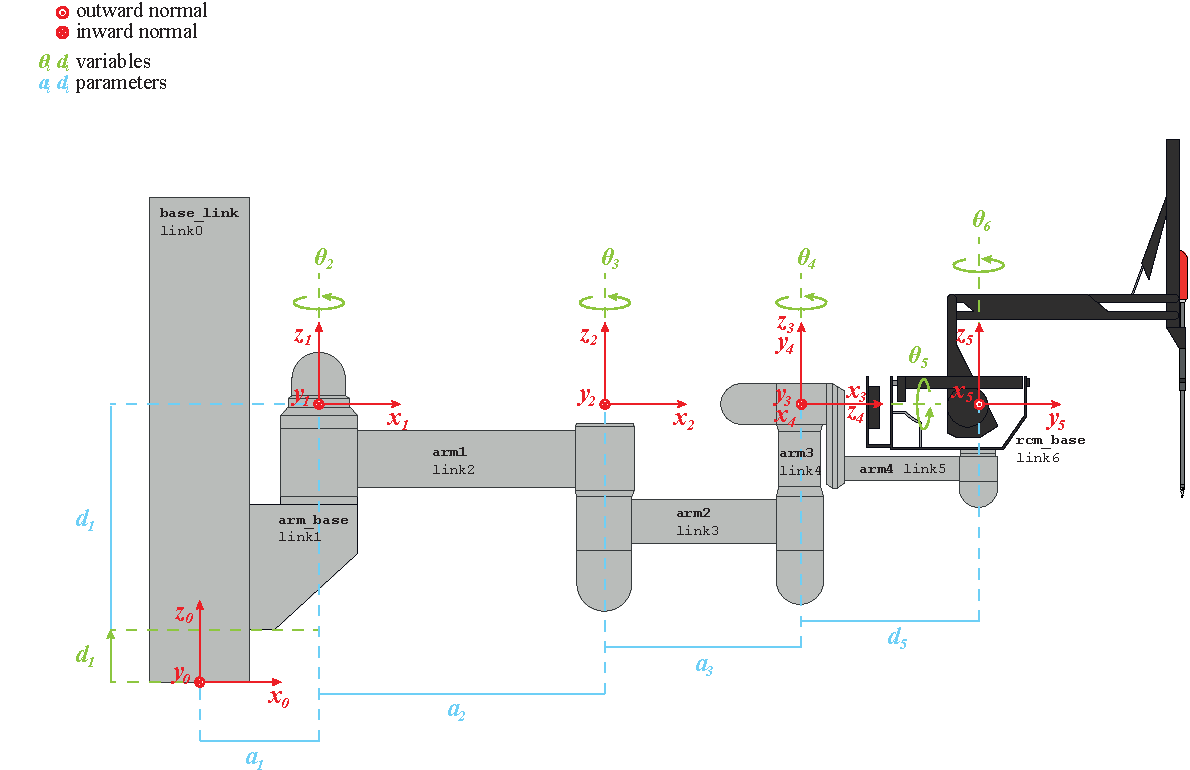
\includegraphics[width=1.1\textwidth]{p4_arm_DH_frames.pdf}\label{fig:p4_arm_DH_frames}}%
	\vspace{5mm}\\
	\hspace*{-15mm}
	\subbottom[Coordinate frames for the joints on the robot hand and instrument.]{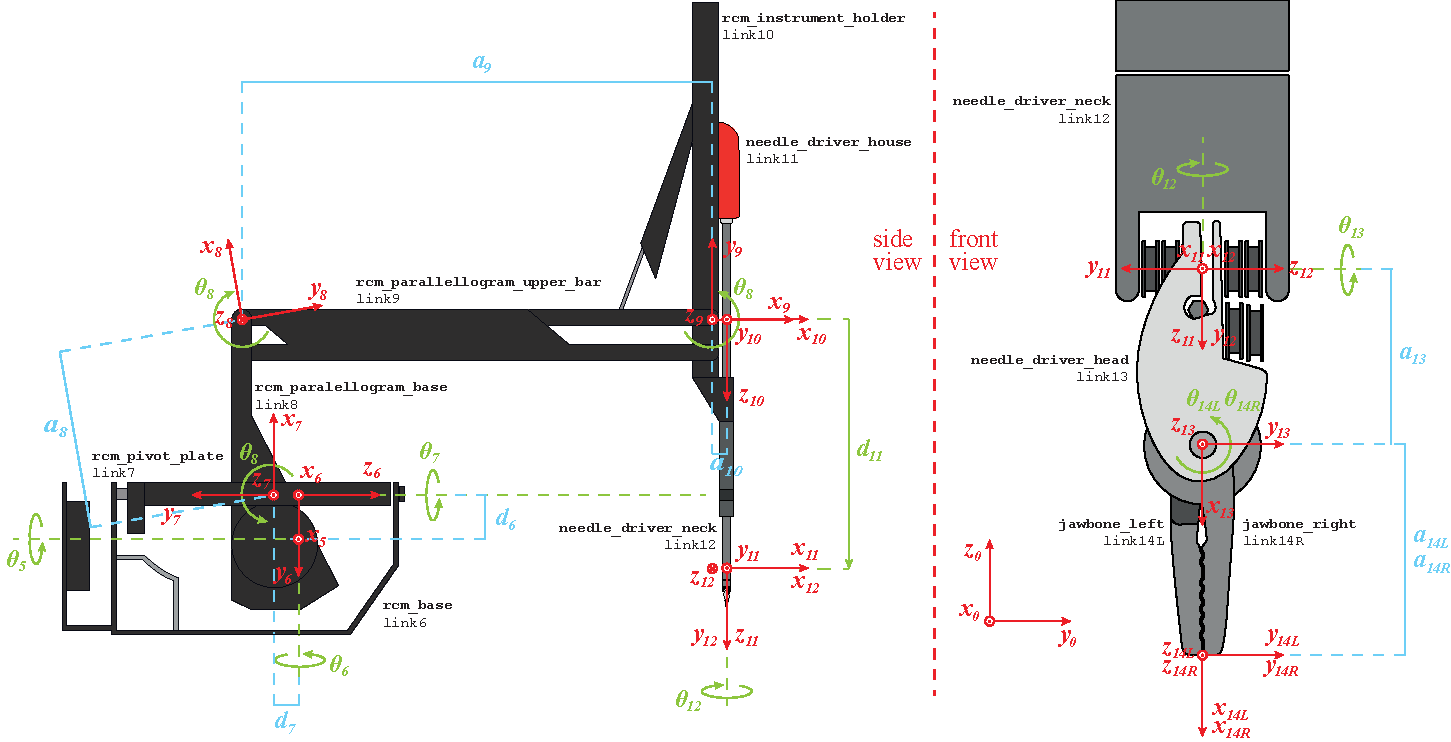
\includegraphics[width=1.15\textwidth]{p4_hand_DH_frames.pdf}\label{fig:p4_hand_DH_frames}}%
	\caption{Orientation and position of coordinate frames $\Psi_0$, $\Psi_1$, ..., $\Psi_{14}$ defined according to the \gls{dh} convention.}
	\label{fig:robot_DH_frames}
\end{figure}

\begin{table}[htbp]
	\small
	\vspace*{-3mm}
	\centering
	\begin{tabular}{r | rrrr}\hline
		$i$  & $\theta_i$ [rad]& $d_i$ [m] & $a_i$ [m] & $\alpha_i$ [rad] \\\hline
		1 & 0 &  $0.453+d_1^*$ & 0.198 & 0 \\
		2 & $\theta_2^*$ & 0 & 0.582 & 0 \\
		3 & $\theta_3^*$ & 0 & 0.435 & 0\\
		4 & $\pi/2+\theta_4^*$ & 0 & 0 & $\pi/2$\\
		5 & $\pi+\theta_5^*$ & 0.412 & 0 & $\pi/2$ \\
		6 & $\theta_6^*$ & 0.047 & 0 & $-\pi/2$ \\
		7 & $-\pi/2+\theta_7^*$ & -0.035 & 0 & $-\pi/2$ \\
		8 & $0.03+\theta_8^*$ & 0 & 0.190 & $\pi$ \\
		9 & $0.03+\pi/2+\theta_8^*$ & 0 & 0.515 & $\pi$ \\
		10 & $\theta_8^*$ & 0 & 0.040 & $\pi/2$\\
		11 & 0 & $0.282+d_{11}^*$ & 0  & 0 \\
		12 & $\theta_{12}^*$ & 0 & 0 & $\pi/2$ \\
		13 & $\pi/2+\theta_{13}^*$ & 0 & 0.009 & $\pi/2$ \\
		14L & $\theta_{14L}^*$ & 0 & 0.009 & 0\\
		14R & $\theta_{14R}^*$ & 0 & 0.009 & 0 \\
	\end{tabular}
	\caption{Variables (marked with $^*$) and parameters for the robot in \autoref{fig:robot_DH_frames} defined according to the \gls{dh} convention, where $\theta_i$ and $d_i$ are rotation/translation along $z_{i-1}$, while $a_i$ and $\alpha_i$ are translation/rotation along $x_i$.}
	\label{tab:DH_param}
\end{table}

\subsection{Testing \gls{dh} Kinematics in MATLAB}
The new transformation matrices are computed and tested similarly, to determine the accuracy of the defined robot kinematics, and the results are seen in \autoref{tab:DH_distances}.
MATLAB script and measurement files can be found in \autoref{app:cd} on the path \texttt{matlab\_scripts/kinematic\_models/robot\_kinematics.m}.
\begin{lstlisting}[language=matlab]
%% Coordinate frames defined according to Denavit-Hartenberg convention
% Parameters
a_fix = [0.198 0.5820 0.435 0 0 0 0 0.1900 0.515 0.0400 0 0 0.0095 0.0095 0.0095];
d_fix = [1 0 0 0 0.4122 0.0474 -0.0450 0 0 0 0.282 0 0 0 0];
alpha = [0 0 0 pi/2 pi/2 -pi/2 -pi/2 pi pi pi/2 0 pi/2 pi/2 0 0];
theta_fix = [0 0 0 pi/2 pi 0 -pi/2 10/180*pi 10/180*pi+pi/2 0 0 0 pi/2 0 0];

% Variables (signs are included as long as state comes from old frame convention)
d_free = [d1 0 0 0 0 0 0 0 0 0 -d11 0 0 0 0];
theta_free = [0 -th2 -th3 -th4 -th5 th6 th7 th8 th8 th8 0 th12 -th13 th14L -th14R];

% Transformation matrices
for i = 1:length(a_fix)
	Tz = [rot(3,theta_free(i)+theta_fix(i)) [0;0;d_free(i)+d_fix(i)]; zeros(1,3) 1];
	Tx = [rot(1,alpha(i)) [a_fix(i);0;0]; zeros(1,3) 1];
	T_DH(:,:,i) = Tz*Tx;
end
\end{lstlisting}

\begin{table}[htbp]
\small
\setlength{\tabcolsep}{4pt}
\centering
\subbottom[]{%
\begin{tabular}{l r r}\hline
dist. & calc. & meas.\\\hline
$|\,^5_6 p|$ & 4.74 & 5\\
$|\,^5_7 p|$ & 6.54 & 7\\ %6\\
$|\,^5_8 p|$ & 24.71 & 24\\
$|\,^5_9 p|$ & 49.60 & 49\\
$|\,^5_{10} p|$ & 53.15 & 53\\ %52\\
$|\,^5_{11} p|$ & 47.94 & 48\\
$|\,^5_{12} p|$ & 47.94 & 48\\
$|\,^5_{13} p|$ & 48.04 & 48\\
$|\,^5_{14} p|$ & 48.16 & 48\\\hline
%$\,^0_{14} p_x$ & 210.42 & 210\\
%$\,^0_{14} p_y$ & 0 & 0\\
%$\,^0_{14} p_z$ & 93.35 & 92
$|\,^0_{14} p|$ & 230.20 & 229
\end{tabular}
\label{tab:state0dh}%
}\hfill
\subbottom[]{%
\begin{tabular}{l r r}\hline
dist. & calc. & meas.\\\hline
$|\,^5_6 p|$ & 4.74 & 5\\ %4\\
$|\,^5_7 p|$ & 6.54 & 7\\ %8\\
$|\,^5_8 p|$ & 23.79 & 24\\ %20\\
$|\,^5_9 p|$ & 35.40 & 34\\ %33\\
$|\,^5_{10} p|$ & 39.20 & 39\\ %49\\
$|\,^5_{11} p|$ & 57.82 & 64\\ %66\\
$|\,^5_{12} p|$ & 57.82 & 64\\ %66\\
$|\,^5_{13} p|$ & 58.54 & 67\\ %65\\
$|\,^5_{14} p|$ & 59.23 & 68\\ \hline %66\\
%$\,^0_{14} p_x$ & 230.81 & 220\\
%$\,^0_{14} p_y$ & 1.88 & 25\\
%$\,^0_{14} p_z$ & 107.03 & 96
$|\,^0_{14} p|$ & 243.20 & 241
\end{tabular}
\label{tab:state5dh}%
}\hfill
\subbottom[]{%
\begin{tabular}{l r r}\hline
dist. & calc. & meas.\\\hline
$|\,^5_6 p|$ & 4.74 & 5\\ %6\\
$|\,^5_7 p|$ & 6.54 & 7\\ %8\\
$|\,^5_8 p|$ & 25.14 & 24\\ %19\\
$|\,^5_9 p|$ & 39.04 & 40\\ %37\\
$|\,^5_{10} p|$ & 43.02 & 42\\ %41\\
$|\,^5_{11} p|$ & 51.33 & 51\\ %54\\
$|\,^5_{12} p|$ & 51.33 & 51\\ %54\\
$|\,^5_{13} p|$ & 51.86 & 52\\ %55\\
$|\,^5_{14} p|$ & 52.40 & 52\\\hline %55\\
%$\,^0_{14} p_x$ & 150.05 & 156\\
%$\,^0_{14} p_y$ & 39.71 & 42\\
%$\,^0_{14} p_z$ & 103.79 & 98
$|\,^0_{14} p|$ & 184.99 & 189
\end{tabular}
\label{tab:state6dh}%
}\hfill
\subbottom[]{%
\begin{tabular}{l r r}\hline
dist. & calc. & meas.\\\hline
$|\,^5_6 p|$ & 4.74 & 5\\
$|\,^5_7 p|$ & 6.54 & 7\\ %8\\
$|\,^5_8 p|$ & 21.65 & 22\\ %24\\
$|\,^5_9 p|$ & 58.87 & 58\\ %56\\
$|\,^5_{10} p|$ & 61.22 & 61\\ %59\\
$|\,^5_{11} p|$ & 42.53 & 41\\ %39\\
$|\,^5_{12} p|$ & 42.53 & 41\\ %39\\
$|\,^5_{13} p|$ & 42.08 & 40\\ %38\\
$|\,^5_{14} p|$ & 41.67 & 40\\\hline %38\\
%$\,^0_{14} p_x$ & 183.40 & 177\\
%$\,^0_{14} p_y$ & 44.76 & 53\\
%$\,^0_{14} p_z$ & 103.27 & 94
$|\,^0_{14} p|$ & 216.08 & 207
\end{tabular}
\label{tab:state7dh}%
}\hfill
\setlength{\tabcolsep}{6pt}
\caption{Calculated and measured distances [cm] between frame origins. The same states are used as given in \autoref{tab:xacro_distances}.}
\label{tab:DH_distances}
\end{table}

%%% STATE5


\section{Defining da Vinci Kinematics for Active Joints}\label{sec:app_activejoints_kinematics}
As the kinematics described via the \texttt{xacro} files implement translations first, and then RPY rotations (extrinsic roll (about $x$-axis), pitch (about $y$-axis), yaw (about $z$-axis) rotation), the DH convention cannot be implemented directly in the robot kinematics through the joint description in the \texttt{xacro} files. Furthermore, the convention here is that each frame (joint) is fixed in its child link (corresponding to the fixed rotations preceding the free rotation), and not in its parent link as in the DH convention.

A compromise is made, defining a new set of frames for the \texttt{xacro} kinematics, adhering to the \gls{dh} constraint that each free rotation/translation is about/along the local $z$-axis. Furthermore, for convenience of the inverse kinematics solver, the two passive joints mimicking the hand pitch movement are removed from the kinematic chain, also removing a series of links (marked with grey in \autoref{fig:p4_hand_compromise_frames}). For convenience of placing the hand roll and pitch frames in the pivot point, a virtual link is inserted in the \texttt{xacro} file after each of these two joints. 

Transformation matrices describing the kinematics of the \texttt{xacro} files are written on the form
\begin{equation}
\hspace*{-2mm}
\small
^{i-1}_i T =
\begin{bmatrix}
\textbf{R}_z(\text{yaw})\textbf{R}_y(\text{pitch})\textbf{R}_x(\text{roll}) & \begin{bmatrix}a_i\\ b_i\\ d_i\end{bmatrix}\\
0 & 1
\end{bmatrix}
\begin{bmatrix}
\textbf{R}_z(\theta_i^*) & \begin{bmatrix}0\\ 0\\ d_i^* \end{bmatrix}\\
0 & 1
\end{bmatrix}
\label{eq:xacro_transformation}
\end{equation}
where the transformation described in $^{i-1}_i T$ is implemented in joint $i$ in the \texttt{xacro} file  as (for joint 8)
\begin{lstlisting}[language=xml]
  <joint name="p4_hand_pitch"  type="revolute">
  <origin
  		xyz="0 0 0"
  		rpy="1.5708 0 0" />
  <parent link="rcm_vitual0" />
  <child link="rcm_vitual1" />
  <axis xyz="0 0 1" />
  ...
  </joint>
\end{lstlisting}
The measures for all translations and rotations are displayed in \autoref{tab:compromise_param}.

\vspace{2mm}
\begin{table}[htbp]
\small
\centering
\begin{tabular}{r | rrr | ccc | c l}\hline
 & \multicolumn{3}{c|}{fixed translation  [m]} & \multicolumn{3}{c|}{fixed rotation [rad]} & freedom & \\
frame  & $a$ ($x$)  & $b$ ($y$)  & $d$ ($z$)  & roll  & pitch & yaw & $\theta^*$ or $d^*$ & joint name\\\hline
1 & 0 & 0 & 0.998 & 0 & 0 & 0 & $d_1^*$ & \texttt{elevation}\\
2 & 0.198 & 0 & 0 & 0 & 0 & 0 & $\theta_2^*$ & \texttt{arm\_yaw1} \\
3 & 0.582 & 0 & 0 & 0 & 0 & 0 & $\theta_3^*$ & \texttt{arm\_yaw2} \\
4 & 0.435 & 0 & 0 & 0 & 0 & 0 & $\theta_4^*$ & \texttt{arm\_yaw3} \\
5 & 0 & 0 & 0 & 0 & $\pi/2$ & 0 & $\theta_5^*$ & \texttt{arm\_roll1} \\
6 & 0 & 0 & 0.412 & 0 & $-\pi/2$ & 0 & $\theta_6^*$ & \texttt{arm\_yaw4} \\
7 & 0.482 & 0 & 0.047 & 0 & $\pi/2$ & 0 & $\theta_7^*$ & \texttt{hand\_roll} \\
8 & 0 & 0 & 0 & $\pi/2$ & 0 & 0 & $\theta_8^*$ & \texttt{hand\_pitch} \\
9 & 0.097 & 0 & 0 & 0 & $-\pi/2$ &  0 & $d_9^*$ & \texttt{instrument\_slide} \\
10 & 0 & 0 & 0 & 0 & 0 & 0 & $\theta_{10}^*$ & \texttt{instrument\_roll} \\
11 & 0 & 0 & 0 & 0 & $\pi/2$ & 0 & $\theta_{11}^*$ & \texttt{instrument\_pitch} \\
12L & 0.009 & 0 & 0 & $-\pi/2$ & 0 & 0 & $\theta_{12L}^*$ & \texttt{instrument\_jaw\_left} \\
12R & 0.009 & 0 & 0 & $-\pi/2$ & 0 & 0 & $\theta_{12R}^*$ & \texttt{instrument\_jaw\_right} \\
	\end{tabular}
	\caption{Fixed translations and rotations implemented via \texttt{xacro} as described in \autoref{eq:xacro_transformation}, followed by a free rotation or translation about the (new) $z$-axis.}
	\label{tab:compromise_param}
\end{table}



\begin{figure}[htbp]
	\vspace*{-10mm}
	\hspace{-10mm}
	\subbottom[Coordinate frames for the joints on the robot arm.]{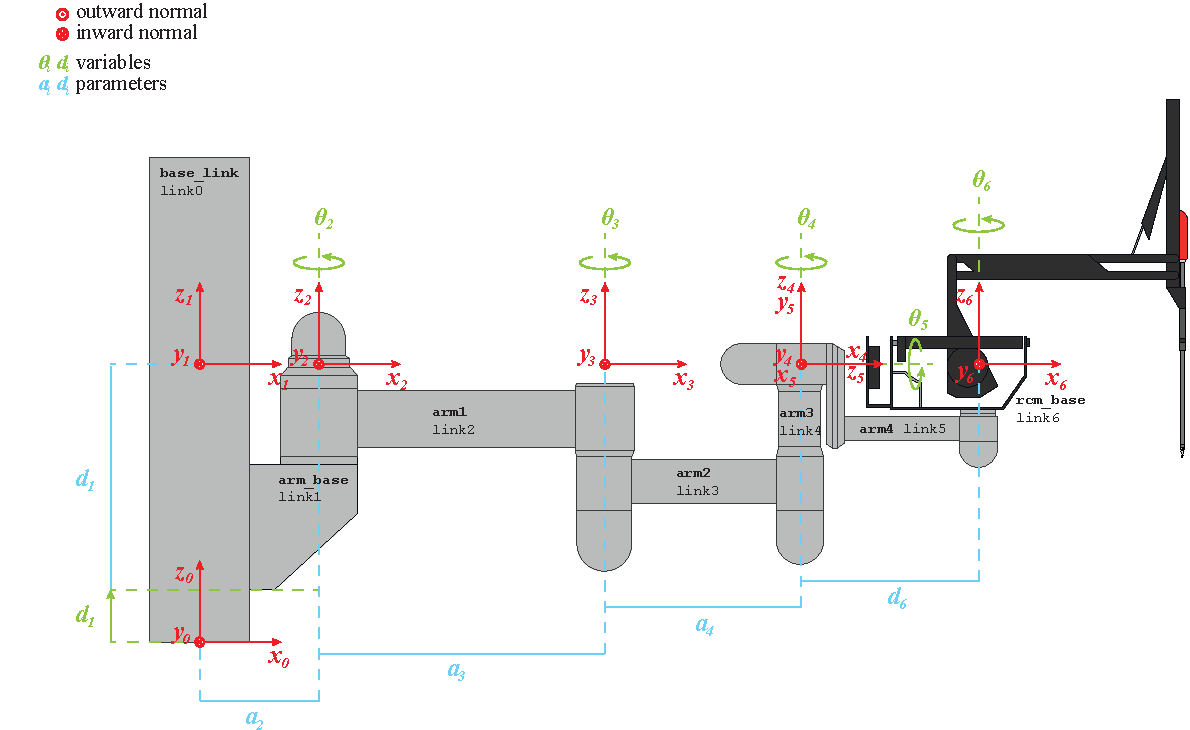
\includegraphics[width=1.1\textwidth]{p4_arm_compromise_frames.pdf}\label{fig:p4_arm_compromise_frames}}%
	\vspace{5mm}\\
	\hspace*{-15mm}
	\subbottom[Coordinate frames for the joints on the robot hand and instrument.]{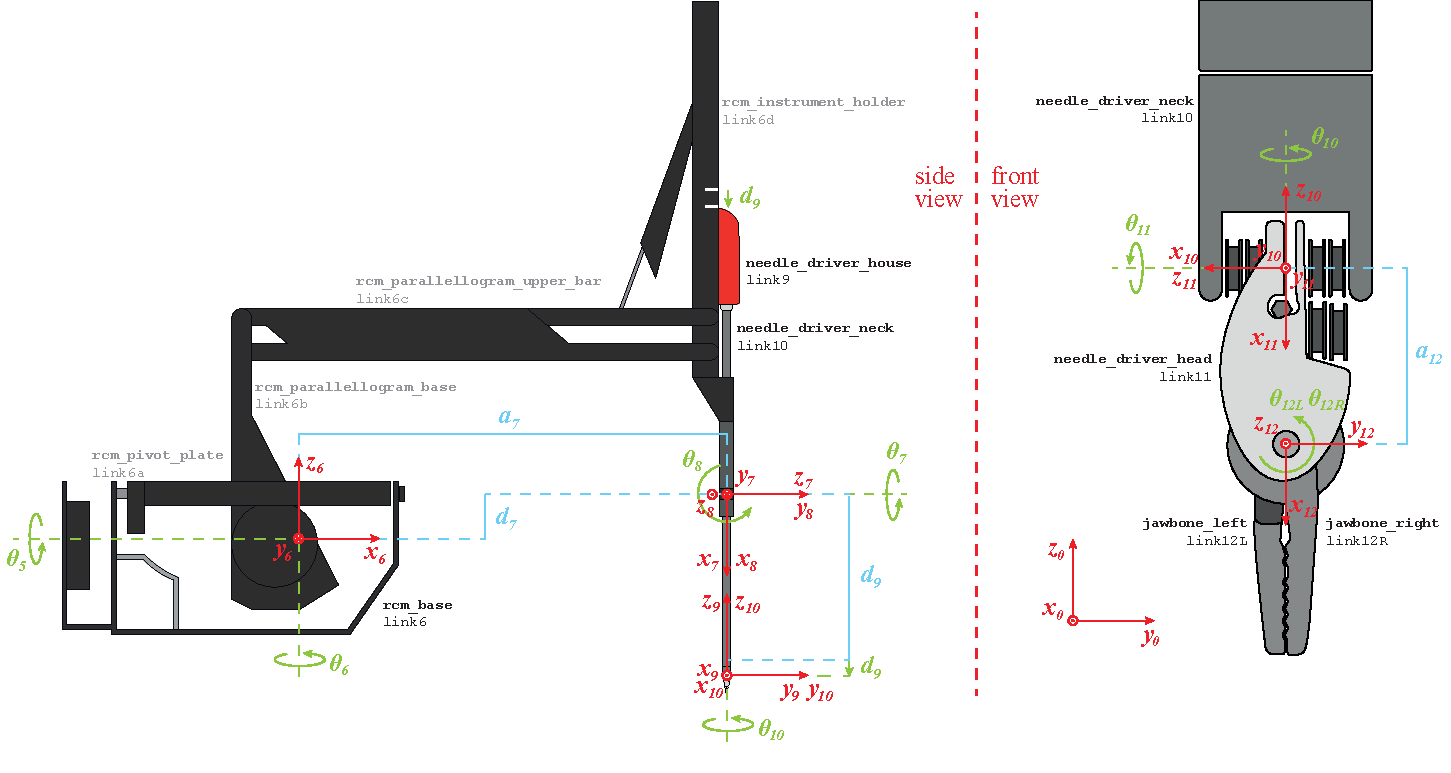
\includegraphics[width=1.15\textwidth]{p4_hand_compromise_frames.pdf}\label{fig:p4_hand_compromise_frames}}%
	\caption{Orientation and position of coordinate frames $\Psi_0$, $\Psi_1$, ..., $\Psi_{12}$ defined according to the compromise between the \gls{dh} convention and the \texttt{xacro} convention.}
	\label{fig:robot_compromise_frames}
\end{figure}

\subsection{Testing Active Joint Kinematics in MATLABb}
As for the previous sets of coordinate frames, the transformations are tested in MATLAB to check the conformity with the two other kinematic chains.
MATLAB script and measurement files can be found in \autoref{app:cd} on the path \texttt{matlab\_scripts/kinematic\_models/robot\_kinematics.m}.

\begin{lstlisting}[language=matlab]
%% Coordinate frames defined as a compromise between DH and the xacro syntax, excluding passive joints
% parameters: distances [m], and rotations [rad]
a = [0 0.198 0.582 0.435 0 0 0.482 0 0.097 0 0 0.009 0.009];
d = [0.998 0 0 0 0 0.412 0.047 0 0 0 0 0 0];
roll = [0 0 0 0 0 0 0 pi/2 0 0 0 -pi/2 -pi/2];
pitch = [0 0 0 0 pi/2 -pi/2 pi/2 0 -pi/2 0 pi/2 0 0];

% Variables (signs are included as long as state comes from old frame convention)
d_free = [d1 0 0 0 0 0 0 0 -d11 0 0 0 0];
theta_free = [0 -th2 -th3 -th4 -th5 th6 th7 th8 0 th12 -th13 th14L -th14R];

% Transformation matrices (forward kinematics)
for i = 1:length(a)
	fixed = [rot(2,pitch(i))*rot(1,roll(i)) [a(i) 0 d(i)]'; zeros(1,3) 1];
	free = [rot(3,theta_free(i)) [0 0 d_free(i)]'; zeros(1,3) 1];
	Trans(:,:,i) = fixed*free;
end
\end{lstlisting}

The new frame transformations result in a set of calculated distances corresponding relatively well to the measured distances, as seen in \autoref{tab:compromise_distances}.

\begin{table}[htbp]
	\centering
\begin{tabular}{l | r r r r}\hline
state as in & table \ref{tab:state0} & table \ref{tab:state5} & table \ref{tab:state6} & table \ref{tab:state7}\\\hline
calculated distance & 2.31\,m & 2.38\,m & 1.85\,m & 2.17\,m\\
measured distance & 2.29\,m & 2.41\,m & 1.89\,m & 2.07\,m\\
\end{tabular}
\caption{Calculated and measured distances between origin of the inertial and the tool tip frames, when using the the active joint kinematics for the calculations.}
\label{tab:compromise_distances}
\end{table}


\textcolor{white}{\gls{rpy}}


\chapter{Dynamic Model of a Beating Heart}\label{app:dynamic_model_heart}
The motion of a point on the surface of the heart can be described as a quasi-periodic rigid 3D motion, which is a combination of the two periodic motions of the diaphragm and the heart \citep{bib:heart_berkeley}. The two separate movements can be described as the vector field \citep{bib:heart_model}

\begin{equation}
\small
x(t_0) = 
\begin{bmatrix}
\sin(\omega_d t_0)\\
\cos(\omega_d t_0)\\
\sin(2 \omega_d t_0)\\
\cos(2 \omega_d t_0)\\
\sin(\tfrac{3}{2}\sin(\omega_d t_0))\\
\cos(\tfrac{3}{2} \sin(\omega_d t_0))\\
\sin(-\tfrac{3}{2} \sin(\omega_d t_0))\\
\cos(-\tfrac{3}{2} \sin(\omega_d t_0))\\
\sin(\omega_h t_0)\\
\cos(\omega_h t_0)\\
\sin(2 \omega_h t_0)\\
\cos(2 \omega_h t_0)\\
\sin(\tfrac{9}{4} \cos(\omega_h t_0))\\
\cos(\tfrac{9}{4} \cos(\omega_h t_0))\\
\sin(\tfrac{6}{8} \cos(2 \omega_h t_0)-\tfrac{9}{8})\\
\cos(\tfrac{6}{8} \cos(2 \omega_h t_0)-\tfrac{9}{8})
\end{bmatrix},
\qquad\qquad
\dot{x}(t) =
\begin{bmatrix}
 \omega_d x_2\\
- \omega_d x_1\\
2  \omega_d x_4\\
-2  \omega_d x_3\\
\tfrac{3}{2}  \omega_d x_2 x_6\\
-\tfrac{3}{2}  \omega_d x_2 x_5\\
-\tfrac{3}{2}  \omega_d x_2 x_8\\
\tfrac{3}{2}  \omega_d x_2 x_7\\
 \omega_h x_10\\
- \omega_h x_9\\
2 \omega_h x_{12}\\
-2 \omega_h x_{11}\\
-\tfrac{9}{4} \omega_h x_9 x_{14}\\
\tfrac{9}{4} \omega_h x_9 x_{13}\\
-\tfrac{6}{8} \omega_h x_{11} x_{16}\\
\tfrac{6}{8} \omega_h x_{11} x_{15}
\end{bmatrix}
+
\begin{bmatrix}
x_2&0\\
-x_1&  0\\
2 x_4& 0\\
-2 x_3&0\\
\tfrac{3}{2} x_2 x_6 & 0\\
-\tfrac{3}{2} x_2 x_5 & 0\\
-\tfrac{3}{2} x_2 x_8 & 0\\
\tfrac{3}{2} x_2 x_7  & 0\\
0& x_{10}\\
0& -x_9\\
0& 2 x_{12}\\
0& -2 x_{11}\\
0& -\tfrac{9}{4} x_9 x_{14}\\
0& \tfrac{9}{4} x_9 x_{13}\\
0& -\tfrac{6}{8} x_{11} x_{16}\\
0& \tfrac{6}{8} x_{11} x_{15}\\
\end{bmatrix}
\cdot d
\end{equation}
\vspace{-3mm}
\begin{tabular}{rll}
where & &\\
$t_0$ & is the start time ($t_0=0$) & [s]\\
$\omega_d$ & is the frequency of the diaphragm movement, read off ECG ($\omega_d=\tfrac{2\pi}{4}$) & [rad/s]\\
$\omega_h$ & is the frequency of the heart movement, read off mechanical ventilator ($\omega_h=\tfrac{2\pi}{1.1}$) & [rad/s]\\
$x_i$ & is the $i$th entry of the state vector $x$ & [$\cdot$]\\
$d$ & is a disturbance vector ($d_1=d_\text{diaphragm}\equiv [-0.4, 0.4]$ and $d_2=d_\text{heart}\equiv [-0.11,0.11]$) & [rad/s]
\end{tabular}
\vspace*{3mm}

The two transformation matrices describing the movement of the diaphragm frame relative to the inertial frame, and the heart frame relative to the diaphragm frame can be composed from the state at time $t$ as \citep{bib:heart_model}
\begin{equation}
^0_dH(t) = 
\begin{bmatrix}
x_6 & x_5 x_8 & x_5 x_7 & 0\\
-x_5 & x_6 x_8 & x_6 x_7 & \tfrac{7}{6} x_4 - \tfrac{7}{6} \\
0 & -x_7 & x_8 & \tfrac{5}{3}x_1\\
0 & 0 & 0 & 1
\end{bmatrix}
\quad\quad
^d_hH(t) = 
\begin{bmatrix}
x_{14} x_{16} & x_{13} & -x_{14} x_{15} & \tfrac{14}{15} x_{10}-2\\
-x_{13}  x_{16} & x_{14} & x_{13} x_{15} & -\tfrac{10}{9} x_9 - \tfrac{10}{9}\\
x_{15} & 0 & x_{16} & 0\\
0 & 0 & 0 & 1
\end{bmatrix}
\end{equation}

The desired position of the robot manipulator can be formulated as the desired transformation (rotation and distance) from the heart (surface point) frame.


%\section{End-effector Set-Point Generator Based on the Beating Heart Model}
%"The estimated components are then combined to predict future motion of the heart surface. This information, in turn, is used in the design of an explicit controller that stabilizes the relative motion of a surgical tool to a desired distance and orientation with respect to the heart surface."
%
%"We then present a control law that uses the predicted motion to asymptotically stabilize the motion of the surgical tool to a desired distance and orientation with respect to the heart surface."
%
%"To simplify the analysis and allow real-time prediction, we do not take the cause of the motion into consideration, and only consider the kinematics of a local area of interest on the heart surface."
%
%"Fortunately, in this application, we have a reasonably good estimate of the phase and frequency of the two motion components: the respiratory phase and frequency can be obtained from the mechanical ventilator, and the cardiac phase and frequency are detected by an ECG monitor."
%
%"choosing a convenient initial position and orientation for $\Psi_d$, e.g. such that $p^d_h(0)=0$ and $R^0_d(0) = I$
%
%Relative configuration between heart and robot tool $H^h_r$ (with $R^h_r =[r_x, r_y, r_z]$) and error function $J(H^h_r)$
%\begin{equation}
%J(H^h_r) = \underbrace{\tfrac{1}{2}k_p (p^h_r-\Delta r_z)^T(p^h_r-\Delta r_z)}_\text{translational error} + \underbrace{k_x (1-e_x^T r_x) + k_y (1-e_y^T r_y) + k_z (1-e_z^T r_z)}_\text{rotational error}
%\end{equation}
%\begin{tabular}{rl}
%	where &\\
%	$\Delta$ & is the desired relative distance between the tool and the heart\\
%	$E=[e_x,e_y,e_z]$ & is a rotation matrix describing the desired orientation of the tool frame\\
%	$k_p,k_x,k_y,k_z$ & are constant positive parameters\\
%\end{tabular}\\
%
%Then $J$ is equal to zero (has its minimum) only when $p^h_r=\Delta r_z$ (the origin of $\Psi_r$ given in h coordinates is $\Delta$ away from the origin of $\Psi_h$ along the surface normal) and $R^h_r=E$ (frame h and r axes are aligned).
%\begin{align}
%	\dot{J} &= 
%	\begin{bmatrix}
%		k_x \hat{e}_x r_x + k_y \hat{e}_y r_y + k_z \hat{e}_z r_z\\
%		k_p(p^h_r - \Delta r_z)
%	\end{bmatrix}^T
%	\begin{bmatrix}
%		\omega^{h,h}_r \\
%		r^{h,h}_r
%	\end{bmatrix}
%	= (dJ)^T T^{h,h}_r\\
%	\dot{H}^h_r &= 
%	\begin{bmatrix}
%		\hat{\omega}^{h,h}_r r_x & \hat{\omega}^{h,h}_r r_y & \hat{\omega}^{h,h}_r r_z & \hat{\omega}^{h,h}_r p^h_r + v^{h,h}_r\\
%		0 & 0 & 0 & 0
%	\end{bmatrix}\\
%	(\dot{dJ}) &=
%	\begin{bmatrix}
%		-k_x \hat{e}_x \hat{r}_x  - k_y \hat{e}_y \hat{r}_y - k_z \hat{e}_z \hat{r}_z & 0\\
%		-k_p(\hat{p}^h_r - \Delta \hat{r}_z) & k_p I
%	\end{bmatrix}
%	T^{h,h}_r
%\end{align}
%
%The relative velocity of two frames, meaning both the linear and angular velocity, can be concisely expressed as a 4x4 matrix (a twist) $T^{c,a}_b$, that describes the relative velocity of frame b with respect to b expressed in frame c
%\begin{equation}
%T^{c,a}_b = H^c_a \dot{H}^a_b H^b_c
%\end{equation}
%
%"We do not consider specific robot dynamics at this point and only specify the desired inertial acceleration $\dot{T}^{0,0}_r$ of the robot end effector frame $\Psi_r$. Proposed desired acceleration"
%\begin{equation}
%\left(\dot{T}^{0,0}_r\right)_\text{des} = \dot{T}^{0,0}_h - \text{Ad}_{H^0_h} K_1 (\dot{dJ}) + \text{ad}_{T^{0,0}_h} T^{0,h}_r - \text{Ad}_{H^0_h} K_2 (T^{h,h}_r + K_1 dJ)
%\end{equation}
%\begin{tabular}{rl}
%	where & \\
%	$K1, K_2$ & are symmetric and positive definite matrices\\
%	$H^0_h$ & is the estimated configuration of the frame $\Psi_h$ at the area of interest on the heart surface\\
%	$T^{0,0}_h$ & is the estimated velocity of the frame $\Psi_h$ at the area of interest on the heart surface\\
%	$\dot{T}^{0,0}_h$ & is the estimated acceleration of the frame $\Psi_h$ at the area of interest on the heart surface\\
%\end{tabular}\\
%
%This controller drives $T^{h,h}_r$ to $-K_1dJ$ by the gain $K_2$, along the steepest descend of $J$. Asymptotic stability at $J=0$, with Lyapunov function
%\begin{equation}
%V=\kappa_1 J + \tfrac{1}{2} (T^{h,h}_r + K_1dJ)^T K_2^{-1}(T^{h,h}_r + K_1dJ)
%\end{equation}
%\begin{tabular}{rl}
%	where & \\
%	$\kappa_1$ & is a positive constant strictly less than 4 times the smallest singular value of $K_1$, $0<\kappa_1 <4\sigma_\text{min}(K_1)$
%\end{tabular}
%
%Assuming the robot achieves perfect tracking of $\left(\dot{T}^{0,0}_r\right)_\text{des}$, the time derivative of $V$ along the system trajectories is
%\begin{equation}
%\dot{V} = -\left(T^{h,h}_r + (K_1 - \tfrac{\kappa_1}{2}I)dJ\right)^T \left(T^{h,h}_r + (K_1 - \tfrac{\kappa_1}{2}I)dJ\right) - \kappa_1(dJ ^T(K_1 - \tfrac{\kappa_1}{4}I)dJ
%\end{equation}
%\begin{tabular}{rl}
%	where & \\
%	$I$ & is the identity matrix\\
%	$K_1 - \tfrac{\kappa_1}{4}$ & is strictly positive because of the choice of $\kappa_1$\\
%\end{tabular}

\chapter{SOSTOOLS Matlab Toolbox}\label{app:sostools}
As presented in \autoref{chap:putinar} a polynomial barrier certificate can be constructed using \gls{sos} optimization by using the MATLAB toolbox SOSTOOLS. This toolbox is a convex relaxation framework based on sum of squares decompositions of multivariate polynomials and semidefinite programming solvers \citep{bib:prajna_framework} (for acquisition, see \autoref{app:sostools}).
In this chapter barrier certificates are sought with SOSTOOLS by use of Putinar's Positivstellensatz, presented in \autoref{def:putinar}.


\section{SOSTOOLS Syntax}
\vspace{-2mm}
An \gls{sos} program is the environment in which the \gls{sos} requirements in \autoref{def:barrier_sos} are set up, and searching for the barrier certificate corresponds to solving the \gls{sos} program.
This section is a short introduction to the SOSTOOLS formulation of the parameters and variables necessary to set up the requirements for the barrier certificate, based on the SOSTOOLS user guide \citep{bib:sostools_manual}.  
An overview of necessary \gls{sos} functions from the toolbox is given in \autoref{tab:sostools_syntax}.

\begin{table}[H]
\begin{tabularx}{\textwidth}{p{6cm} X}
\rowcolor{HeaderBlue}
\textbf{Syntax} & \textbf{Explanation}\\
\texttt{pvar x1;}\newline
\texttt{prog = sosprogram(x1);} & Initialization of an \gls{sos} program \texttt{prog} in the state variable \texttt{x1}, which is declared as  type \texttt{pvar} (or identically as \texttt{syms}, if the MATLAB symbolic toolbox is available)\\
\rowcolor{textBlue} 
\texttt{Z = monomials(x1,deg);}\newline
\texttt{[prog,q] = sossosvar(prog,Z);} & Parametrize an \gls{sos} polynomial \texttt{q} in the \gls{sos} program \texttt{prog}. The degree of the \gls{sos} polynomial is defined by the monomial vector \texttt{Z} of degree \texttt{deg} (i.e. deg(\texttt{q}) $=$ 2\texttt{deg})\\
\texttt{Z = monomials(x1,deg);}\newline
\texttt{[prog,B] = sospolyvar(prog,Z);} & Parametrize a polynomial \texttt{B} in the \gls{sos} program \texttt{prog}. The degree of the  polynomial is defined by the monomial vector \texttt{Z} of degree \texttt{deg} (i.e. deg(\texttt{B}) $=$ \texttt{deg})\\
\rowcolor{textBlue}
%\texttt{prog = soseq(prog,B-q);} & Declare the equality constraint \texttt{B-q} $=0$ in the \gls{sos} program \texttt{prog}\\
\texttt{prog = sosineq(prog,B-q);} & Declare the inequality constraint \texttt{B-q} $\geq 0$ (or more exact: \texttt{B-q} $\in\Sigma[x_1]$) in the \gls{sos} program \texttt{prog}\\
%\rowcolor{textBlue}
\texttt{prog = sossolve(prog);} & Solve the \gls{sos} program \texttt{prog} i.e. find coefficients for all polynomials conforming with all constraints \\
\rowcolor{textBlue}
\texttt{getB = sosgetsol(prog,B)} & After solving, get the solution (with coefficients) for the polynomial \texttt{B}\\
\texttt{[Q,Z,f] = findsos(getB-getq);} &  Test that the solution found complies with the requirement that the inequality is in fact \gls{sos}
\end{tabularx}
\caption{SOSTOOLS functions necessary to search for a barrier function as given by \autoref{def:barrier_sos}.}
\label{tab:sostools_syntax}
\end{table}

\vspace{-1mm}
An \gls{sos} program is initialized with the command \texttt{sosprogram}, and polynomials and \gls{sos} polynomials can be declared in the program in the variables that are input to the program (see \autoref{tab:sostools_syntax}) with \texttt{sospolyvar} and \texttt{sossosvar}, respectively.
%
%where \texttt{degrees} is the degrees of variables desired in the monomial; \texttt{[2 4]} would in this case give that \verb|Z = [x1^2; x1^4]| while \texttt{degrees = 0:2} would result in \verb|Z = [1; x1; x1^2]|. Declaring an SOS polynomial is done similarly to declaring an SOS variable
%
When the necessary SOS variables and polynomials are defined, the inequalities in \autoref{def:barrier_sos} can be defined with the function \texttt{sosineq}, and when all constraints are set up, the program is (attempted to be) solved by calling \texttt{sossolve}. This will return an overview of the precision of the solution (if any was found) as a residual error norm, number of iterations and time elapsed for solving the problem. To get the solution (coefficients) found for any of the SOS variables or polynomials, call the function \texttt{sosgetsol}.



%If no solution could be found, the degree (and thereby complexity) of some SOS variables or polynomials may be increased through their monomials, which may yield a solution to the SOS problem.



\section{Defining a Polynomial Barrier Certificate in SOSTOOLS}\label{sec:app_sostools_barrier_search}
\vspace{-2mm}

Searching for a polynomial barrier certificate in SOSTOOLS require the definition of all of the variables and polynomials given by \autoref{def:barrier_sos} as follows:
\vspace{-2mm}
\renewcommand{\labelitemii}{$\circ$}
\renewcommand{\labelitemiii}{$\bullet$}
\begin{itemize}
	\itemsep-0.7mm
	\item \textbf{Initialize the Program}\\
	First declare the state space variables $x\in\mathbb{R}^n$ as \texttt{syms} or \texttt{pvar}, and initialize the SOS program with the system states by the function \texttt{sosprogram}.
	\item \textbf{Define the Vector Field}\\
	The open-loop state space system $f_{ol}(x)$ is defined, and a controller is found according to pole placement or another preferred method. Then write the closed-loop system equation $f_{cl}$ in terms of the symbolic state vector.
	\item \textbf{Set up the Constraints for the Polynomial Barrier Certificate}\\
	Declare a monomial vector $Z_B$ in $x$ (or part of $x$) of sufficiently large degree, and parametrize the polynomial $B(x)$ as a function of $Z_B$ with \texttt{sospolyvar}.  
	The problem of finding the coefficients for the barrier certificate is now for each region $\mathcal{X}$, $\mathcal{X}_u$ and $\mathcal{X}_0$ a matter of defining the following:
	\vspace*{-1mm}
	\begin{itemize}
		\item \textbf{Define the Polynomials $g_j(x)$}\\
		Define one or more polynomials $g_j$ that are positive in the region to be defined and negative outside. Each polynomial may be solely a function of the robot tool position (and velocity) for static boundaries, and also a function of the heart position (and velocity) for dynamic boundaries. 
		\item \textbf{Declare the SOS Variables $q_j(x)$}\\
		Declare monomial vectors $Z_{q_j}$ in $x$ of appropriate degree (preferably as small as possible to keep the complexity of the problem as low as possible), and parametrize the SOS polynomials (multipliers) $q_j$ with \texttt{sossosvar}.
		\item \textbf{Set up the Inequality}\\
		Cf. the nonnegativity of an \gls{sos} polynomial ($q_0$), each \texttt{sosineq} can be formulated as given by  \autoref{def:barrier_sos}. For \autoref{cer2_putinar} choose a small positive number $\bar{\epsilon}$. The inequality pertaining to a set may be defined in terms of several $g_j$s; if the set is defined by
		\begin{itemize}
			\item $g_1 \bigcap g_2 \bigcap ... \bigcap g_m$, then write $h - \sum q_jg_j\geq 0$
			\item $g_1 \bigcup g_2 \bigcup ... \bigcup g_m$, then write $h - q_1g_1\geq 0$, $h - q_2g_2\geq 0$ etc.
		\end{itemize} 
		Note that each expression in the inequalities in \autoref{def:barrier_sos} must have even degrees in the leading and trailing terms in order for the expressions to be \gls{sos}.
	\end{itemize}
	\item \textbf{Solve the SOS Program}\\
	With all inequalities defined in the program, SOSTOOLS is now ready to solve for the barrier certificate with \texttt{sossolve}, if any certificate exists for the given system $f_{cl}(x)$. If no solution is found, increasing the degree of the \gls{sos} variables $q_j$ or the polynomial $B(x)$ may yield a solution. Otherwise it can be concluded that safety cannot be guaranteed of the  system under scrutiny. 
\end{itemize}





%\textcolor{red}{Matter of defining degree of B and qs - how to decide?}
%In the following section an example is given on how to search for a barrier certificate with SOSTOOLS.


%\textcolor{red}{Og hvordan bruger I så det. Kør eksemplet videre, så det er klart hvordan (8.2e) oversættes til SOS program. Jeg synes I skal køre eksemplet hele vejen igennem og idregne det i SOSTOOLS. På denne måde overbeviser i læseren og, at I kan oversætte teorien til praktisk implementation - Og dette giver points! }




\chapter{Measurement Logs}\label{app:meas}
\lstdefinestyle{DOS}
{
    backgroundcolor=\color{black},
    basicstyle=\scriptsize\color{green}\ttfamily
}
This appendix contains measurement description of most experiments carried out.
\section{Step Response of Slide Position}
The test setup for this test is fairly simple and includes:
\begin{itemize}
\item The Da Vinci robot
\item A laptop (preferable with 10 GB storage available on the AFS drive)
\end{itemize}
The setup is depicted in \autoref{fig:test:slide:pos}.
\begin{figure}[H]\hspace{-1.4cm}
\includegraphics[scale=0.16]{slide_measurement.pdf}
\caption{Test setup to measure slide position}
\label{fig:test:slide:pos}
\end{figure}
\begin{itemize}
\item Configure the ROS environment as described in \autoref{app:ros}, i.e. make sure all low level controllers are running, that \texttt{roscore}, the \texttt{davinci\_driver} and the \texttt{moveit\_group} interface is running.
\end{itemize}
At this point, three terminals should be running. Now, open two additional terminals and prepare both by typing:
\begin{itemize}
\item \texttt{ssh <user name>surgery-srv.lab.es.aau.dk} 
\item \texttt{cd <path to root of workspace>}
\item \texttt{source devel/setup.bash}.
\end{itemize}
\subsection*{First Terminal}
Type:

\hspace{1cm} \texttt{rosrun davinci\_moveit\_config MoveGroupInterfaceExecute}

This launches the \gls{ui} shown below.
\begin{lstlisting}[style=DOS]
Press 'j' to specify joint angles
Press 'x' to specify cartesian positions (IK)
Press 'd' to run demo mode
Press 't' to run test mode
Press 'i' to run IK test 
\end{lstlisting}
Type \textbf{j} + \textbf{enter} to enter custom joint angle mode. It is by default at its zero position for all joint angles. Type 0.005 for slide position and zero for the remaining angles.
\subsection*{Second Terminal}
By subscribing to the \texttt{joint\_state} topic (\texttt{rostopic echo joint\_states}), all information about the current states can be fetched from the sensors, i.e. the potentiometers that measure all joint angles. An example of this is shown below.
\begin{lstlisting}[style=DOS]
---
header: 
  seq: 4553
  stamp: 
    secs: 1428950592
    nsecs: 666452523
  frame_id: ''
name: ['p4_hand_pitch', 'p4_hand_roll', 'p4_instrument_jaw_left', 'p4_instrument_jaw_right', 'p4_instrument_pitch', 'p4_instrument_roll', 'p4_instrument_slide']
position: [-0.021504180505871773, 0.027300411835312843, 0.0006707065622322261, -0.00013414131535682827, 0.0012072718236595392, -0.0896063968539238, 1.055011398420902e-05]
velocity: [0.0, 0.0, 0.0, 0.0, 0.0, 0.0, 0.0]
effort: [-0.5, -0.5, -0.5, -0.5, -0.5, -0.5, -0.5]
---
\end{lstlisting}

For this test, it is more appropriate to merely publish the slide position, this can be done by:

\hspace{1cm}\texttt{rostopic echo joint\_states/position[6]}

Which gives an output as shown below.

\begin{lstlisting}[style=DOS]
---
8.20564400783e-06
---
8.20564400783e-06
---
8.20564400783e-06
---
\end{lstlisting}
Instead of leaving the output as a terminal output, the information is mapped to a \texttt{.txt} file with a suitable name, e.g:

\hspace{1cm} \texttt{rostopic echo joint\_states/position[6] > taus\_05cm\_1\_speedlimit\_100.txt}

Use the MATLAB script and the recorded measurement data found in \autoref{app:cd} under the path \texttt{matlab\_scripts/slide\_step/plot\_slide\_pos.m}, to plot the recorded slide position along with an estimated first and second order approximation. The step response is seen in \autoref{fig:stepresponseslideapp}.
\begin{figure}[H]
\center
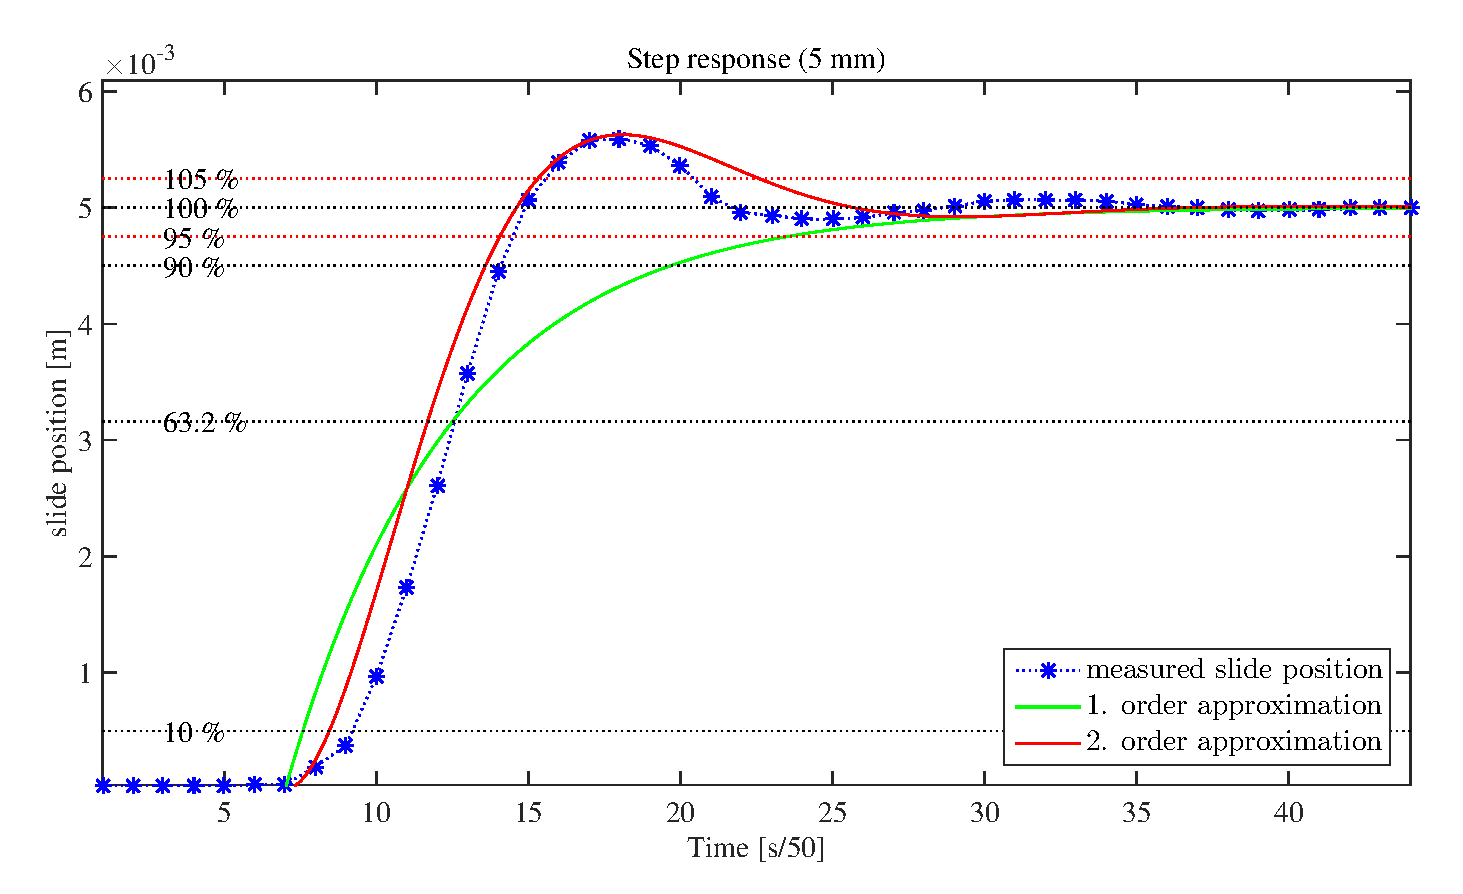
\includegraphics[scale=0.5]{step_slide.eps}
\caption{Step response from 0\,mm to 5\,mm. Plot details and measurements can be found in \autoref{app:cd} as \texttt{matlab\_scripts/slide\_step/plot\_slide\_pos.m}}. 
\label{fig:stepresponseslideapp}
\end{figure}
The approximated second and first order system are found as...????

\chapter{MATLAB Implementation of Control System}
This appendix contains the MATLAB implementation of the controllers developed throughout the project, i.e.:
\begin{itemize}
\item Safety controller for a system with static boundaries for instrument slide in \autoref{sec:app:static}
\item Safety controller for a system with dynamic boundaries to simulate a set-up consisting of a beating hearth and a safe distance between hearth and robot end effector. This is in \autoref{sec:app:dynamic}.
\end{itemize}
\section{Implementation of Instrument Slide Safety Controller with Static Boundaries}\label{sec:app:static}
This section contains the MATLAB implementation of the slide controller developed in \autoref{chap:cbf_1d_static}. No user inputs are required to run the script. The script shown here includes no plotting, but the script found in \autoref{app:cd} under the path \texttt{matlab\_scripts/slide\_controller/slide\_controller.m} includes all plotting details.\\

\begin{lstlisting}[language=matlab]
model = 2; % 1 = first order model, 2 = second order model

%--- parabola coeficients for position constraints ---%
a = 16/9; b = 4/45; c = -2/225; 
%--- elliptic paraboloid  coeficients for position constraints ---%
x10 = 1/40; x20 = 0; a1 = -3/40; b1 = -10; c1 = 1; c2 = -1;

if model == 2
    s = tf('s'); % prepare Laplace operator
    ts = (28-9)*1/50; % 5 percent settling time
    tr = 0.1; % rise time
    wn = 1.8/tr; % calculate natural frequency
    zeta = -1/(wn*ts)*log(0.02); % calculate the damping ratio
    H = wn^2/(s^2 + 2*zeta*wn*s + wn^2); % calculate transfer function
    num = wn^2; % Specify numarator
    den = [1 2*zeta*wn wn^2]; % specify denominator
    A = [0 1; -wn^2 -2*zeta*wn];
    B = [0 wn^2]';
    C = [1 0];
    D = 0;
    sys = ss(A,B,C,D)
    x(1,1) = 0 % initial state position
    x(2,1) = 0; % initial state velocity
    K = acker(sys.a,sys.b,[-14 -15]);
elseif model == 1
    tau = 0.110; % time constant
    a_sys = -1/tau; %
    b_sys = 1/tau; % sine wave frequency
    sys = ss(a_sys,b_sys,1,0);
    x(1,1) = 0; % initial state;
    K = acker(a_sys,b_sys,[1.1*eig(sys.a)]); % control gain   
end

kappa = 1; % design parameter
Nbar = - inv(sys.c*inv(sys.a-sys.b*K)*sys.b); % ensure unity gain
scrsz = get(groot,'ScreenSize'); % get screen information

%--- Find epsilon ---%
x_epsilon = 0.04; % find epsilon from desired soft limit
epsilon = a*x_epsilon^2 + b*x_epsilon + c; % find epsilon
syms x0
softlims = solve(a*x0^2 + b*x0 + c == epsilon); % find soft limits
epsilon = abs(epsilon); % specify ep silon as a positive number

%--- make reference vector ---%
XREF = [0.02 0.09 -0.14 -0.02 0.045 0.01]; % simulation setpoints
xref = XREF(1); % initial reference

f = 100; Ts = 1/f; % sampling frequency
N = 5; % simulation time in seconds
fprintf('Simulation time: %d seconds\n', N)

i = (0:Ts:N); % make simulation resolution realistic
utilde = zeros(round(length(i)),1); % init utilde
Rplot(1) = 1; % init reference plot

for R = 1:length(i)
  %--- set various references ---%
  REFS = 6;
  if R == round(length(i)/REFS)*1
      xref = XREF(2);
      Rplot(2) = R;
  elseif R == round(length(i)/REFS)*2
      xref = XREF(3);
      Rplot(3) = R;
  elseif R == round(length(i)/REFS)*3
      xref = XREF(4);
      Rplot(4) = R;
  elseif R == round(length(i)/REFS)*4
      xref = XREF(5);
      Rplot(5) = R;
  elseif R == round(length(i)/REFS)*5
      xref = XREF(6);
      Rplot(6) = R;
  end
  
  %--- physical constraints for velocity  ---%
  if 1
    if model == 2
      max_vel = 1;
      if x(2,R) > max_vel
          x(2,R) = max_vel;
      elseif x(2,R) < -max_vel
          x(2,R) = -max_vel;
      end
    end
  end
 
  %--- output ---%
  y(:,R) = sys.C*x(:,R);
  
  %--- determine sigma  ---% 
  if model == 1
      if (a*(x(1,R))^2 + b*(x(1,R)) + c) <= -epsilon
          sigma = 0;
      elseif ((a*(x(1,R)).^2 + b*(x(1,R)) + c) > -epsilon) && ...
             ((a*(x(1,R)).^2 + b*(x(1,R)) + c) <  0)
          sigma = -2*((a*(x(1,R)).^2 + b*(x(1,R)) + c)/epsilon).^3 - ...
                   3.*((a*(x(1,R)).^2 + b*(x(1,R)) + c)/epsilon ).^2 + 1;
      else
          sigma = 1;
      end
  elseif model == 2
      cbf = (a.*(x(1,R)).^2 + b.*x(1,R) + c);
      if cbf <= -epsilon
          sigma = 0;
      elseif (cbf > -epsilon) && (cbf < 0)
          if model == 1
              sigma = -2*((a*(x(1,R)).^2 + b*(x(1,R)) + c)/epsilon).^3 - ...
                       3.*((a*(x(1,R)).^2 + b*(x(1,R)) + c)/epsilon ).^2 + 1;
          elseif model == 2
              sigma = -2*((a*(x(1,R)).^2 + b*(x(1,R)) + c)/epsilon).^3 - ...
                       3.*((a*(x(1,R)).^2 + b*(x(1,R)) + c)/epsilon ).^2 + 1;
          end
      else
          sigma = 1;
      end 
  end

  %--- print every thousand iteration to user ---%
  if mod(R,1000) == 1 
      if R ~= 1
          fprintf('iter = %d of %d\n', R-1, length(i)-1);
      else
          fprintf('iter = %d of %d\n', R, length(i)-1);
      end
  end

  %--- find lie derivatives ---%
  if model == 2
      LgB(1,R) = (c1*wn^2*(2*x(2,R) + 2*x20))/b1^2;
      LfB(1,R) = (c1*x(2,R)*(2*x(1,R) + 2*x10))/a1^2 - ...
          (c1*(2*x(2,R) + 2*x20)*(x(1,R)*wn^2 + 2*x(2,R)*zeta*wn))/b1^2; 
  elseif model == 1
      LgB(1,R) = (2*(a)*(x(:,R)) + (b))*(sys.b);
      LfB(1,R) = (2*(a)*(x(:,R)) + (b))*((sys.a)*x(:,R));
  end
  
  %-- Find controller by pole placement --%
  utilde(1,R) = xref*Nbar - K*x(:,R);

  %--- Find safe controller ---%
  threshold = 0.001;
  if abs(LgB(1,R)) >= threshold
      k0(1,R) = -( ( LfB(1,R) + sqrt(LfB(1,R)^2 ...
          + kappa^2*LgB(1,R)*LgB(1,R)' )) /  (LgB(1,R)*LgB(1,R)')  ) *LgB(1,R);
      kplot(1,R) =  k0(1,R);
  else
      k0(1,R) = 0;
      kplot(1,R) = k0(1,R);
  end 
  
  %--- control law ---%
  u0(1,R) = sigma*k0(1,R)+(1-sigma)*utilde(1,R);
  
  %--- physical constraints for control signal  ---%
  slide_lim = 0.1;
  if u0(1,R) > slide_lim
      u0(1,R) = slide_lim;
  elseif u0(1,R) < -slide_lim
      u0(1,R) = -slide_lim;
  end
 
  %--- save the LfclB ---%
  LfclB(1,R) = LfB(1,R) + LgB(1,R).*k0(1,R);
  
  %--- extrapolate with forward euler ---%
  xdot = sys.a*x(:,R) + u0(1,R)*sys.b;
  x(:,R+1) = xdot*Ts + x(:,R);
  sig(1,R) = sigma;
  
end
\end{lstlisting}
\section{Implementation of Instrument Slide Safety Controller with Dynamic Boundaries}\label{sec:app:dynamic}
This section contains MATLAB implementation of the controller developed in \autoref{chap:cbf_1d_dynamic}. All plotting details are omitted in this section, but the controller can also be found in \autoref{app:cd} under the path \texttt{matlab\_scripts/beating\_hearth/beating\_hearth\_controller.m} which includes the plotting section as well.\\

\begin{lstlisting}[language=matlab]
%--- setup systems ---%
k = 9;
Nbar = 10;
tau = 0.110;
wh = 2*pi/1.1;
A = [-1/tau  0   0  0;
      0      0   wh 0;
      0     -wh  0  0;
      0      0   0  0];
B = [(1/tau) 0 0 0]';
K = [-k Nbar 0 Nbar];

%--- initial conditions ---%
x(1,1) = 0.05; % initial state position
x(2,1) = -0.03; % initial hearth position
x(3,1) = 0; % initial hearth velocity
x(4,1) = 0.03; % initial distance

kappa = 1;
scrsz = get(groot,'ScreenSize'); % get screen information

f = 2000; Ts = 1/f; % sampling frequency
N = 5; % simulation time in seconds
fprintf('Simulation time: %d seconds\n', N)

i = (0:Ts:N); % make simulation resolution realistic
utilde = zeros(round(length(i)),1); % init utilde
Rplot(1) = 1; % init reference plot

%--- run controller ---%
epsilon = 0.01; 
for R = 1:length(i)
    
  if mod(R,1000) == 1 
      if R ~= 1
          fprintf('iter = %d of %d\n', R-1, length(i)-1);
      else
          fprintf('iter = %d of %d\n', R, length(i)-1);
      end
  end
  
  %--- give an unsafe distance ---%
  if R > f*2 
      x(4,R) = -0.01;
  end
  
  cbf = x(2,R) - x(1,R);
  %--- determine sigma  ---% 
  if cbf <= -epsilon
      sigma = 0;
  elseif ( (cbf > -epsilon) && (cbf <  0)   )
      sigma = -2*(cbf/epsilon).^3 - 3.*(cbf/epsilon).^2 + 1;
  else
      sigma = 1;
  end
  %sigma = 0;

  %--- find lie derivatives ---%
  LgB(1,R) = -1/tau;
  LfB(1,R) = wh*x(3,R) + x(1,R)/tau;
  
  %-- Find controller by pole placement --%
  utilde(1,R) = K*x(:,R);

  %--- Find safe controller ---%
  threshold = 0.001;
  if abs(LgB(1,R)) >= threshold
      k0(1,R) = -( ( LfB(1,R) + sqrt(LfB(1,R)^2 ...
          + kappa^2*LgB(1,R)*LgB(1,R)' )) /  (LgB(1,R)*LgB(1,R)')  ) *LgB(1,R);
      kplot(1,R) =  k0(1,R);
  else
      k0(1,R) = 0;
      kplot(1,R) = k0(1,R);
  end 

  %--- control law ---%
  u0(1,R) = sigma*k0(1,R)+(1-sigma)*utilde(1,R);
  
  %--- save the LfclB ---%  
  LfclB(1,R) = LfB(1,R) + LgB(1,R).*k0(1,R);
  
  %--- extrapolate with forward euler ---%
  %xdot = A*(x(:,R) + [0 0.2 0.2 0]') + u0(1,R)*B;
  xdot = A*x(:,R) + u0(1,R)*B;
  x(:,R+1) = xdot*Ts + x(:,R);
  
  %--- record sigma ---%
  sig(1,R) = sigma;

  %--- ---% calculate distance between hearth and robot end effector ---%
  Delta(1,R) = x(1,R) - x(2,R);
end
\end{lstlisting}\label{app:slide_implement_1}

\end{appendices}
\end{document}